\documentclass[11pt]{article}
\usepackage[margin=2cm]{geometry}
\usepackage{amsmath,amssymb}
\usepackage{graphicx}
\usepackage{booktabs}
\usepackage{array}
\usepackage{xcolor}
\usepackage[breakable]{tcolorbox}
\usepackage{enumitem}
\usepackage[hidelinks]{hyperref}
\allowdisplaybreaks
\setlength{\parindent}{0pt}
\setlength{\parskip}{4pt}
\definecolor{stepc}{HTML}{1F4E9E}
\definecolor{ansc}{HTML}{0B6E4F}
\newcommand{\solstep}[2]{\par\medskip{\color{stepc}\textbf{Step #1 --- #2}}\par\nopagebreak}
\newtcolorbox{probbox}[1]{colback=white,colframe=black!55,fonttitle=\bfseries,title={#1}}
\newtcolorbox{ansbox}{breakable,colback=ansc!6,colframe=ansc,fonttitle=\bfseries,title={Answer}}
\newtcolorbox{cardbox}[1]{breakable,colback=stepc!4,colframe=stepc,fonttitle=\bfseries,title={#1}}
\graphicspath{{../../../output/lecture5/5E_amplifier_design/}}
\title{Set 5E: MOSFET Amplifier Design}
\author{ECEN 325 --- Lecture 5 (MOS Field-Effect Transistors) practice set}
\date{}
\begin{document}
\maketitle

\textbf{What this set trains.} Designing a MOSFET amplifier from a specification table with the procedure of
Sample Problem 5: the load current sizes the current sink of the output follower, the follower gain tells how much the
common-source drain must swing, the supply budget bounds $V_{R4}$, the gain fixes $V_{ov1} = 2V_{R4}/|A_{v1}|$, and the
input resistance fixes the gate divider. Every design is checked by analysing the finished circuit (DC point, exact
gain, swing limits, distortion). Problems 1--6 are easy, 7--12 medium, 13--18 hard. Try each problem before looking
at its solution.


\begin{cardbox}{The Lecture-5 pipeline (use it for every problem in this lecture)}
\textbf{Tools --- this is all the theory you need (plus the Lecture-1--4 tools):}
\begin{enumerate}[label=\textbf{T\arabic*},leftmargin=2.2em,itemsep=1pt]
\item \emph{Square law} ($I_G = 0$ always). NMOS: $V_{ov} = V_{GS} - V_{tn}$; PMOS: $V_{ov} = V_{SG} - |V_{tp}|$.
      Cutoff if $V_{ov}\le 0$; active (saturation) if $|V_{DS}| \ge V_{ov}$:
      $I_D = \frac{k'}{2}\frac{W}{L}V_{ov}^2$; otherwise triode.
      A diode-connected transistor (gate tied to drain) is always active.
\item \emph{One quadratic per transistor:} with the gate voltage known, KVL gate $\to$ source $\to$ resistor $\to$
      known node gives $V_{known} = V_{GS} + R\,I_D$ with $I_D = \frac{k}{2}(V_{GS}-V_t)^2$. Of the two roots keep
      the one with $V_{GS} > V_t$.
\item \emph{Current mirror:} transistors with the same gate node and the same source node have the same $V_{GS}$,
      so their currents scale with $W/L$: $\frac{I_{D2}}{I_{D1}} = \frac{(W/L)_2}{(W/L)_1}$.
\item \emph{Small signal} ($r_o = \infty$): $g_m = k'\frac{W}{L}V_{ov} = \sqrt{2k'\frac{W}{L}I_D} = \frac{2I_D}{V_{ov}}$.
      Node impedances: $Z_{gate} = \infty$, $Z_{drain} = \infty$, $Z_{source} = \frac{1}{g_m}$. Gains: CS
      $\frac{v_d}{v_g} = -\frac{Z_D}{1/g_m + Z_S}$, CD $\frac{v_s}{v_g} = \frac{Z_S}{1/g_m + Z_S}$, CG
      $\frac{v_d}{v_s} = \frac{Z_D}{1/g_m}$ ($Z_D$, $Z_S$: everything else hanging on that node). For AC, DC supplies
      are ground and ``$\infty$'' capacitors are shorts.
\item \emph{Thevenin:} a linear network seen from two terminals is a source $V_{th}$ (its open-circuit voltage) in
      series with $R_{th}$ (its resistance with all sources set to zero). Branches $(V_k, R_k)$ in parallel combine to
      $V_{th} = \frac{\sum V_k/R_k}{\sum 1/R_k}$, $R_{th} = R_1\|R_2\|\dots$; a series resistor adds to $R_{th}$.
\end{enumerate}
\textbf{Steps:}
\begin{enumerate}[leftmargin=2.2em,itemsep=1pt]
\item \emph{DC:} assume every transistor active; gate voltages from dividers ($I_G=0$); one quadratic (or a mirror
      ratio) per transistor; then node voltages by KCL; \emph{verify} $V_{ov} > 0$ and $|V_{DS}| \ge V_{ov}$.
\item \emph{AC:} $g_m$ of every transistor; node impedances; multiply the node-to-node gains along the signal path;
      then standard form, Bode plot and output as in Lecture 1.
\item \emph{Design:} run the same relations backwards with the stated design rules, then check by analysis.
\end{enumerate}
\end{cardbox}

\section*{Problems}
\subsection*{Easy problems}
\begin{probbox}{Problem 5E.1 \hfill Easy}
Design the amplifier below (find all resistor values) for the specifications in the table. Assume $k'_p\frac{W}{L} = 1\,\mathrm{m}\mathrm{A/V^2}$, $V_{tp} = -1$\,V, $r_o = \infty$; capacitors marked $\infty$ are shorts at the signal frequency. Design choices: $V_{R4} = 5$\,V.

\smallskip\noindent\begin{minipage}{0.6\linewidth}\centering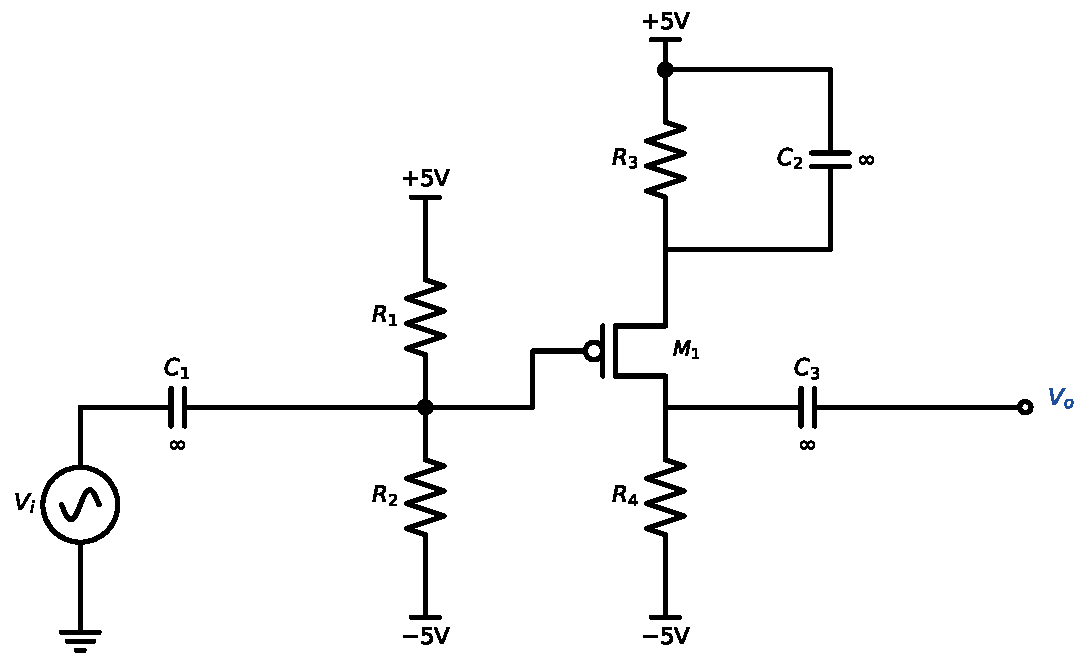
\includegraphics[width=\linewidth,height=6cm,keepaspectratio]{p01_circuit}\end{minipage}\hfill\begin{minipage}{0.38\linewidth}\begin{center}\small\renewcommand{\arraystretch}{1.35}
\begin{tabular}{ll}
\toprule
specification & value \\
\midrule
Dual supply voltage & $+5$\,V / $-5$\,V \\
0-to-peak output swing $\hat V_o$ & $\ge 2$\,V \\
Voltage gain $|A_v|$ & $20$ \\
Input resistance $R_i$ & $\ge 100\,\mathrm{k}\Omega$ \\
THD at $\hat V_o = 2$\,V & $\le 6\,\%$ \\
DC voltage drop on $R_3$ & $\ge 0.5$\,V \\
\bottomrule
\end{tabular}\end{center}
\end{minipage}
\end{probbox}

\begin{probbox}{Problem 5E.2 \hfill Easy}
Design the amplifier below (find all resistor values) for the specifications in the table. Assume $k'_n\frac{W}{L} = 1\,\mathrm{m}\mathrm{A/V^2}$, $V_{tn} = 1$\,V, $r_o = \infty$; capacitors marked $\infty$ are shorts at the signal frequency. Design choices: $V_{R4} = 5$\,V.

\smallskip\noindent\begin{minipage}{0.6\linewidth}\centering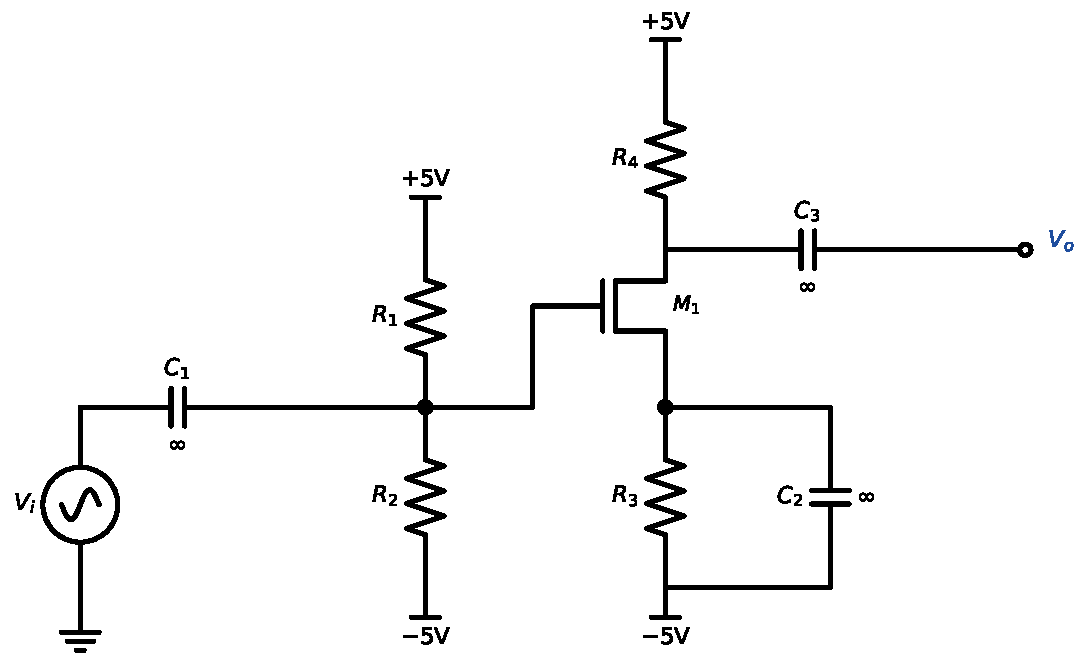
\includegraphics[width=\linewidth,height=6cm,keepaspectratio]{p02_circuit}\end{minipage}\hfill\begin{minipage}{0.38\linewidth}\begin{center}\small\renewcommand{\arraystretch}{1.35}
\begin{tabular}{ll}
\toprule
specification & value \\
\midrule
Dual supply voltage & $+5$\,V / $-5$\,V \\
0-to-peak output swing $\hat V_o$ & $\ge 1.5$\,V \\
Voltage gain $|A_v|$ & $25$ \\
Input resistance $R_i$ & $\ge 200\,\mathrm{k}\Omega$ \\
THD at $\hat V_o = 1.5$\,V & $\le 5\,\%$ \\
DC voltage drop on $R_3$ & $\ge 1$\,V \\
\bottomrule
\end{tabular}\end{center}
\end{minipage}
\end{probbox}

\begin{probbox}{Problem 5E.3 \hfill Easy}
Design the amplifier below (find all resistor values) for the specifications in the table. Assume $k'_p\frac{W}{L} = 2\,\mathrm{m}\mathrm{A/V^2}$, $V_{tp} = -0.8$\,V, $r_o = \infty$; capacitors marked $\infty$ are shorts at the signal frequency. Design choices: $V_{R4} = 6$\,V.

\smallskip\noindent\begin{minipage}{0.6\linewidth}\centering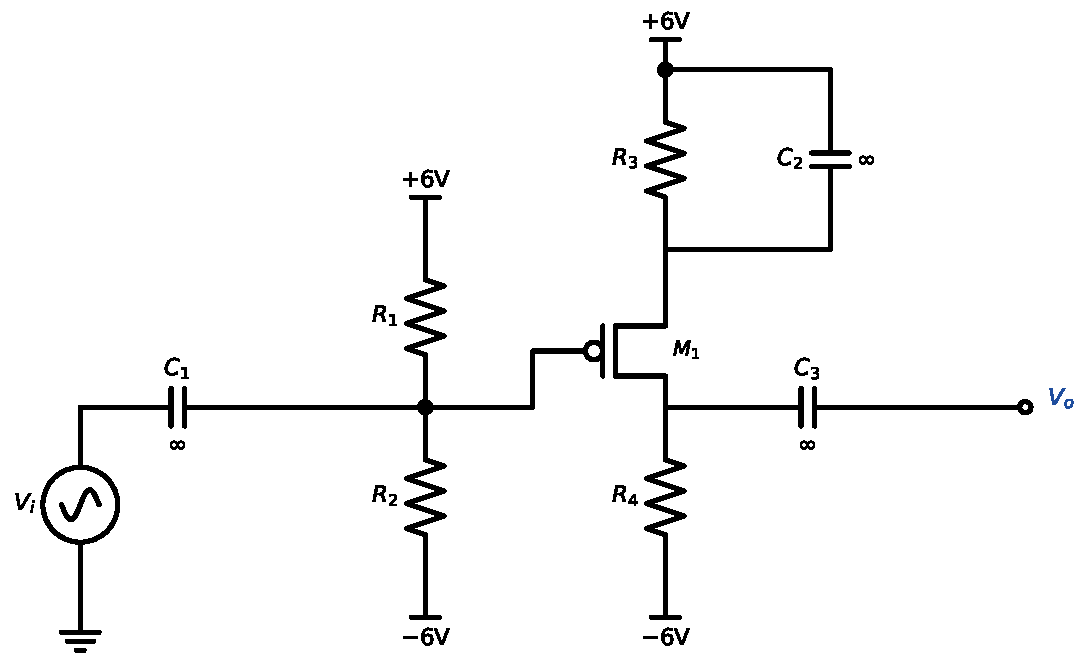
\includegraphics[width=\linewidth,height=6cm,keepaspectratio]{p03_circuit}\end{minipage}\hfill\begin{minipage}{0.38\linewidth}\begin{center}\small\renewcommand{\arraystretch}{1.35}
\begin{tabular}{ll}
\toprule
specification & value \\
\midrule
Dual supply voltage & $+6$\,V / $-6$\,V \\
0-to-peak output swing $\hat V_o$ & $\ge 2$\,V \\
Voltage gain $|A_v|$ & $15$ \\
Input resistance $R_i$ & $\ge 100\,\mathrm{k}\Omega$ \\
THD at $\hat V_o = 2$\,V & $\le 5\,\%$ \\
DC voltage drop on $R_3$ & $\ge 1$\,V \\
\bottomrule
\end{tabular}\end{center}
\end{minipage}
\end{probbox}

\begin{probbox}{Problem 5E.4 \hfill Easy}
Design the amplifier below (find all resistor values) for the specifications in the table. Assume $k'_n\frac{W}{L} = 500\,\mu \mathrm{A/V^2}$, $V_{tn} = 0.7$\,V, $r_o = \infty$; capacitors marked $\infty$ are shorts at the signal frequency. Design choices: $V_{R4} = 3$\,V.

\smallskip\noindent\begin{minipage}{0.6\linewidth}\centering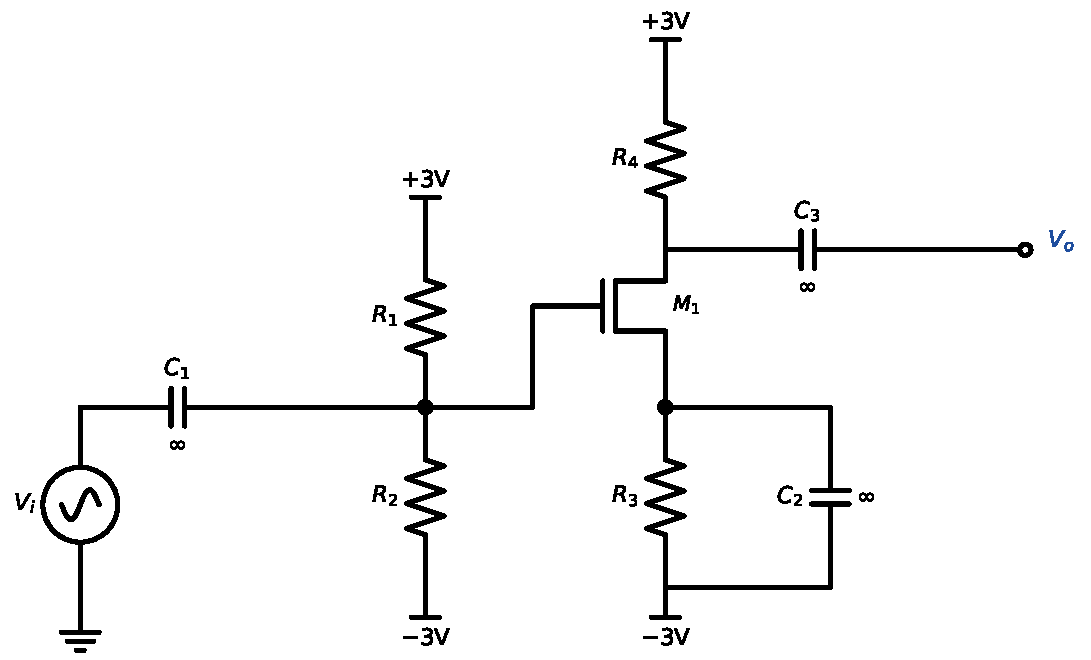
\includegraphics[width=\linewidth,height=6cm,keepaspectratio]{p04_circuit}\end{minipage}\hfill\begin{minipage}{0.38\linewidth}\begin{center}\small\renewcommand{\arraystretch}{1.35}
\begin{tabular}{ll}
\toprule
specification & value \\
\midrule
Dual supply voltage & $+3$\,V / $-3$\,V \\
0-to-peak output swing $\hat V_o$ & $\ge 1$\,V \\
Voltage gain $|A_v|$ & $10$ \\
Input resistance $R_i$ & $\ge 50\,\mathrm{k}\Omega$ \\
THD at $\hat V_o = 1$\,V & $\le 5\,\%$ \\
DC voltage drop on $R_3$ & $\ge 0.5$\,V \\
\bottomrule
\end{tabular}\end{center}
\end{minipage}
\end{probbox}

\begin{probbox}{Problem 5E.5 \hfill Easy}
Design the amplifier below (find all resistor values) for the specifications in the table. Assume $k'_p\frac{W}{L} = 1\,\mathrm{m}\mathrm{A/V^2}$, $V_{tp} = -1$\,V, $r_o = \infty$; capacitors marked $\infty$ are shorts at the signal frequency. Design choices: $V_{R4} = 6$\,V.

\smallskip\noindent\begin{minipage}{0.6\linewidth}\centering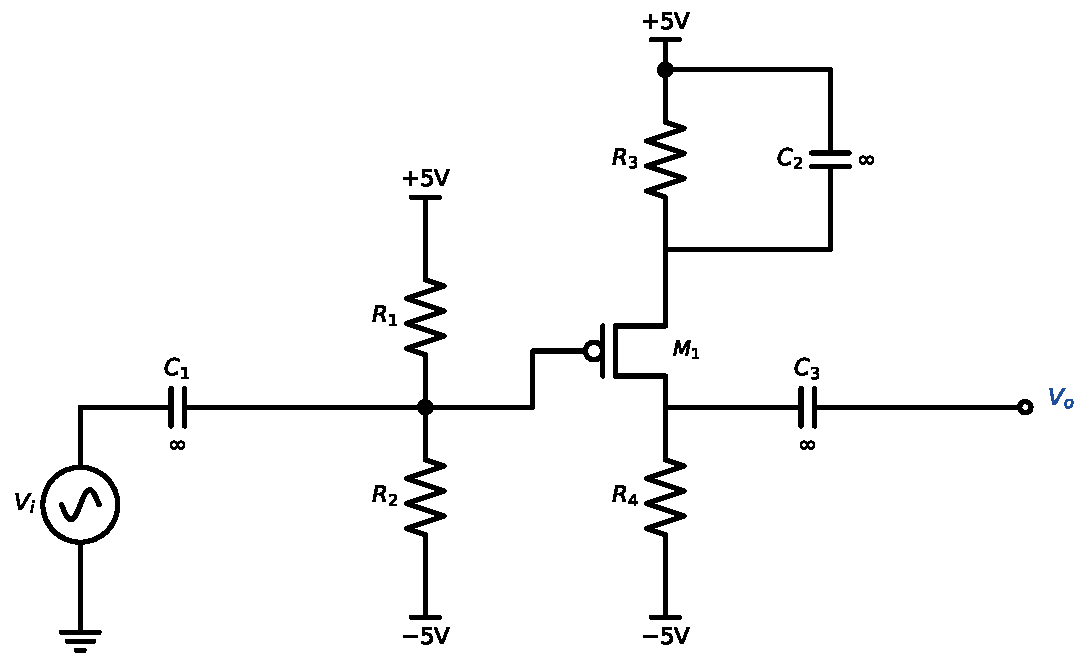
\includegraphics[width=\linewidth,height=6cm,keepaspectratio]{p05_circuit}\end{minipage}\hfill\begin{minipage}{0.38\linewidth}\begin{center}\small\renewcommand{\arraystretch}{1.35}
\begin{tabular}{ll}
\toprule
specification & value \\
\midrule
Dual supply voltage & $+5$\,V / $-5$\,V \\
0-to-peak output swing $\hat V_o$ & $\ge 1$\,V \\
Voltage gain $|A_v|$ & $40$ \\
Input resistance $R_i$ & $\ge 1\,\mathrm{M}\Omega$ \\
THD at $\hat V_o = 1$\,V & $\le 3\,\%$ \\
DC voltage drop on $R_3$ & $\ge 0.5$\,V \\
\bottomrule
\end{tabular}\end{center}
\end{minipage}
\end{probbox}

\begin{probbox}{Problem 5E.6 \hfill Easy}
Design the amplifier below (find all resistor values) for the specifications in the table. Assume $k'_n\frac{W}{L} = 1\,\mathrm{m}\mathrm{A/V^2}$, $V_{tn} = 1$\,V, $r_o = \infty$; capacitors marked $\infty$ are shorts at the signal frequency. Design choices: $V_{R4} = 9$\,V.

\smallskip\noindent\begin{minipage}{0.6\linewidth}\centering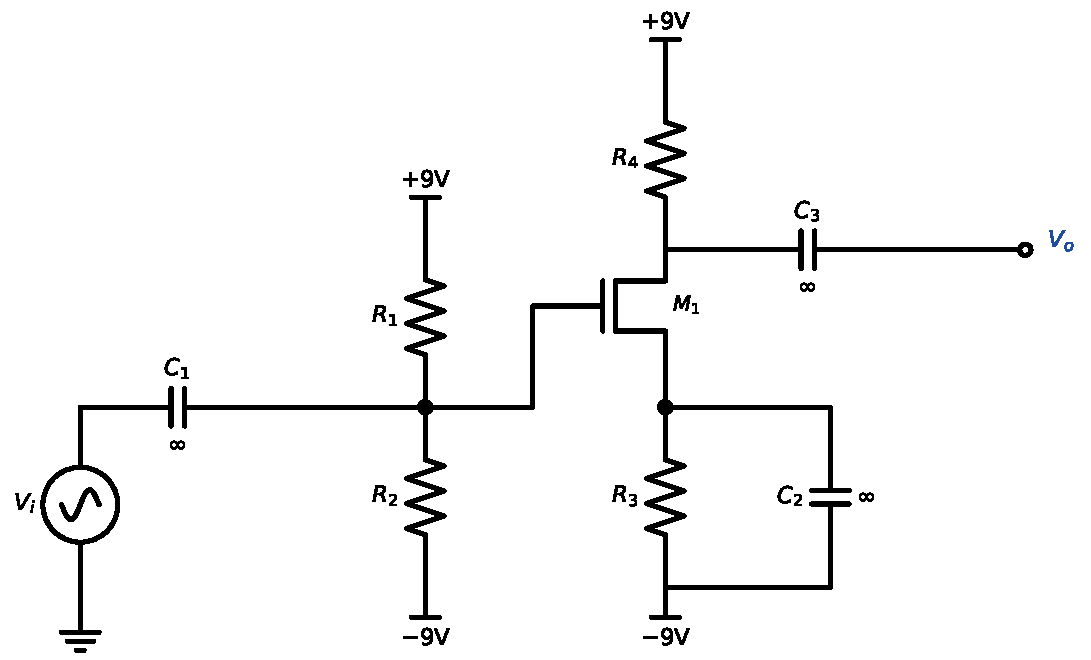
\includegraphics[width=\linewidth,height=6cm,keepaspectratio]{p06_circuit}\end{minipage}\hfill\begin{minipage}{0.38\linewidth}\begin{center}\small\renewcommand{\arraystretch}{1.35}
\begin{tabular}{ll}
\toprule
specification & value \\
\midrule
Dual supply voltage & $+9$\,V / $-9$\,V \\
0-to-peak output swing $\hat V_o$ & $\ge 3$\,V \\
Voltage gain $|A_v|$ & $30$ \\
Input resistance $R_i$ & $\ge 500\,\mathrm{k}\Omega$ \\
THD at $\hat V_o = 3$\,V & $\le 5\,\%$ \\
DC voltage drop on $R_3$ & $\ge 1$\,V \\
\bottomrule
\end{tabular}\end{center}
\end{minipage}
\end{probbox}

\subsection*{Medium problems}
\begin{probbox}{Problem 5E.7 \hfill Medium}
Design the amplifier below (find all resistor values) for the specifications in the table. Assume $k'_n\frac{W}{L} = 50\,\mathrm{m}\mathrm{A/V^2}$, $V_{tn} = 2$\,V, $k'_p\frac{W}{L} = 1\,\mathrm{m}\mathrm{A/V^2}$, $V_{tp} = -1$\,V; $M_2$, $M_3$ (and $M_4$) have the same $k$, $r_o = \infty$; capacitors marked $\infty$ are shorts at the signal frequency. Design choices: $I_{D3} = 10\,\mathrm{m}\mathrm{A}$; $V_{R3}$ at its minimum and $V_{R4}$ at the next multiple of 0.5\,V above its lower bound.\begin{center}\small\renewcommand{\arraystretch}{1.35}
\begin{tabular}{ll}
\toprule
specification & value \\
\midrule
Dual supply voltage & $+5$\,V / $-5$\,V \\
Load resistance $R_L$ & $200\,\Omega$ \\
0-to-peak output swing $\hat V_o$ & $\ge 1$\,V \\
Voltage gain $|A_v|$ & $20$ \\
Input resistance $R_i$ & $\ge 100\,\mathrm{k}\Omega$ \\
THD at $\hat V_o = 1$\,V & $\le 10\,\%$ \\
DC voltage drop on $R_3$ & $\ge 0.5$\,V \\
\bottomrule
\end{tabular}\end{center}

\begin{center}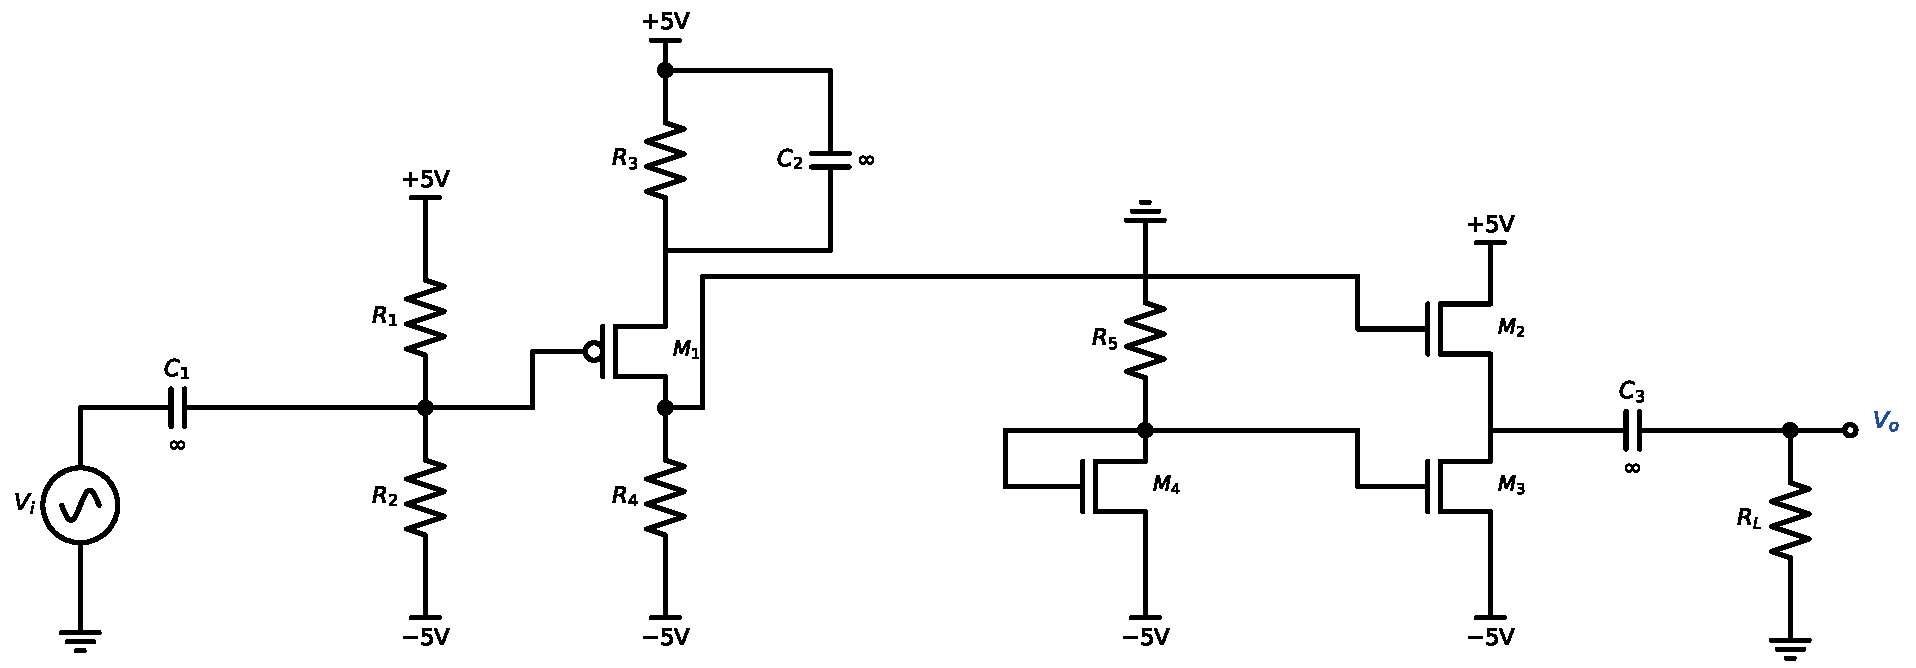
\includegraphics[width=\linewidth,height=6cm,keepaspectratio]{p07_circuit}\end{center}
\end{probbox}

\begin{probbox}{Problem 5E.8 \hfill Medium}
Design the amplifier below (find all resistor values) for the specifications in the table. Assume $k'_n\frac{W}{L} = 50\,\mathrm{m}\mathrm{A/V^2}$, $V_{tn} = 2$\,V, $k'_p\frac{W}{L} = 1\,\mathrm{m}\mathrm{A/V^2}$, $V_{tp} = -1$\,V; $M_2$, $M_3$ (and $M_4$) have the same $k$, $r_o = \infty$; capacitors marked $\infty$ are shorts at the signal frequency. Design choices: $I_{D3} = 5\,\mathrm{m}\mathrm{A}$; $V_{R3}$ at its minimum and $V_{R4}$ at the next multiple of 0.5\,V above its lower bound.\begin{center}\small\renewcommand{\arraystretch}{1.35}
\begin{tabular}{ll}
\toprule
specification & value \\
\midrule
Dual supply voltage & $+6$\,V / $-6$\,V \\
Load resistance $R_L$ & $500\,\Omega$ \\
0-to-peak output swing $\hat V_o$ & $\ge 2$\,V \\
Voltage gain $|A_v|$ & $30$ \\
Input resistance $R_i$ & $\ge 200\,\mathrm{k}\Omega$ \\
THD at $\hat V_o = 2$\,V & $\le 10\,\%$ \\
DC voltage drop on $R_3$ & $\ge 0.5$\,V \\
\bottomrule
\end{tabular}\end{center}

\begin{center}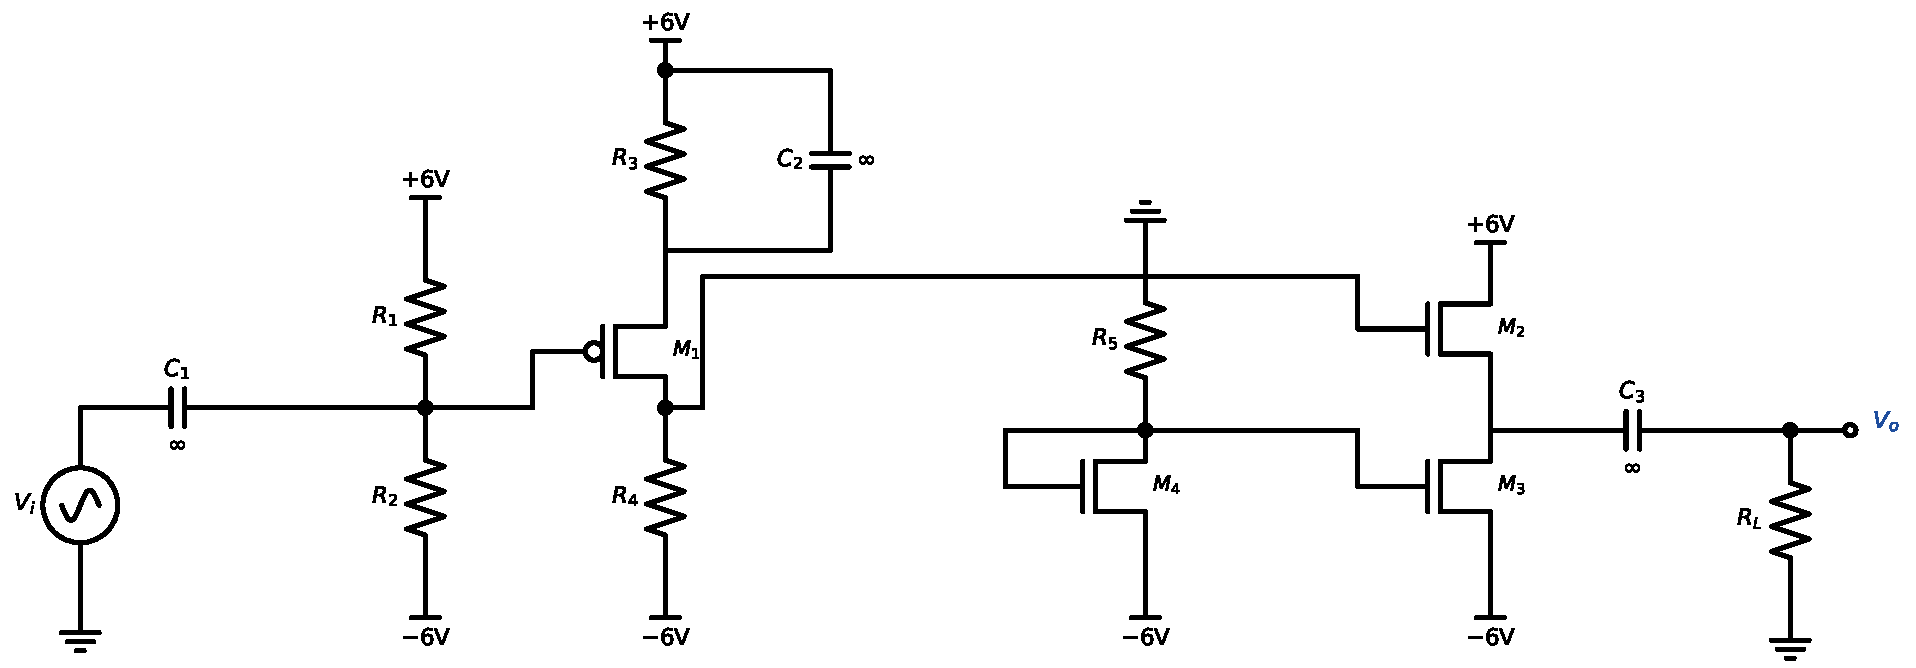
\includegraphics[width=\linewidth,height=6cm,keepaspectratio]{p08_circuit}\end{center}
\end{probbox}

\begin{probbox}{Problem 5E.9 \hfill Medium}
Design the amplifier below (find all resistor values) for the specifications in the table. Assume $k'_n\frac{W}{L} = 2\,\mathrm{m}\mathrm{A/V^2}$, $V_{tn} = 1$\,V, $k'_p\frac{W}{L} = 40\,\mathrm{m}\mathrm{A/V^2}$, $V_{tp} = -1.5$\,V; $M_2$, $M_3$ (and $M_4$) have the same $k$, $r_o = \infty$; capacitors marked $\infty$ are shorts at the signal frequency. Design choices: $I_{D3} = 20\,\mathrm{m}\mathrm{A}$; $V_{R3}$ at its minimum and $V_{R4}$ at the next multiple of 0.5\,V above its lower bound.\begin{center}\small\renewcommand{\arraystretch}{1.35}
\begin{tabular}{ll}
\toprule
specification & value \\
\midrule
Dual supply voltage & $+5$\,V / $-5$\,V \\
Load resistance $R_L$ & $100\,\Omega$ \\
0-to-peak output swing $\hat V_o$ & $\ge 1.5$\,V \\
Voltage gain $|A_v|$ & $25$ \\
Input resistance $R_i$ & $\ge 50\,\mathrm{k}\Omega$ \\
THD at $\hat V_o = 1.5$\,V & $\le 10\,\%$ \\
DC voltage drop on $R_3$ & $\ge 0.5$\,V \\
\bottomrule
\end{tabular}\end{center}

\begin{center}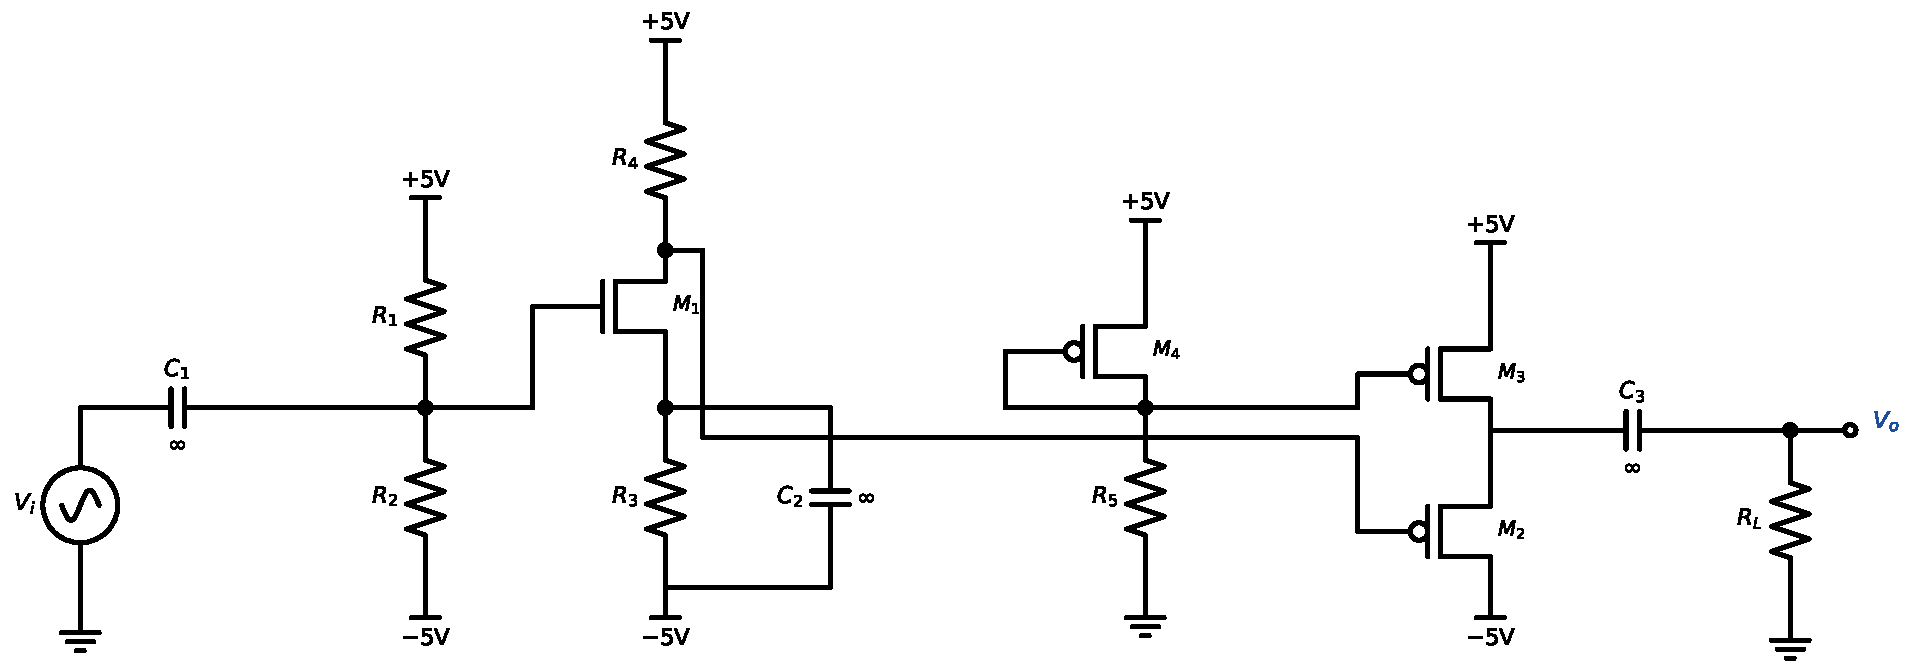
\includegraphics[width=\linewidth,height=6cm,keepaspectratio]{p09_circuit}\end{center}
\end{probbox}

\begin{probbox}{Problem 5E.10 \hfill Medium}
Design the amplifier below (find all resistor values) for the specifications in the table. Assume $k'_n\frac{W}{L} = 50\,\mathrm{m}\mathrm{A/V^2}$, $V_{tn} = 2$\,V, $k'_p\frac{W}{L} = 1\,\mathrm{m}\mathrm{A/V^2}$, $V_{tp} = -1$\,V; $M_2$, $M_3$ (and $M_4$) have the same $k$, $r_o = \infty$; capacitors marked $\infty$ are shorts at the signal frequency. Design choices: $I_{D3} = 25\,\mathrm{m}\mathrm{A}$; $V_{R3}$ at its minimum and $V_{R4}$ at the next multiple of 0.5\,V above its lower bound.\begin{center}\small\renewcommand{\arraystretch}{1.35}
\begin{tabular}{ll}
\toprule
specification & value \\
\midrule
Dual supply voltage & $+5$\,V / $-5$\,V \\
Load resistance $R_L$ & $50\,\Omega$ \\
0-to-peak output swing $\hat V_o$ & $\ge 1$\,V \\
Voltage gain $|A_v|$ & $15$ \\
Input resistance $R_i$ & $\ge 100\,\mathrm{k}\Omega$ \\
THD at $\hat V_o = 1$\,V & $\le 10\,\%$ \\
DC voltage drop on $R_3$ & $\ge 0.5$\,V \\
\bottomrule
\end{tabular}\end{center}

\begin{center}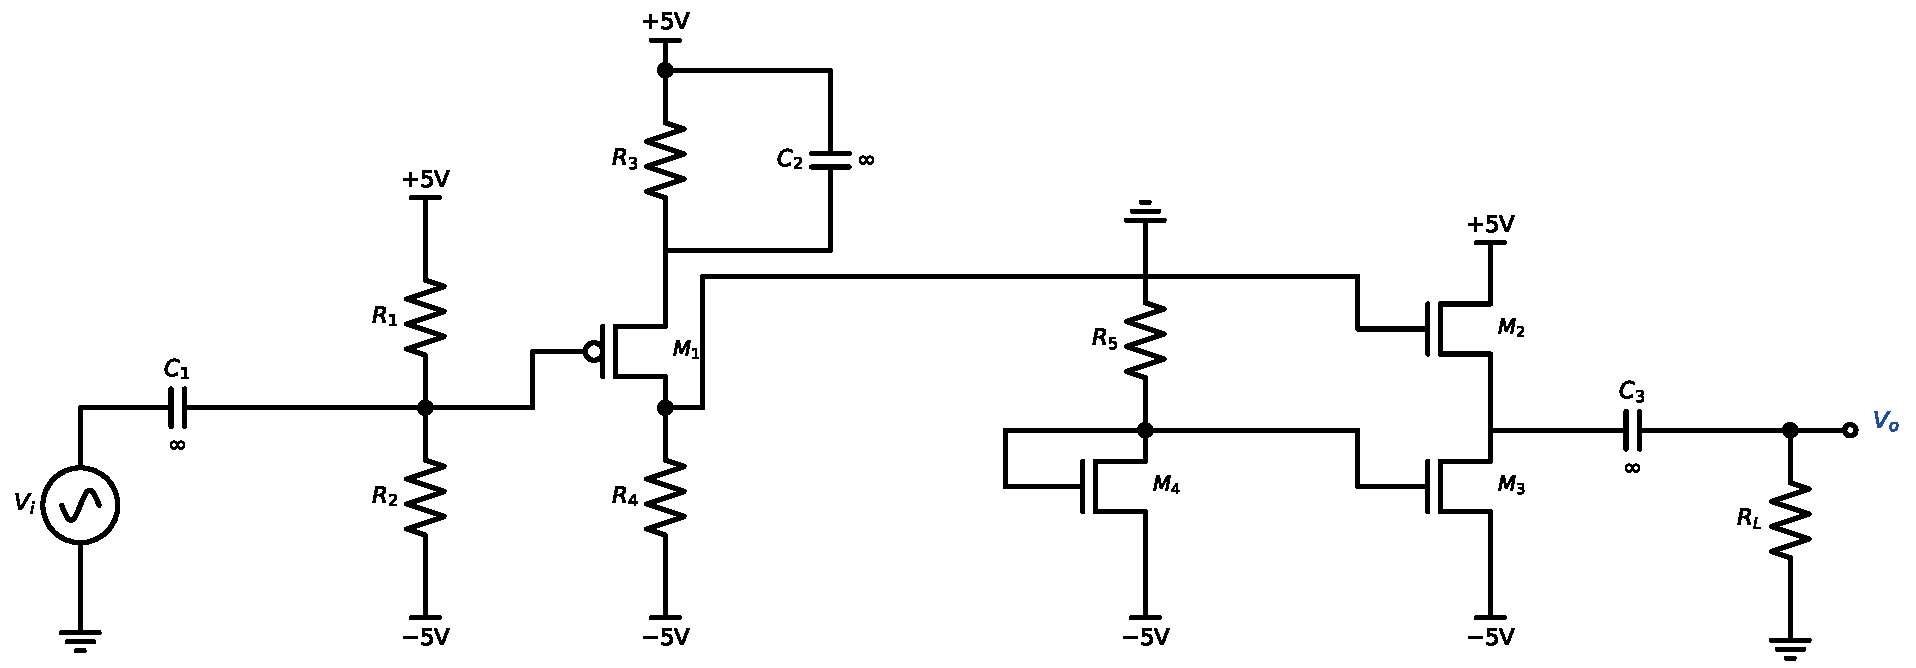
\includegraphics[width=\linewidth,height=6cm,keepaspectratio]{p10_circuit}\end{center}
\end{probbox}

\begin{probbox}{Problem 5E.11 \hfill Medium}
Design the amplifier below (find all resistor values) for the specifications in the table. Assume $k'_n\frac{W}{L} = 1\,\mathrm{m}\mathrm{A/V^2}$, $V_{tn} = 1$\,V, $k'_p\frac{W}{L} = 50\,\mathrm{m}\mathrm{A/V^2}$, $V_{tp} = -1.5$\,V; $M_2$, $M_3$ (and $M_4$) have the same $k$, $r_o = \infty$; capacitors marked $\infty$ are shorts at the signal frequency. Design choices: $I_{D3} = 12\,\mathrm{m}\mathrm{A}$; $V_{R3}$ at its minimum and $V_{R4}$ at the next multiple of 0.5\,V above its lower bound.\begin{center}\small\renewcommand{\arraystretch}{1.35}
\begin{tabular}{ll}
\toprule
specification & value \\
\midrule
Dual supply voltage & $+6$\,V / $-6$\,V \\
Load resistance $R_L$ & $200\,\Omega$ \\
0-to-peak output swing $\hat V_o$ & $\ge 2$\,V \\
Voltage gain $|A_v|$ & $20$ \\
Input resistance $R_i$ & $\ge 100\,\mathrm{k}\Omega$ \\
THD at $\hat V_o = 2$\,V & $\le 10\,\%$ \\
DC voltage drop on $R_3$ & $\ge 0.5$\,V \\
\bottomrule
\end{tabular}\end{center}

\begin{center}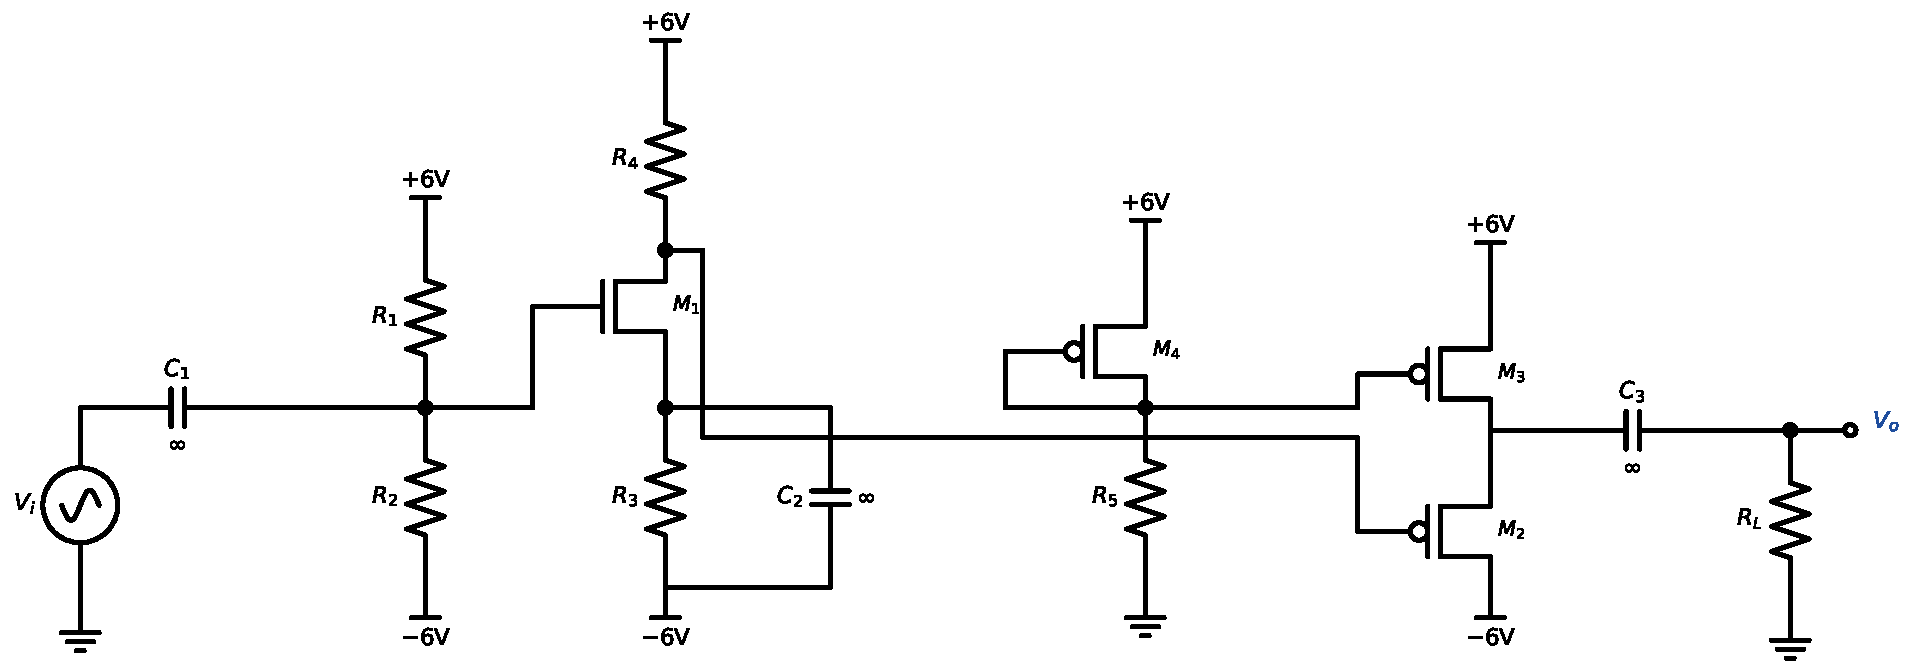
\includegraphics[width=\linewidth,height=6cm,keepaspectratio]{p11_circuit}\end{center}
\end{probbox}

\begin{probbox}{Problem 5E.12 \hfill Medium}
Design the amplifier below (find all resistor values) for the specifications in the table. Assume $k'_n\frac{W}{L}\big|_{4} = 10\,\mathrm{m}\mathrm{A/V^2}$, $k'_n\frac{W}{L}\big|_{2} = 50\,\mathrm{m}\mathrm{A/V^2}$, $k'_n\frac{W}{L}\big|_{3} = 50\,\mathrm{m}\mathrm{A/V^2}$, $V_{tn} = 2$\,V, $k'_p\frac{W}{L} = 1\,\mathrm{m}\mathrm{A/V^2}$, $V_{tp} = -1$\,V; $M_2$, $M_3$ (and $M_4$) have the same $k$, $r_o = \infty$; capacitors marked $\infty$ are shorts at the signal frequency. Design choices: $I_{D3} = 20\,\mathrm{m}\mathrm{A}$; $V_{R3}$ at its minimum and $V_{R4}$ at the next multiple of 0.5\,V above its lower bound; $M_4$ has $k_4 = 0.2\,k_3$.\begin{center}\small\renewcommand{\arraystretch}{1.35}
\begin{tabular}{ll}
\toprule
specification & value \\
\midrule
Dual supply voltage & $+5$\,V / $-5$\,V \\
Load resistance $R_L$ & $100\,\Omega$ \\
0-to-peak output swing $\hat V_o$ & $\ge 1.5$\,V \\
Voltage gain $|A_v|$ & $30$ \\
Input resistance $R_i$ & $\ge 100\,\mathrm{k}\Omega$ \\
THD at $\hat V_o = 1.5$\,V & $\le 10\,\%$ \\
DC voltage drop on $R_3$ & $\ge 0.5$\,V \\
\bottomrule
\end{tabular}\end{center}

\begin{center}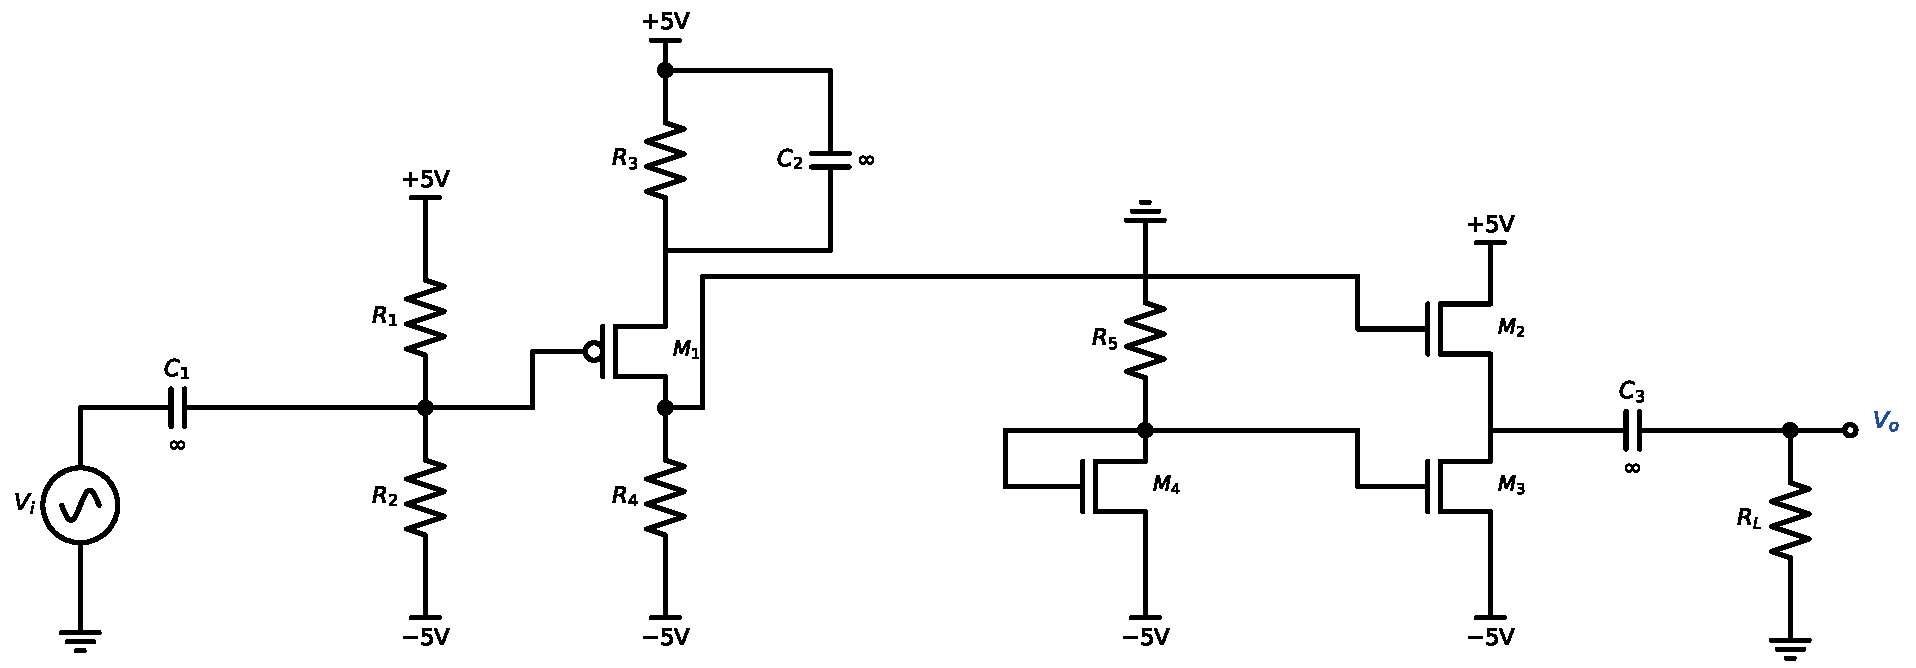
\includegraphics[width=\linewidth,height=6cm,keepaspectratio]{p12_circuit}\end{center}
\end{probbox}

\subsection*{Hard problems}
\begin{probbox}{Problem 5E.13 \hfill Hard}
Design the amplifier below (find all resistor values) for the specifications in the table. Assume $k'_n\frac{W}{L} = 50\,\mathrm{m}\mathrm{A/V^2}$, $V_{tn} = 2$\,V, $k'_p\frac{W}{L} = 1\,\mathrm{m}\mathrm{A/V^2}$, $V_{tp} = -1$\,V; $M_2$, $M_3$ (and $M_4$) have the same $k$, $r_o = \infty$; capacitors marked $\infty$ are shorts at the signal frequency. Design choices: $I_{D3} = 25\,\mathrm{m}\mathrm{A}$; $V_{R3}$ at its minimum and $V_{R4}$ at the next multiple of 0.5\,V above its lower bound. (These are the specifications of Sample Problem 5.)\begin{center}\small\renewcommand{\arraystretch}{1.35}
\begin{tabular}{ll}
\toprule
specification & value \\
\midrule
Dual supply voltage & $+5$\,V / $-5$\,V \\
Load resistance $R_L$ & $100\,\Omega$ \\
0-to-peak output swing $\hat V_o$ & $\ge 2$\,V \\
Voltage gain $|A_v|$ & $40$ \\
Input resistance $R_i$ & $\ge 50\,\mathrm{k}\Omega$ \\
THD at $\hat V_o = 2$\,V & $\le 10\,\%$ \\
DC voltage drop on $R_3$ & $\ge 0.5$\,V \\
\bottomrule
\end{tabular}\end{center}

\begin{center}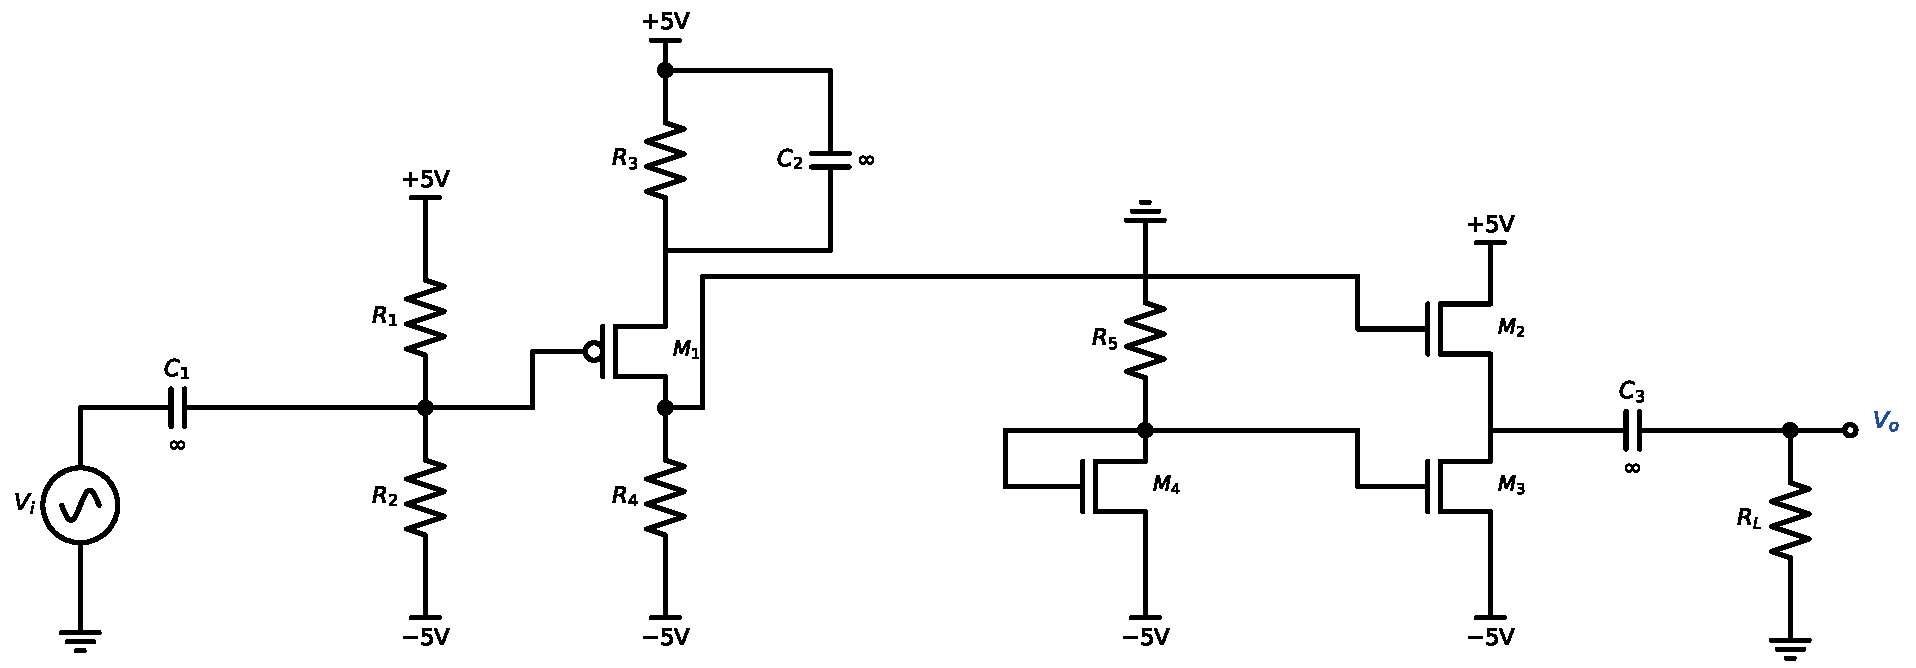
\includegraphics[width=\linewidth,height=6cm,keepaspectratio]{p13_circuit}\end{center}
\end{probbox}

\begin{probbox}{Problem 5E.14 \hfill Hard}
Design the amplifier below (find all resistor values) for the specifications in the table. Assume $k'_n\frac{W}{L} = 1\,\mathrm{m}\mathrm{A/V^2}$, $V_{tn} = 1$\,V, $k'_p\frac{W}{L} = 50\,\mathrm{m}\mathrm{A/V^2}$, $V_{tp} = -2$\,V; $M_2$, $M_3$ (and $M_4$) have the same $k$, $r_o = \infty$; capacitors marked $\infty$ are shorts at the signal frequency. Design choices: $I_{D3} = 25\,\mathrm{m}\mathrm{A}$; $V_{R3}$ at its minimum and $V_{R4}$ at the next multiple of 0.5\,V above its lower bound.\begin{center}\small\renewcommand{\arraystretch}{1.35}
\begin{tabular}{ll}
\toprule
specification & value \\
\midrule
Dual supply voltage & $+5$\,V / $-5$\,V \\
Load resistance $R_L$ & $100\,\Omega$ \\
0-to-peak output swing $\hat V_o$ & $\ge 2$\,V \\
Voltage gain $|A_v|$ & $40$ \\
Input resistance $R_i$ & $\ge 50\,\mathrm{k}\Omega$ \\
THD at $\hat V_o = 2$\,V & $\le 10\,\%$ \\
DC voltage drop on $R_3$ & $\ge 0.5$\,V \\
\bottomrule
\end{tabular}\end{center}

\begin{center}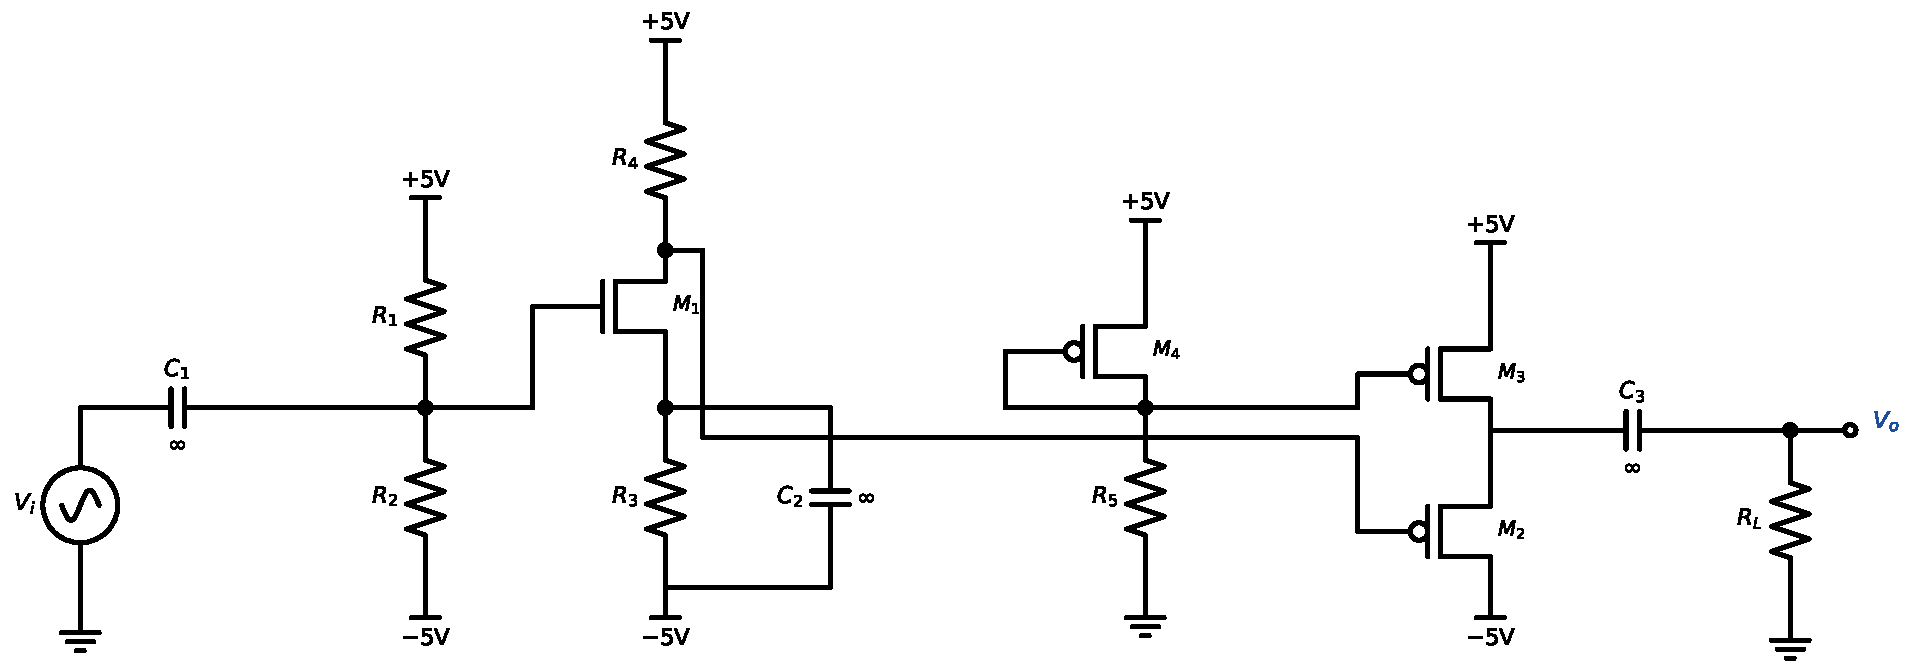
\includegraphics[width=\linewidth,height=6cm,keepaspectratio]{p14_circuit}\end{center}
\end{probbox}

\begin{probbox}{Problem 5E.15 \hfill Hard}
Design the amplifier below (find all resistor values) for the specifications in the table. Assume $k'_n\frac{W}{L} = 50\,\mathrm{m}\mathrm{A/V^2}$, $V_{tn} = 2$\,V, $k'_p\frac{W}{L} = 1\,\mathrm{m}\mathrm{A/V^2}$, $V_{tp} = -1$\,V; $M_2$, $M_3$ (and $M_4$) have the same $k$, $r_o = \infty$; capacitors marked $\infty$ are shorts at the signal frequency. Design choices: $I_{D3} = 45\,\mathrm{m}\mathrm{A}$; $V_{R3}$ at its minimum and $V_{R4}$ at the next multiple of 0.5\,V above its lower bound.\begin{center}\small\renewcommand{\arraystretch}{1.35}
\begin{tabular}{ll}
\toprule
specification & value \\
\midrule
Dual supply voltage & $+9$\,V / $-9$\,V \\
Load resistance $R_L$ & $100\,\Omega$ \\
0-to-peak output swing $\hat V_o$ & $\ge 4$\,V \\
Voltage gain $|A_v|$ & $50$ \\
Input resistance $R_i$ & $\ge 100\,\mathrm{k}\Omega$ \\
THD at $\hat V_o = 4$\,V & $\le 10\,\%$ \\
DC voltage drop on $R_3$ & $\ge 1$\,V \\
\bottomrule
\end{tabular}\end{center}

\begin{center}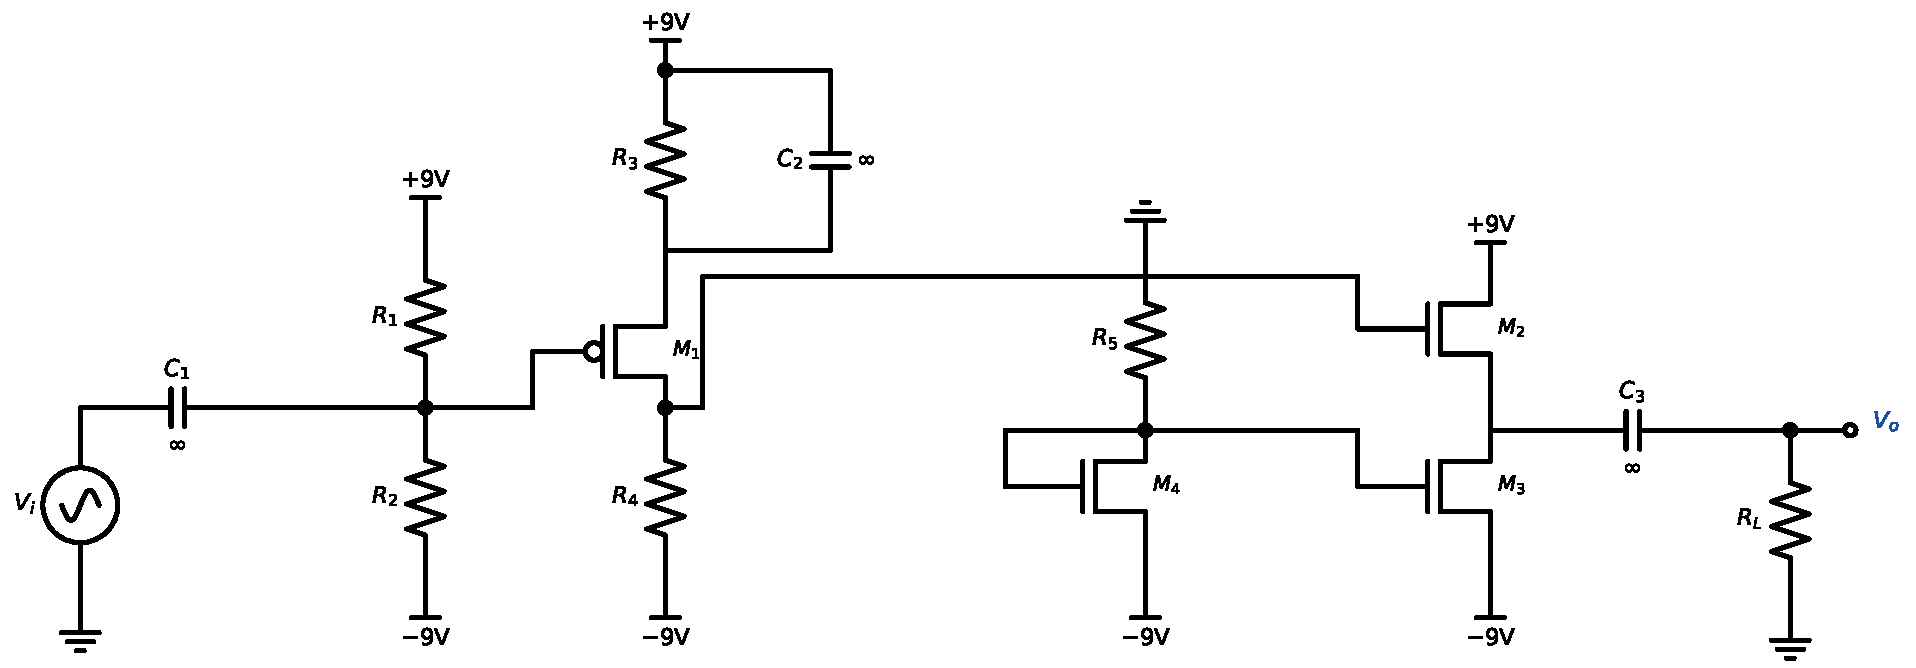
\includegraphics[width=\linewidth,height=6cm,keepaspectratio]{p15_circuit}\end{center}
\end{probbox}

\begin{probbox}{Problem 5E.16 \hfill Hard}
Design the amplifier below (find all resistor values) for the specifications in the table. Assume $k'_n\frac{W}{L} = 2\,\mathrm{m}\mathrm{A/V^2}$, $V_{tn} = 0.8$\,V, $k'_p\frac{W}{L}\big|_{4} = 15\,\mathrm{m}\mathrm{A/V^2}$, $k'_p\frac{W}{L}\big|_{3} = 60\,\mathrm{m}\mathrm{A/V^2}$, $k'_p\frac{W}{L}\big|_{2} = 60\,\mathrm{m}\mathrm{A/V^2}$, $V_{tp} = -1.2$\,V; $M_2$, $M_3$ (and $M_4$) have the same $k$, $r_o = \infty$; capacitors marked $\infty$ are shorts at the signal frequency. Design choices: $I_{D3} = 35\,\mathrm{m}\mathrm{A}$; $V_{R3}$ at its minimum and $V_{R4}$ at the next multiple of 0.5\,V above its lower bound; $M_4$ has $k_4 = 0.25\,k_3$.\begin{center}\small\renewcommand{\arraystretch}{1.35}
\begin{tabular}{ll}
\toprule
specification & value \\
\midrule
Dual supply voltage & $+5$\,V / $-5$\,V \\
Load resistance $R_L$ & $50\,\Omega$ \\
0-to-peak output swing $\hat V_o$ & $\ge 1.5$\,V \\
Voltage gain $|A_v|$ & $30$ \\
Input resistance $R_i$ & $\ge 200\,\mathrm{k}\Omega$ \\
THD at $\hat V_o = 1.5$\,V & $\le 8\,\%$ \\
DC voltage drop on $R_3$ & $\ge 0.5$\,V \\
\bottomrule
\end{tabular}\end{center}

\begin{center}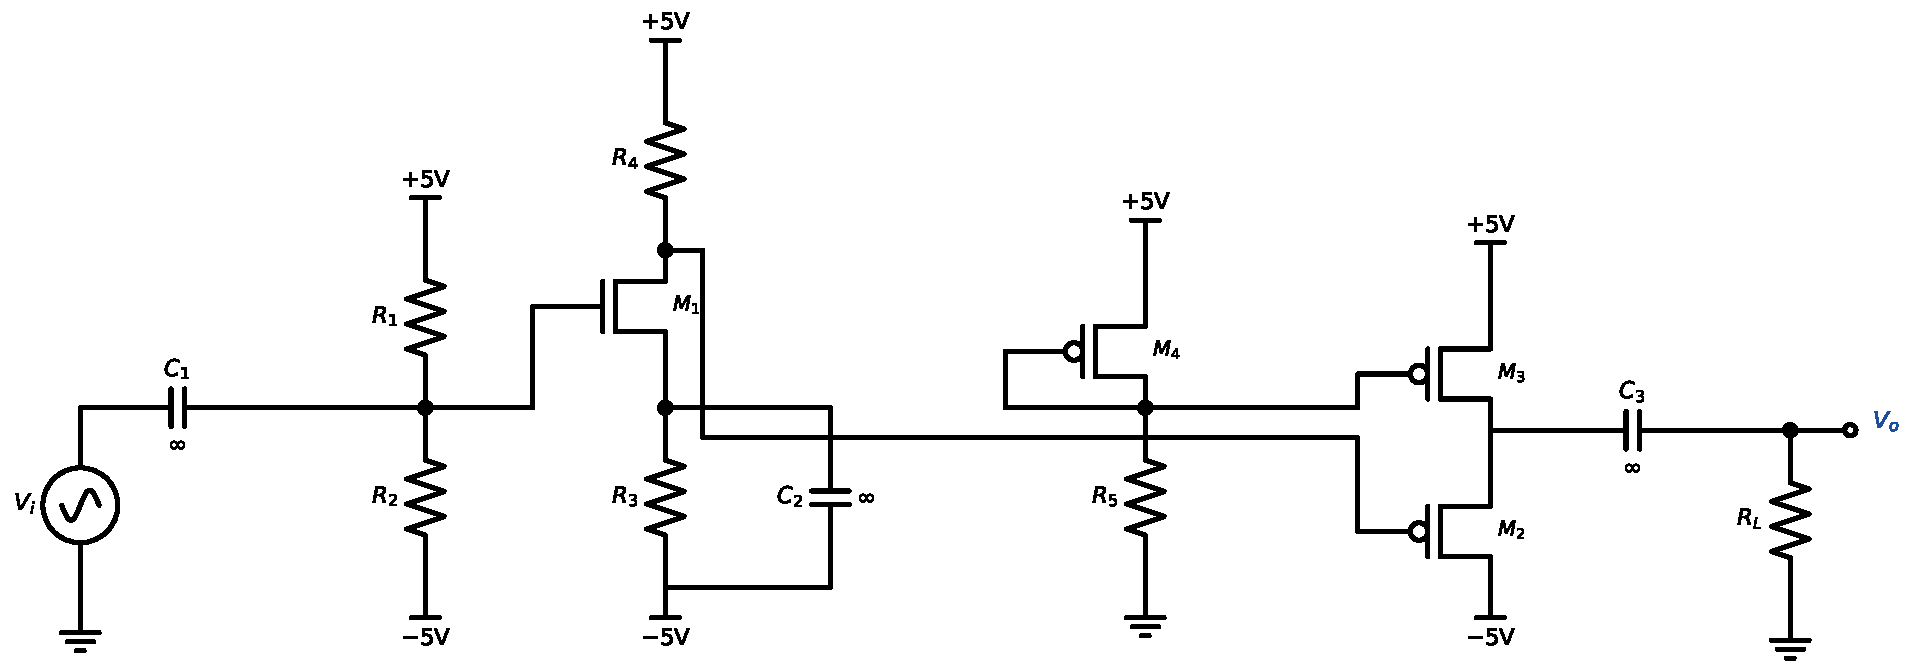
\includegraphics[width=\linewidth,height=6cm,keepaspectratio]{p16_circuit}\end{center}
\end{probbox}

\begin{probbox}{Problem 5E.17 \hfill Hard}
Design the amplifier below (find all resistor values) for the specifications in the table. Assume $k'_n\frac{W}{L}\big|_{4} = 25\,\mathrm{m}\mathrm{A/V^2}$, $k'_n\frac{W}{L}\big|_{2} = 50\,\mathrm{m}\mathrm{A/V^2}$, $k'_n\frac{W}{L}\big|_{3} = 50\,\mathrm{m}\mathrm{A/V^2}$, $V_{tn} = 2$\,V, $k'_p\frac{W}{L} = 1\,\mathrm{m}\mathrm{A/V^2}$, $V_{tp} = -1$\,V; $M_2$, $M_3$ (and $M_4$) have the same $k$, $r_o = \infty$; capacitors marked $\infty$ are shorts at the signal frequency. Design choices: $I_{D3} = 30\,\mathrm{m}\mathrm{A}$; $V_{R3}$ at its minimum and $V_{R4}$ at the next multiple of 0.5\,V above its lower bound; $M_4$ has $k_4 = 0.5\,k_3$.\begin{center}\small\renewcommand{\arraystretch}{1.35}
\begin{tabular}{ll}
\toprule
specification & value \\
\midrule
Dual supply voltage & $+6$\,V / $-6$\,V \\
Load resistance $R_L$ & $75\,\Omega$ \\
0-to-peak output swing $\hat V_o$ & $\ge 2$\,V \\
Voltage gain $|A_v|$ & $60$ \\
Input resistance $R_i$ & $\ge 100\,\mathrm{k}\Omega$ \\
THD at $\hat V_o = 2$\,V & $\le 10\,\%$ \\
DC voltage drop on $R_3$ & $\ge 0.5$\,V \\
\bottomrule
\end{tabular}\end{center}

\begin{center}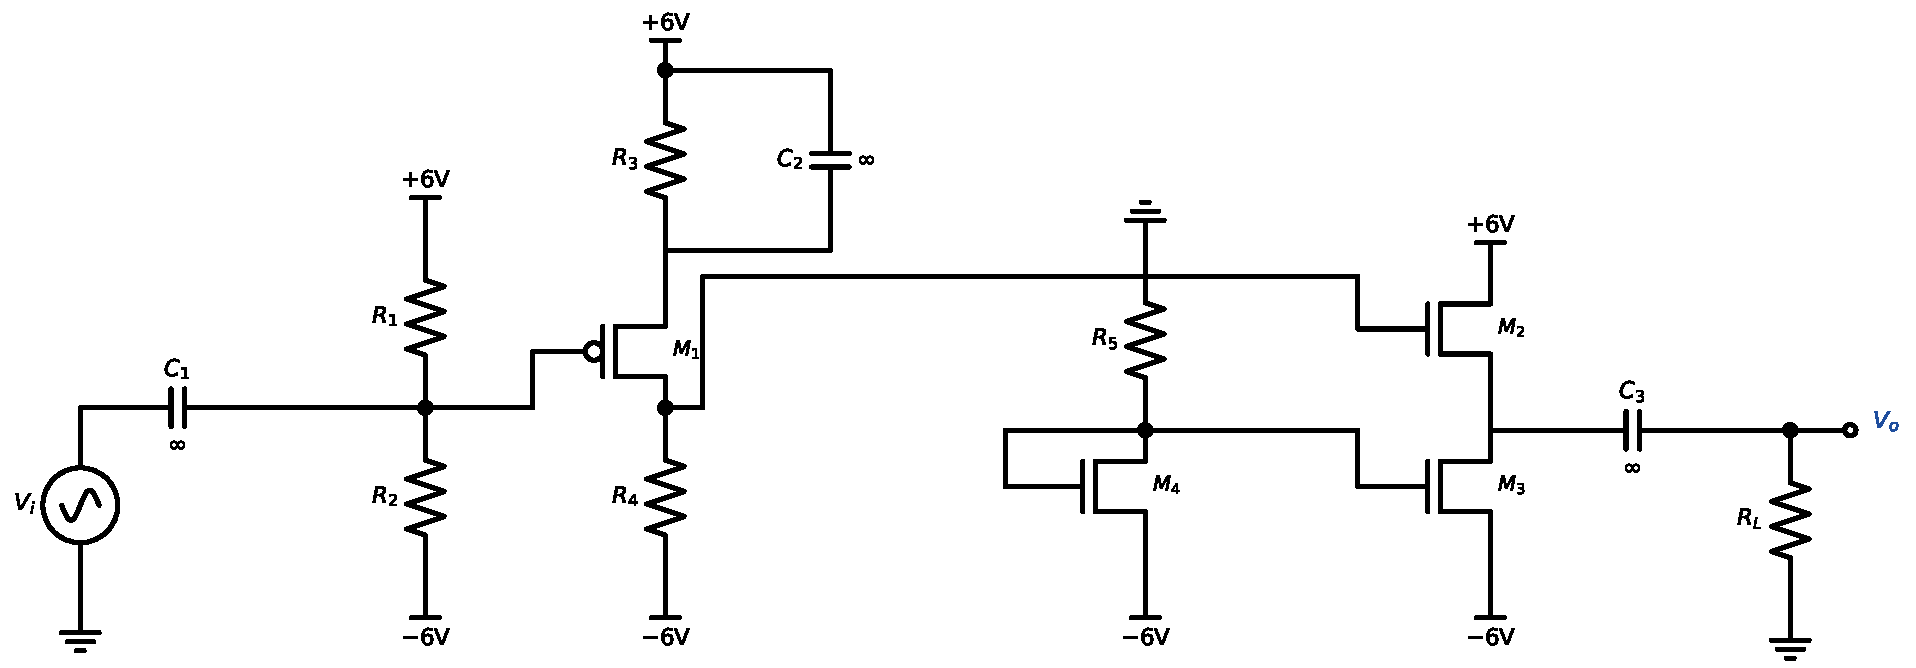
\includegraphics[width=\linewidth,height=6cm,keepaspectratio]{p17_circuit}\end{center}
\end{probbox}

\begin{probbox}{Problem 5E.18 \hfill Hard}
Design the amplifier below (find all resistor values) for the specifications in the table. Assume $k'_n\frac{W}{L} = 1\,\mathrm{m}\mathrm{A/V^2}$, $V_{tn} = 0.7$\,V, $k'_p\frac{W}{L} = 50\,\mathrm{m}\mathrm{A/V^2}$, $V_{tp} = -1$\,V; $M_2$, $M_3$ (and $M_4$) have the same $k$, $r_o = \infty$; capacitors marked $\infty$ are shorts at the signal frequency. Design choices: $I_{D3} = 12\,\mathrm{m}\mathrm{A}$; $V_{R3}$ at its minimum and $V_{R4}$ at the next multiple of 0.5\,V above its lower bound.\begin{center}\small\renewcommand{\arraystretch}{1.35}
\begin{tabular}{ll}
\toprule
specification & value \\
\midrule
Dual supply voltage & $+4$\,V / $-4$\,V \\
Load resistance $R_L$ & $100\,\Omega$ \\
0-to-peak output swing $\hat V_o$ & $\ge 1$\,V \\
Voltage gain $|A_v|$ & $20$ \\
Input resistance $R_i$ & $\ge 50\,\mathrm{k}\Omega$ \\
THD at $\hat V_o = 1$\,V & $\le 10\,\%$ \\
DC voltage drop on $R_3$ & $\ge 0.5$\,V \\
\bottomrule
\end{tabular}\end{center}

\begin{center}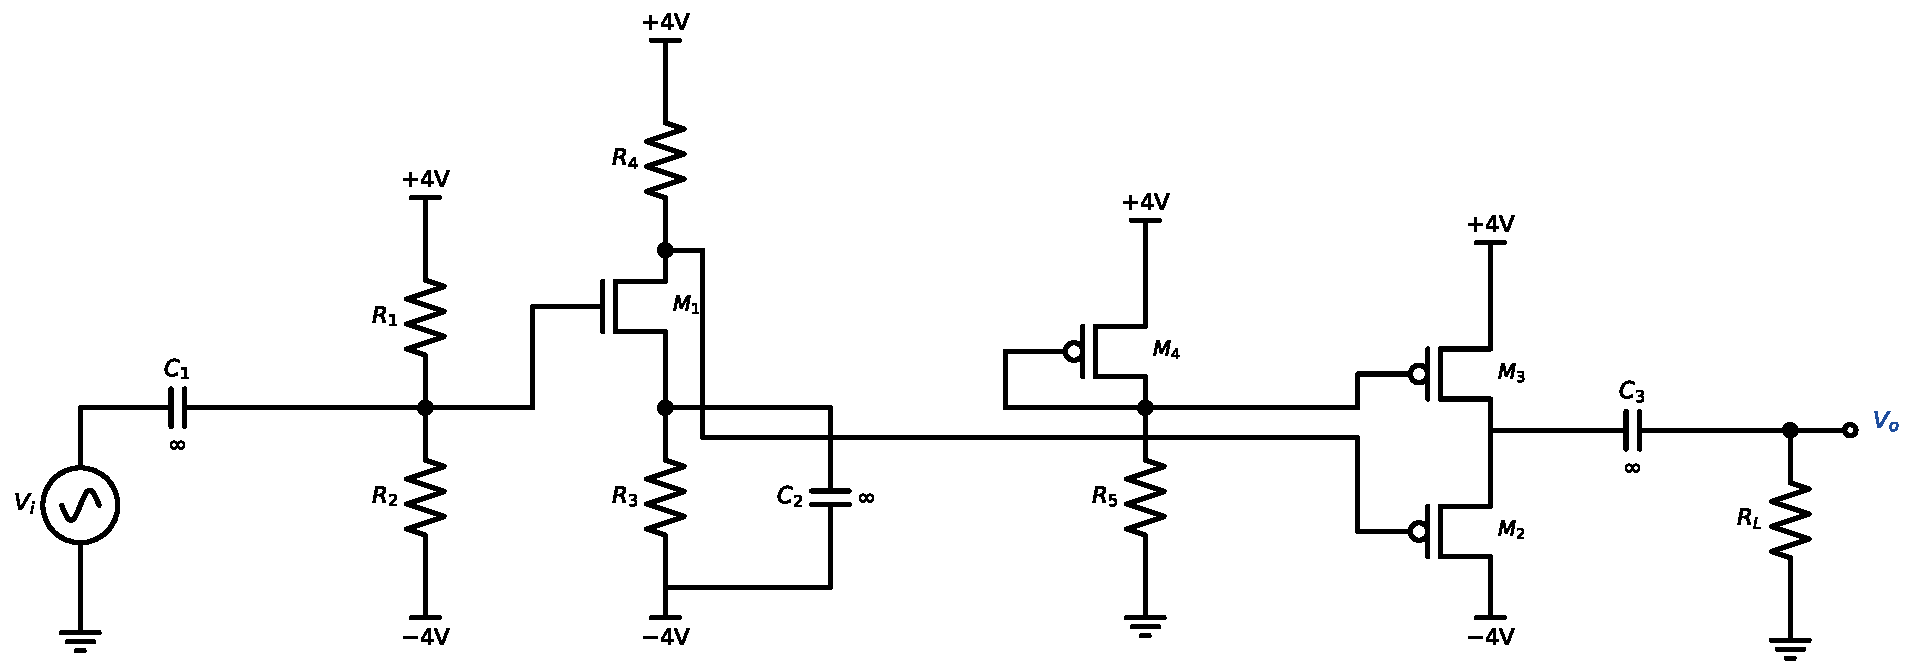
\includegraphics[width=\linewidth,height=6cm,keepaspectratio]{p18_circuit}\end{center}
\end{probbox}

\newpage
\section*{Solutions}
Every solution follows the steps of the Lecture-5 pipeline card.
\subsection*{Solution 5E.1 \hfill Easy}
\begin{center}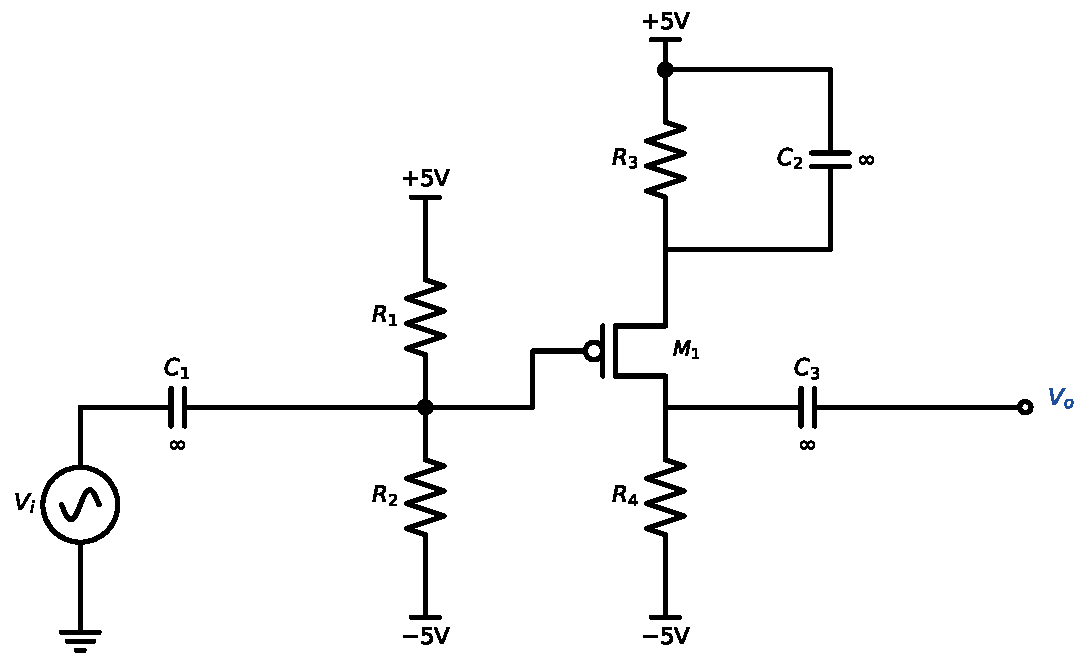
\includegraphics[width=0.9\linewidth,height=6cm,keepaspectratio]{p01_circuit}\end{center}
\solstep{1}{Plan}Follow the procedure of Sample Problem 5: budget the supply voltage around the drain swing; get $V_{ov1}$ from the gain ($|A_v| = g_mR = 2V_R/V_{ov}$), then the resistors; finally the gate divider from the input resistance. Distortion of a common-source stage: $HD_2 \approx \frac{\hat v_{gs}}{4V_{ov}}$ (from $i_D = \frac{k}{2}(V_{ov} + v_{gs})^2$).
\solstep{2}{Design of the stage}Voltage budget of the $V_{DD} + V_{SS} = 10$\,V branch through $R_3$, $M_1$, $R_4$. At its extreme the drain cannot pass the supply on the $R_4$ side: \[V_{R4} \ge \hat V_o = 2\,\mathrm{V}\]$M_1$ must stay active at the other extreme: $V_{R3} + V_{ov1} + \hat V_d + V_{R4} \le 10$, and with $V_{ov1} = 2V_{R4}/|A_{v1}|$ (below): \[V_{R4}\left(1 + \frac{2}{|A_{v1}|}\right) \le 10 - V_{R3} - \hat V_d \Rightarrow V_{R4} \le 6.818\,\mathrm{V}\]$V_{R3} = 0.5$\,V (its minimum) and $V_{R4} = 5$\,V (given).

Gain of the common-source stage ($R_3$ is bypassed, the follower's gate loads nothing): \[|A_{v1}| = g_{m1}R_4 = k_1V_{ov1}\frac{V_{R4}}{\frac{k_1}{2}V_{ov1}^2} = \frac{2V_{R4}}{V_{ov1}} \Rightarrow V_{ov1} = \frac{2\cdot5}{20} = 0.5\,\mathrm{V}\]$I_{D1} = \frac{k_1}{2}V_{ov1}^2 = 125\,\mu \mathrm{A}$, $R_4 = \frac{V_{R4}}{I_{D1}} = \mathbf{40\,\mathrm{k}\Omega}$, $R_3 = \frac{V_{R3}}{I_{D1}} = \mathbf{4\,\mathrm{k}\Omega}$.

Gate divider: the resistor on the source side of $M_1$ carries $V_{R1} = V_{R3} + |V_{t1}| + V_{ov1} = 2$\,V, the other one $V_{R2} = 10 - 2 = 8$\,V. Both carry the same current ($I_G = 0$): $R_{1} = 2X$, $R_{2} = 8X$, and the input resistance is their parallel combination: \[R_1\|R_2 = \frac{2\cdot8}{10}X \ge 100\,\mathrm{k}\Omega \Rightarrow X = 62.5\,\mathrm{k}\Omega:\quad \mathbf{R_1 = 125\,\mathrm{k}\Omega},\ \mathbf{R_2 = 500\,\mathrm{k}\Omega}\]
\solstep{3}{Check by analysis}DC analysis of the finished circuit (as in sets 5A/5B):\begin{center}\renewcommand{\arraystretch}{1.35}
\begin{tabular}{cccc}
\toprule
 & $I_D$ & $V_{ov}$ & $|V_{DS}|$ \\
\midrule
$M_{1}$ & $125\,\mu \mathrm{A}$ & $0.5$\,V & $4.5$\,V \\
\bottomrule
\end{tabular}\end{center}
\begin{itemize}[leftmargin=*,itemsep=2pt]
\item $V_{SD1} = V_{S1} - V_{D1} = 4.5 - (-8.674\times 10^{-15}) = 4.5\,\mathrm{V}$ $\ge V_{ov1} = 0.5$\,V $\Rightarrow$ $M_{1}$ is active \checkmark
\item Gain (exact small-signal analysis of the finished circuit): $|A_v| = 20$ \checkmark
\item Input resistance $R_1\|R_2 = 100\,\mathrm{k}\Omega \ge 100\,\mathrm{k}\Omega$ \checkmark
\item Output swing before clipping: $M_1$ leaves saturation at $\hat V_o = 4$\,V; the drain reaches the supply at $\hat V_o = 5$\,V. The smallest is $4$\,V $\ge 2$\,V \checkmark
\item THD $\approx HD_2 = \frac{\hat v_{gs1}}{4V_{ov1}} = \frac{2/20}{4\cdot0.5} = 5\,\%$ $\le 6\,\%$ \checkmark
\end{itemize}

\begin{center}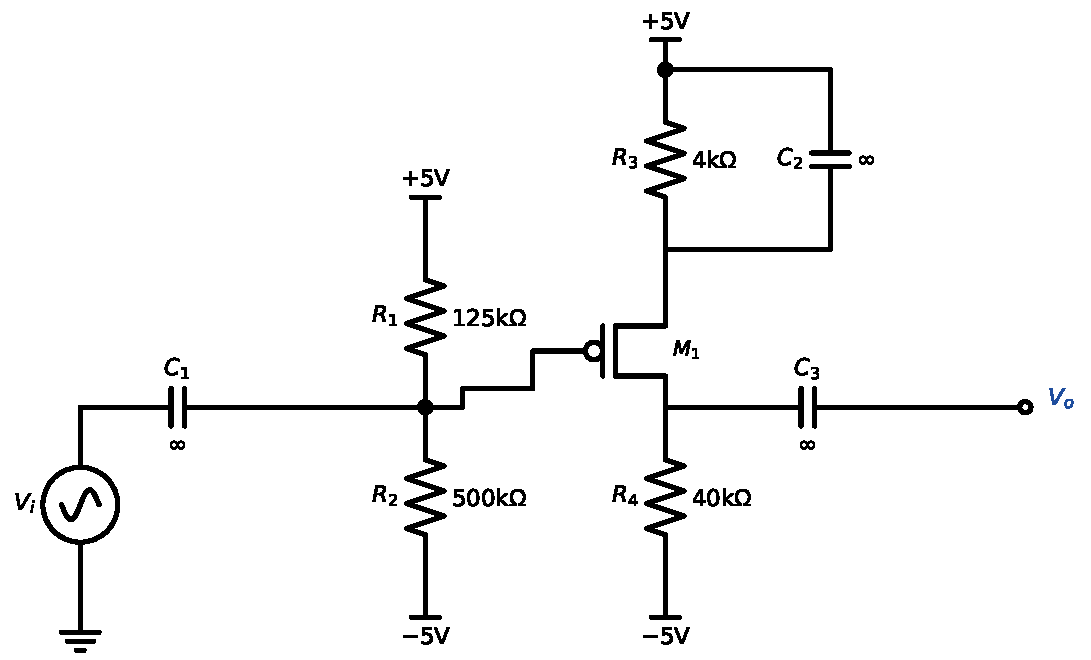
\includegraphics[width=0.85\linewidth,height=6cm,keepaspectratio]{p01_designed}\end{center}

\begin{ansbox}
$R_{1} = 125\,\mathrm{k}\Omega$,\quad $R_{2} = 500\,\mathrm{k}\Omega$,\quad $R_{3} = 4\,\mathrm{k}\Omega$,\quad $R_{4} = 40\,\mathrm{k}\Omega$
\end{ansbox}

\newpage
\subsection*{Solution 5E.2 \hfill Easy}
\begin{center}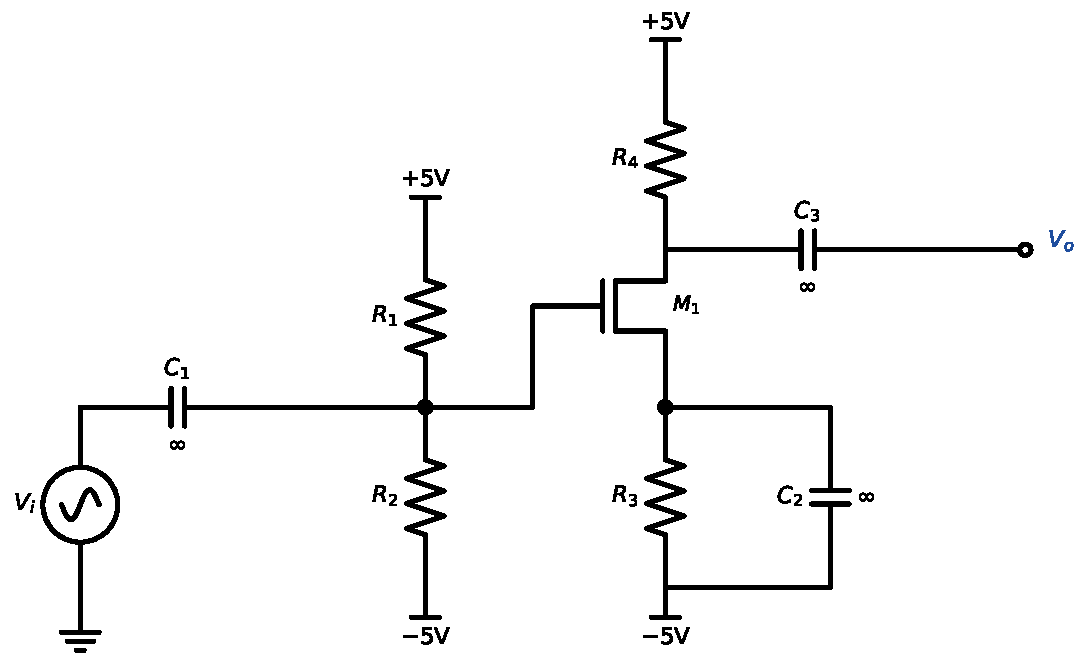
\includegraphics[width=0.9\linewidth,height=6cm,keepaspectratio]{p02_circuit}\end{center}
\solstep{1}{Plan}Follow the procedure of Sample Problem 5: budget the supply voltage around the drain swing; get $V_{ov1}$ from the gain ($|A_v| = g_mR = 2V_R/V_{ov}$), then the resistors; finally the gate divider from the input resistance. Distortion of a common-source stage: $HD_2 \approx \frac{\hat v_{gs}}{4V_{ov}}$ (from $i_D = \frac{k}{2}(V_{ov} + v_{gs})^2$).
\solstep{2}{Design of the stage}Voltage budget of the $V_{DD} + V_{SS} = 10$\,V branch through $R_3$, $M_1$, $R_4$. At its extreme the drain cannot pass the supply on the $R_4$ side: \[V_{R4} \ge \hat V_o = 1.5\,\mathrm{V}\]$M_1$ must stay active at the other extreme: $V_{R3} + V_{ov1} + \hat V_d + V_{R4} \le 10$, and with $V_{ov1} = 2V_{R4}/|A_{v1}|$ (below): \[V_{R4}\left(1 + \frac{2}{|A_{v1}|}\right) \le 10 - V_{R3} - \hat V_d \Rightarrow V_{R4} \le 6.944\,\mathrm{V}\]$V_{R3} = 1$\,V (its minimum) and $V_{R4} = 5$\,V (given).

Gain of the common-source stage ($R_3$ is bypassed, the follower's gate loads nothing): \[|A_{v1}| = g_{m1}R_4 = k_1V_{ov1}\frac{V_{R4}}{\frac{k_1}{2}V_{ov1}^2} = \frac{2V_{R4}}{V_{ov1}} \Rightarrow V_{ov1} = \frac{2\cdot5}{25} = 0.4\,\mathrm{V}\]$I_{D1} = \frac{k_1}{2}V_{ov1}^2 = 80\,\mu \mathrm{A}$, $R_4 = \frac{V_{R4}}{I_{D1}} = \mathbf{62.5\,\mathrm{k}\Omega}$, $R_3 = \frac{V_{R3}}{I_{D1}} = \mathbf{12.5\,\mathrm{k}\Omega}$.

Gate divider: the resistor on the source side of $M_1$ carries $V_{R2} = V_{R3} + |V_{t1}| + V_{ov1} = 2.4$\,V, the other one $V_{R1} = 10 - 2.4 = 7.6$\,V. Both carry the same current ($I_G = 0$): $R_{2} = 2.4X$, $R_{1} = 7.6X$, and the input resistance is their parallel combination: \[R_1\|R_2 = \frac{2.4\cdot7.6}{10}X \ge 200\,\mathrm{k}\Omega \Rightarrow X = 110\,\mathrm{k}\Omega:\quad \mathbf{R_1 = 833\,\mathrm{k}\Omega},\ \mathbf{R_2 = 263\,\mathrm{k}\Omega}\]
\solstep{3}{Check by analysis}DC analysis of the finished circuit (as in sets 5A/5B):\begin{center}\renewcommand{\arraystretch}{1.35}
\begin{tabular}{cccc}
\toprule
 & $I_D$ & $V_{ov}$ & $|V_{DS}|$ \\
\midrule
$M_{1}$ & $80\,\mu \mathrm{A}$ & $0.4$\,V & $4$\,V \\
\bottomrule
\end{tabular}\end{center}
\begin{itemize}[leftmargin=*,itemsep=2pt]
\item $V_{DS1} = V_{D1} - V_{S1} = -2.541\times 10^{-15} - (-4) = 4\,\mathrm{V}$ $\ge V_{ov1} = 0.4$\,V $\Rightarrow$ $M_{1}$ is active \checkmark
\item Gain (exact small-signal analysis of the finished circuit): $|A_v| = 25$ \checkmark
\item Input resistance $R_1\|R_2 = 200\,\mathrm{k}\Omega \ge 200\,\mathrm{k}\Omega$ \checkmark
\item Output swing before clipping: $M_1$ leaves saturation at $\hat V_o = 3.6$\,V; the drain reaches the supply at $\hat V_o = 5$\,V. The smallest is $3.6$\,V $\ge 1.5$\,V \checkmark
\item THD $\approx HD_2 = \frac{\hat v_{gs1}}{4V_{ov1}} = \frac{1.5/25}{4\cdot0.4} = 3.7\,\%$ $\le 5\,\%$ \checkmark
\end{itemize}

\begin{center}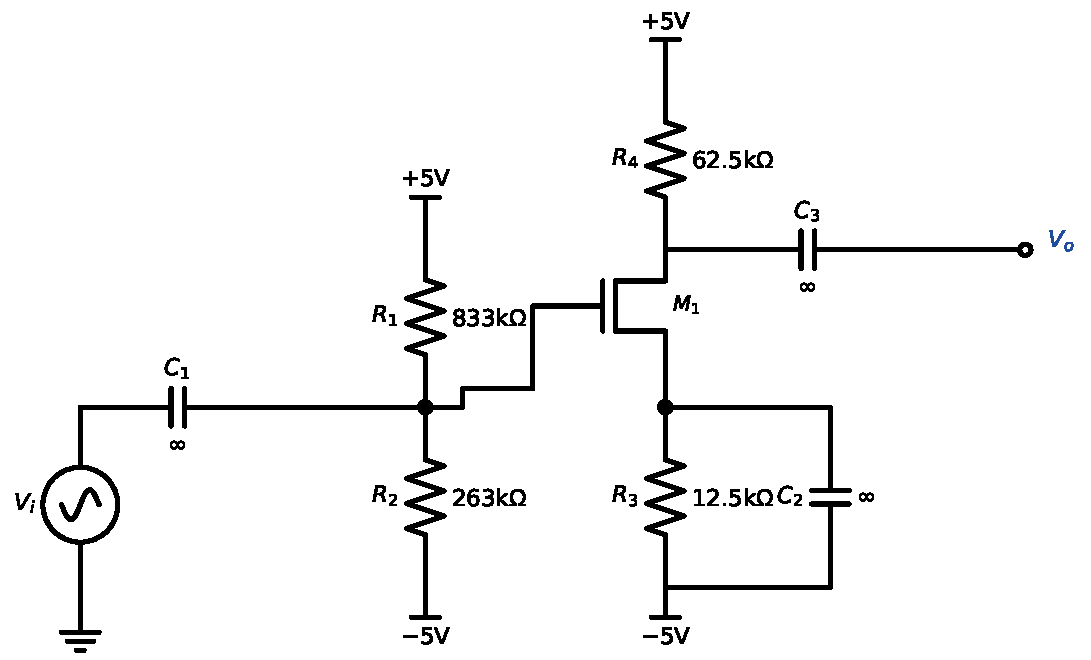
\includegraphics[width=0.85\linewidth,height=6cm,keepaspectratio]{p02_designed}\end{center}

\begin{ansbox}
$R_{1} = 833\,\mathrm{k}\Omega$,\quad $R_{2} = 263\,\mathrm{k}\Omega$,\quad $R_{3} = 12.5\,\mathrm{k}\Omega$,\quad $R_{4} = 62.5\,\mathrm{k}\Omega$
\end{ansbox}

\newpage
\subsection*{Solution 5E.3 \hfill Easy}
\begin{center}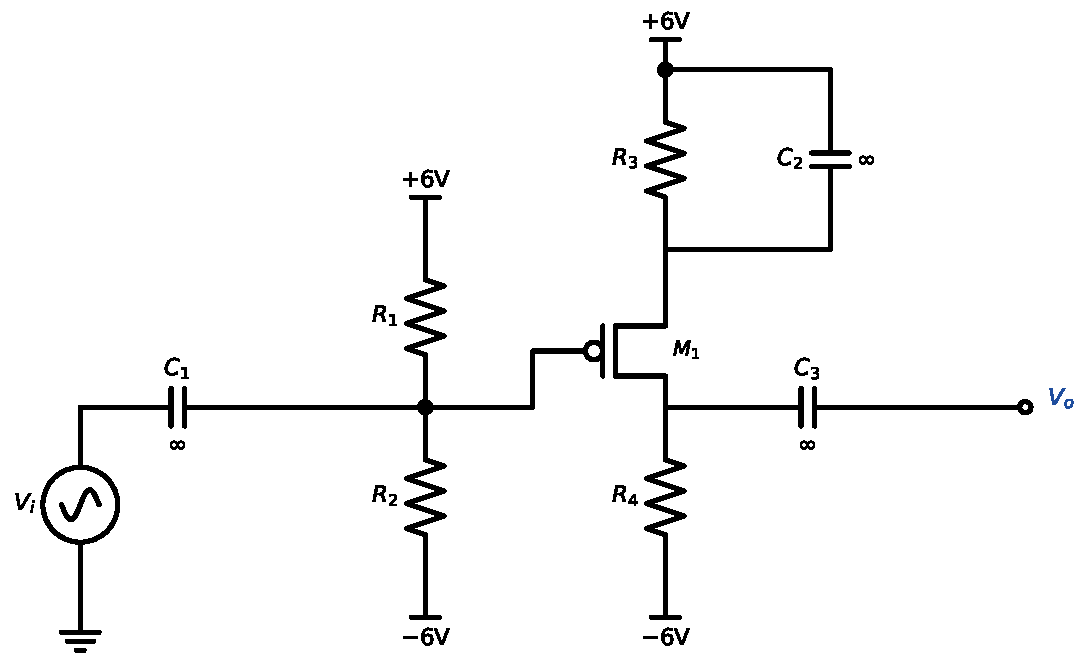
\includegraphics[width=0.9\linewidth,height=6cm,keepaspectratio]{p03_circuit}\end{center}
\solstep{1}{Plan}Follow the procedure of Sample Problem 5: budget the supply voltage around the drain swing; get $V_{ov1}$ from the gain ($|A_v| = g_mR = 2V_R/V_{ov}$), then the resistors; finally the gate divider from the input resistance. Distortion of a common-source stage: $HD_2 \approx \frac{\hat v_{gs}}{4V_{ov}}$ (from $i_D = \frac{k}{2}(V_{ov} + v_{gs})^2$).
\solstep{2}{Design of the stage}Voltage budget of the $V_{DD} + V_{SS} = 12$\,V branch through $R_3$, $M_1$, $R_4$. At its extreme the drain cannot pass the supply on the $R_4$ side: \[V_{R4} \ge \hat V_o = 2\,\mathrm{V}\]$M_1$ must stay active at the other extreme: $V_{R3} + V_{ov1} + \hat V_d + V_{R4} \le 12$, and with $V_{ov1} = 2V_{R4}/|A_{v1}|$ (below): \[V_{R4}\left(1 + \frac{2}{|A_{v1}|}\right) \le 12 - V_{R3} - \hat V_d \Rightarrow V_{R4} \le 7.941\,\mathrm{V}\]$V_{R3} = 1$\,V (its minimum) and $V_{R4} = 6$\,V (given).

Gain of the common-source stage ($R_3$ is bypassed, the follower's gate loads nothing): \[|A_{v1}| = g_{m1}R_4 = k_1V_{ov1}\frac{V_{R4}}{\frac{k_1}{2}V_{ov1}^2} = \frac{2V_{R4}}{V_{ov1}} \Rightarrow V_{ov1} = \frac{2\cdot6}{15} = 0.8\,\mathrm{V}\]$I_{D1} = \frac{k_1}{2}V_{ov1}^2 = 640\,\mu \mathrm{A}$, $R_4 = \frac{V_{R4}}{I_{D1}} = \mathbf{9.37\,\mathrm{k}\Omega}$, $R_3 = \frac{V_{R3}}{I_{D1}} = \mathbf{1.56\,\mathrm{k}\Omega}$.

Gate divider: the resistor on the source side of $M_1$ carries $V_{R1} = V_{R3} + |V_{t1}| + V_{ov1} = 2.6$\,V, the other one $V_{R2} = 12 - 2.6 = 9.4$\,V. Both carry the same current ($I_G = 0$): $R_{1} = 2.6X$, $R_{2} = 9.4X$, and the input resistance is their parallel combination: \[R_1\|R_2 = \frac{2.6\cdot9.4}{12}X \ge 100\,\mathrm{k}\Omega \Rightarrow X = 49.1\,\mathrm{k}\Omega:\quad \mathbf{R_1 = 128\,\mathrm{k}\Omega},\ \mathbf{R_2 = 462\,\mathrm{k}\Omega}\]
\solstep{3}{Check by analysis}DC analysis of the finished circuit (as in sets 5A/5B):\begin{center}\renewcommand{\arraystretch}{1.35}
\begin{tabular}{cccc}
\toprule
 & $I_D$ & $V_{ov}$ & $|V_{DS}|$ \\
\midrule
$M_{1}$ & $640\,\mu \mathrm{A}$ & $0.8$\,V & $5$\,V \\
\bottomrule
\end{tabular}\end{center}
\begin{itemize}[leftmargin=*,itemsep=2pt]
\item $V_{SD1} = V_{S1} - V_{D1} = 5 - 0 = 5\,\mathrm{V}$ $\ge V_{ov1} = 0.8$\,V $\Rightarrow$ $M_{1}$ is active \checkmark
\item Gain (exact small-signal analysis of the finished circuit): $|A_v| = 15$ \checkmark
\item Input resistance $R_1\|R_2 = 100\,\mathrm{k}\Omega \ge 100\,\mathrm{k}\Omega$ \checkmark
\item Output swing before clipping: $M_1$ leaves saturation at $\hat V_o = 4.2$\,V; the drain reaches the supply at $\hat V_o = 6$\,V. The smallest is $4.2$\,V $\ge 2$\,V \checkmark
\item THD $\approx HD_2 = \frac{\hat v_{gs1}}{4V_{ov1}} = \frac{2/15}{4\cdot0.8} = 4.2\,\%$ $\le 5\,\%$ \checkmark
\end{itemize}

\begin{center}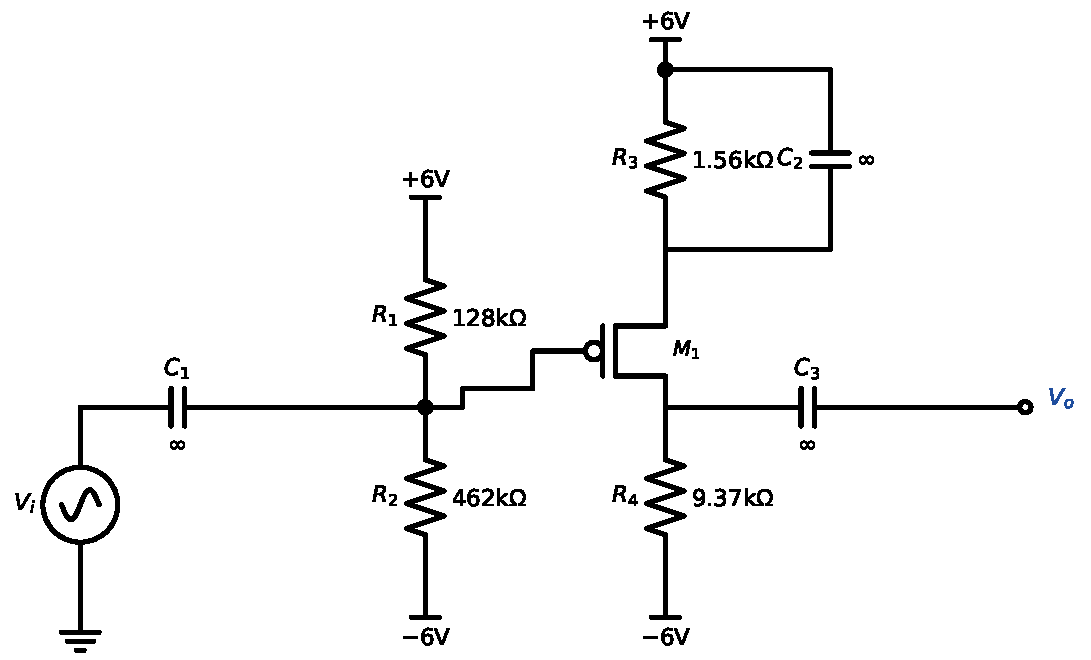
\includegraphics[width=0.85\linewidth,height=6cm,keepaspectratio]{p03_designed}\end{center}

\begin{ansbox}
$R_{1} = 128\,\mathrm{k}\Omega$,\quad $R_{2} = 462\,\mathrm{k}\Omega$,\quad $R_{3} = 1.56\,\mathrm{k}\Omega$,\quad $R_{4} = 9.37\,\mathrm{k}\Omega$
\end{ansbox}

\newpage
\subsection*{Solution 5E.4 \hfill Easy}
\begin{center}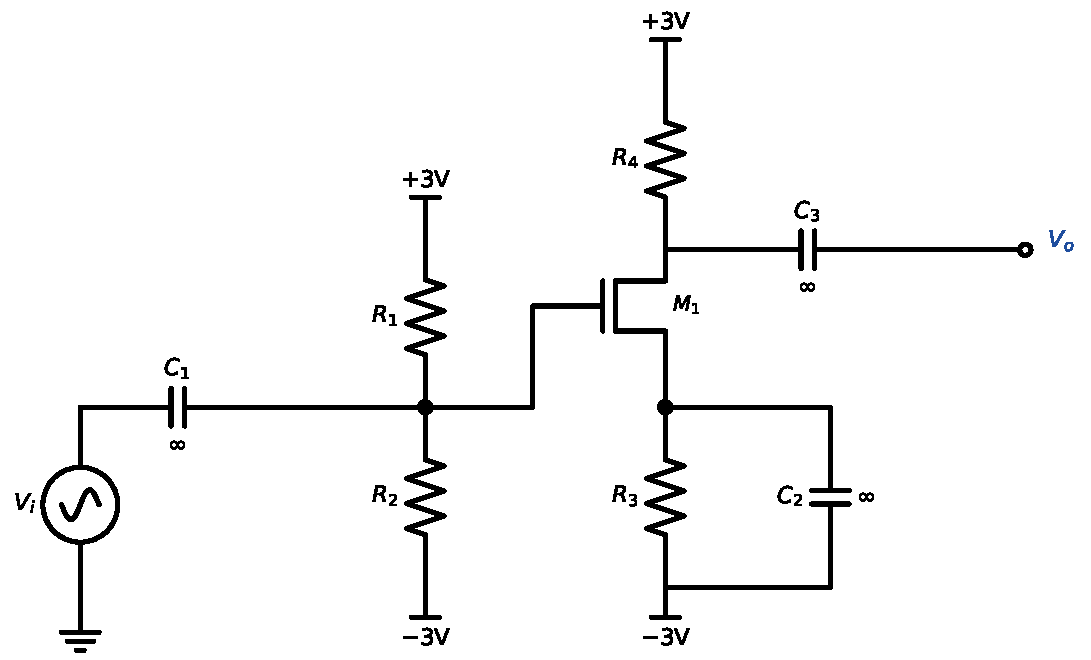
\includegraphics[width=0.9\linewidth,height=6cm,keepaspectratio]{p04_circuit}\end{center}
\solstep{1}{Plan}Follow the procedure of Sample Problem 5: budget the supply voltage around the drain swing; get $V_{ov1}$ from the gain ($|A_v| = g_mR = 2V_R/V_{ov}$), then the resistors; finally the gate divider from the input resistance. Distortion of a common-source stage: $HD_2 \approx \frac{\hat v_{gs}}{4V_{ov}}$ (from $i_D = \frac{k}{2}(V_{ov} + v_{gs})^2$).
\solstep{2}{Design of the stage}Voltage budget of the $V_{DD} + V_{SS} = 6$\,V branch through $R_3$, $M_1$, $R_4$. At its extreme the drain cannot pass the supply on the $R_4$ side: \[V_{R4} \ge \hat V_o = 1\,\mathrm{V}\]$M_1$ must stay active at the other extreme: $V_{R3} + V_{ov1} + \hat V_d + V_{R4} \le 6$, and with $V_{ov1} = 2V_{R4}/|A_{v1}|$ (below): \[V_{R4}\left(1 + \frac{2}{|A_{v1}|}\right) \le 6 - V_{R3} - \hat V_d \Rightarrow V_{R4} \le 3.75\,\mathrm{V}\]$V_{R3} = 0.5$\,V (its minimum) and $V_{R4} = 3$\,V (given).

Gain of the common-source stage ($R_3$ is bypassed, the follower's gate loads nothing): \[|A_{v1}| = g_{m1}R_4 = k_1V_{ov1}\frac{V_{R4}}{\frac{k_1}{2}V_{ov1}^2} = \frac{2V_{R4}}{V_{ov1}} \Rightarrow V_{ov1} = \frac{2\cdot3}{10} = 0.6\,\mathrm{V}\]$I_{D1} = \frac{k_1}{2}V_{ov1}^2 = 90\,\mu \mathrm{A}$, $R_4 = \frac{V_{R4}}{I_{D1}} = \mathbf{33.3\,\mathrm{k}\Omega}$, $R_3 = \frac{V_{R3}}{I_{D1}} = \mathbf{5.56\,\mathrm{k}\Omega}$.

Gate divider: the resistor on the source side of $M_1$ carries $V_{R2} = V_{R3} + |V_{t1}| + V_{ov1} = 1.8$\,V, the other one $V_{R1} = 6 - 1.8 = 4.2$\,V. Both carry the same current ($I_G = 0$): $R_{2} = 1.8X$, $R_{1} = 4.2X$, and the input resistance is their parallel combination: \[R_1\|R_2 = \frac{1.8\cdot4.2}{6}X \ge 50\,\mathrm{k}\Omega \Rightarrow X = 39.7\,\mathrm{k}\Omega:\quad \mathbf{R_1 = 167\,\mathrm{k}\Omega},\ \mathbf{R_2 = 71.4\,\mathrm{k}\Omega}\]
\solstep{3}{Check by analysis}DC analysis of the finished circuit (as in sets 5A/5B):\begin{center}\renewcommand{\arraystretch}{1.35}
\begin{tabular}{cccc}
\toprule
 & $I_D$ & $V_{ov}$ & $|V_{DS}|$ \\
\midrule
$M_{1}$ & $90\,\mu \mathrm{A}$ & $0.6$\,V & $2.5$\,V \\
\bottomrule
\end{tabular}\end{center}
\begin{itemize}[leftmargin=*,itemsep=2pt]
\item $V_{DS1} = V_{D1} - V_{S1} = 1.355\times 10^{-15} - (-2.5) = 2.5\,\mathrm{V}$ $\ge V_{ov1} = 0.6$\,V $\Rightarrow$ $M_{1}$ is active \checkmark
\item Gain (exact small-signal analysis of the finished circuit): $|A_v| = 10$ \checkmark
\item Input resistance $R_1\|R_2 = 50\,\mathrm{k}\Omega \ge 50\,\mathrm{k}\Omega$ \checkmark
\item Output swing before clipping: $M_1$ leaves saturation at $\hat V_o = 1.9$\,V; the drain reaches the supply at $\hat V_o = 3$\,V. The smallest is $1.9$\,V $\ge 1$\,V \checkmark
\item THD $\approx HD_2 = \frac{\hat v_{gs1}}{4V_{ov1}} = \frac{1/10}{4\cdot0.6} = 4.2\,\%$ $\le 5\,\%$ \checkmark
\end{itemize}

\begin{center}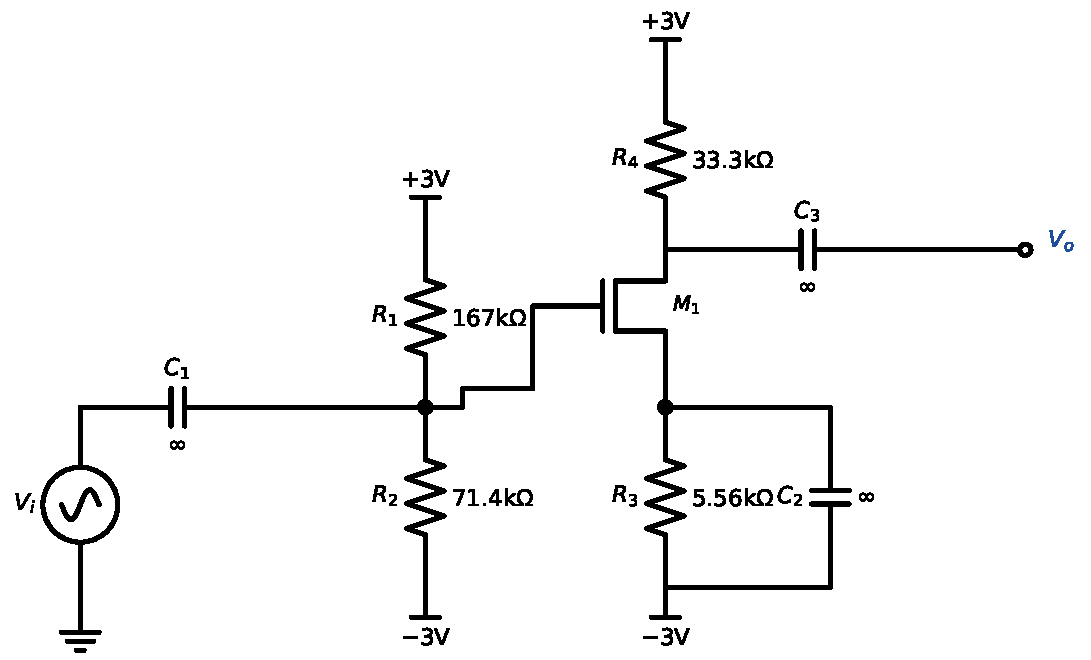
\includegraphics[width=0.85\linewidth,height=6cm,keepaspectratio]{p04_designed}\end{center}

\begin{ansbox}
$R_{1} = 167\,\mathrm{k}\Omega$,\quad $R_{2} = 71.4\,\mathrm{k}\Omega$,\quad $R_{3} = 5.56\,\mathrm{k}\Omega$,\quad $R_{4} = 33.3\,\mathrm{k}\Omega$
\end{ansbox}

\newpage
\subsection*{Solution 5E.5 \hfill Easy}
\begin{center}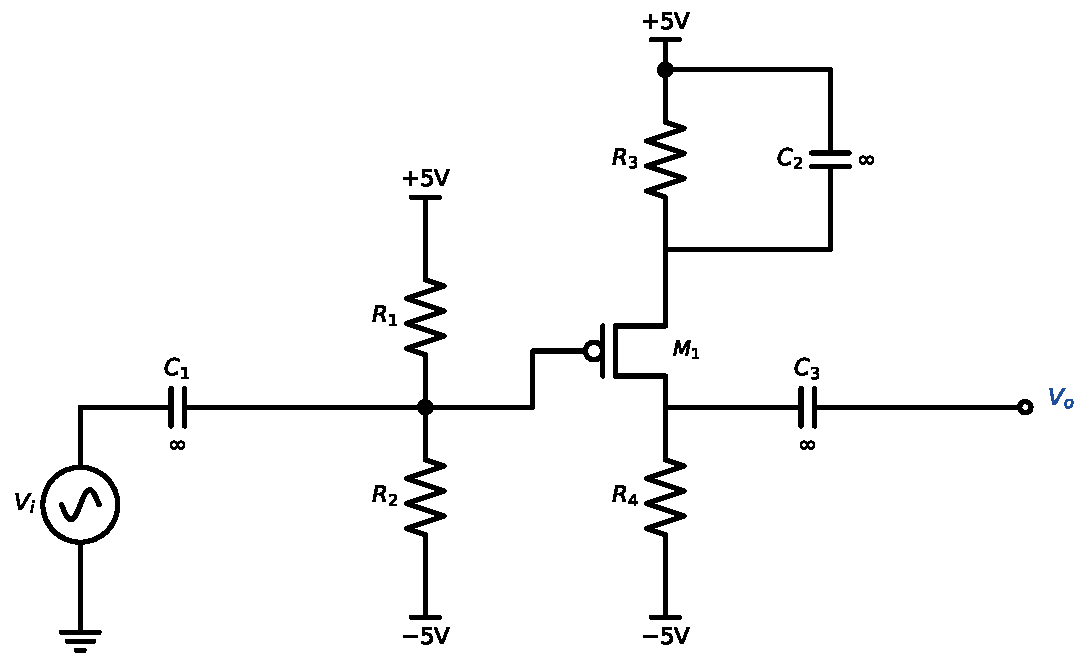
\includegraphics[width=0.9\linewidth,height=6cm,keepaspectratio]{p05_circuit}\end{center}
\solstep{1}{Plan}Follow the procedure of Sample Problem 5: budget the supply voltage around the drain swing; get $V_{ov1}$ from the gain ($|A_v| = g_mR = 2V_R/V_{ov}$), then the resistors; finally the gate divider from the input resistance. Distortion of a common-source stage: $HD_2 \approx \frac{\hat v_{gs}}{4V_{ov}}$ (from $i_D = \frac{k}{2}(V_{ov} + v_{gs})^2$).
\solstep{2}{Design of the stage}Voltage budget of the $V_{DD} + V_{SS} = 10$\,V branch through $R_3$, $M_1$, $R_4$. At its extreme the drain cannot pass the supply on the $R_4$ side: \[V_{R4} \ge \hat V_o = 1\,\mathrm{V}\]$M_1$ must stay active at the other extreme: $V_{R3} + V_{ov1} + \hat V_d + V_{R4} \le 10$, and with $V_{ov1} = 2V_{R4}/|A_{v1}|$ (below): \[V_{R4}\left(1 + \frac{2}{|A_{v1}|}\right) \le 10 - V_{R3} - \hat V_d \Rightarrow V_{R4} \le 8.095\,\mathrm{V}\]$V_{R3} = 0.5$\,V (its minimum) and $V_{R4} = 6$\,V (given).

Gain of the common-source stage ($R_3$ is bypassed, the follower's gate loads nothing): \[|A_{v1}| = g_{m1}R_4 = k_1V_{ov1}\frac{V_{R4}}{\frac{k_1}{2}V_{ov1}^2} = \frac{2V_{R4}}{V_{ov1}} \Rightarrow V_{ov1} = \frac{2\cdot6}{40} = 0.3\,\mathrm{V}\]$I_{D1} = \frac{k_1}{2}V_{ov1}^2 = 45\,\mu \mathrm{A}$, $R_4 = \frac{V_{R4}}{I_{D1}} = \mathbf{133\,\mathrm{k}\Omega}$, $R_3 = \frac{V_{R3}}{I_{D1}} = \mathbf{11.1\,\mathrm{k}\Omega}$.

Gate divider: the resistor on the source side of $M_1$ carries $V_{R1} = V_{R3} + |V_{t1}| + V_{ov1} = 1.8$\,V, the other one $V_{R2} = 10 - 1.8 = 8.2$\,V. Both carry the same current ($I_G = 0$): $R_{1} = 1.8X$, $R_{2} = 8.2X$, and the input resistance is their parallel combination: \[R_1\|R_2 = \frac{1.8\cdot8.2}{10}X \ge 1\,\mathrm{M}\Omega \Rightarrow X = 678\,\mathrm{k}\Omega:\quad \mathbf{R_1 = 1.22\,\mathrm{M}\Omega},\ \mathbf{R_2 = 5.56\,\mathrm{M}\Omega}\]
\solstep{3}{Check by analysis}DC analysis of the finished circuit (as in sets 5A/5B):\begin{center}\renewcommand{\arraystretch}{1.35}
\begin{tabular}{cccc}
\toprule
 & $I_D$ & $V_{ov}$ & $|V_{DS}|$ \\
\midrule
$M_{1}$ & $45\,\mu \mathrm{A}$ & $0.3$\,V & $3.5$\,V \\
\bottomrule
\end{tabular}\end{center}
\begin{itemize}[leftmargin=*,itemsep=2pt]
\item $V_{SD1} = V_{S1} - V_{D1} = 4.5 - 1 = 3.5\,\mathrm{V}$ $\ge V_{ov1} = 0.3$\,V $\Rightarrow$ $M_{1}$ is active \checkmark
\item Gain (exact small-signal analysis of the finished circuit): $|A_v| = 40$ \checkmark
\item Input resistance $R_1\|R_2 = 1\,\mathrm{M}\Omega \ge 1\,\mathrm{M}\Omega$ \checkmark
\item Output swing before clipping: $M_1$ leaves saturation at $\hat V_o = 3.2$\,V; the drain reaches the supply at $\hat V_o = 6$\,V. The smallest is $3.2$\,V $\ge 1$\,V \checkmark
\item THD $\approx HD_2 = \frac{\hat v_{gs1}}{4V_{ov1}} = \frac{1/40}{4\cdot0.3} = 2.1\,\%$ $\le 3\,\%$ \checkmark
\end{itemize}

\begin{center}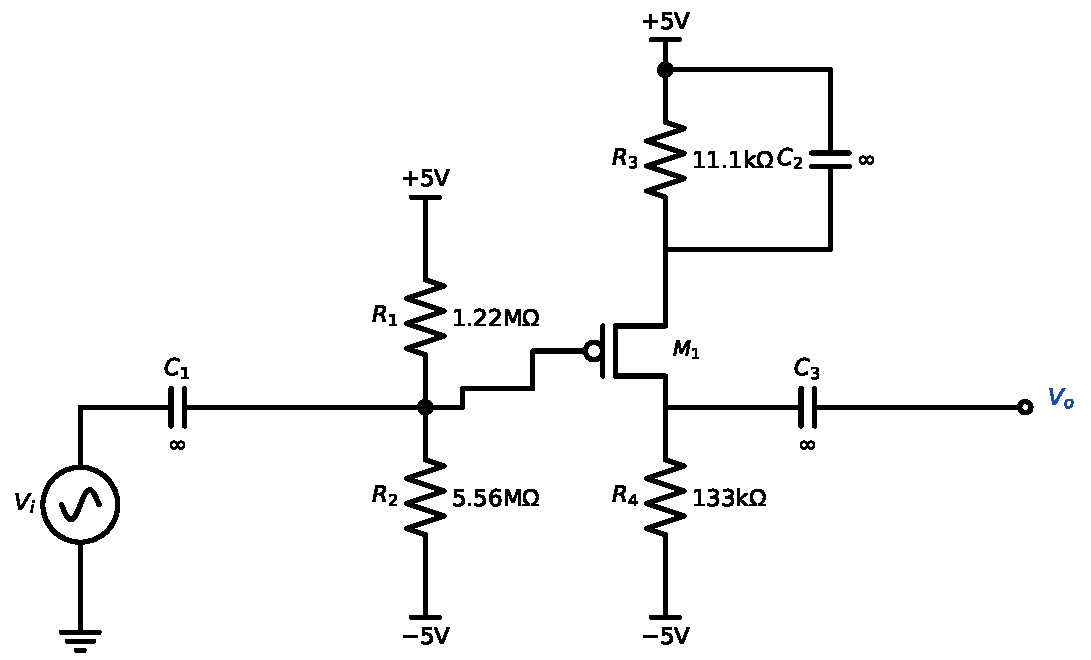
\includegraphics[width=0.85\linewidth,height=6cm,keepaspectratio]{p05_designed}\end{center}

\begin{ansbox}
$R_{1} = 1.22\,\mathrm{M}\Omega$,\quad $R_{2} = 5.56\,\mathrm{M}\Omega$,\quad $R_{3} = 11.1\,\mathrm{k}\Omega$,\quad $R_{4} = 133\,\mathrm{k}\Omega$
\end{ansbox}

\newpage
\subsection*{Solution 5E.6 \hfill Easy}
\begin{center}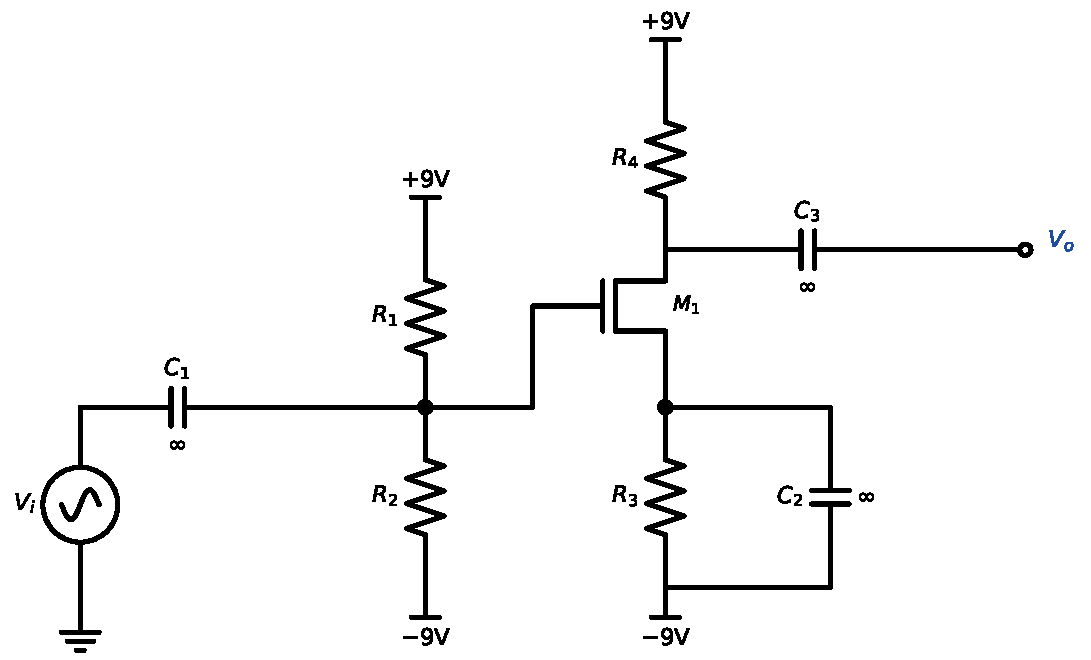
\includegraphics[width=0.9\linewidth,height=6cm,keepaspectratio]{p06_circuit}\end{center}
\solstep{1}{Plan}Follow the procedure of Sample Problem 5: budget the supply voltage around the drain swing; get $V_{ov1}$ from the gain ($|A_v| = g_mR = 2V_R/V_{ov}$), then the resistors; finally the gate divider from the input resistance. Distortion of a common-source stage: $HD_2 \approx \frac{\hat v_{gs}}{4V_{ov}}$ (from $i_D = \frac{k}{2}(V_{ov} + v_{gs})^2$).
\solstep{2}{Design of the stage}Voltage budget of the $V_{DD} + V_{SS} = 18$\,V branch through $R_3$, $M_1$, $R_4$. At its extreme the drain cannot pass the supply on the $R_4$ side: \[V_{R4} \ge \hat V_o = 3\,\mathrm{V}\]$M_1$ must stay active at the other extreme: $V_{R3} + V_{ov1} + \hat V_d + V_{R4} \le 18$, and with $V_{ov1} = 2V_{R4}/|A_{v1}|$ (below): \[V_{R4}\left(1 + \frac{2}{|A_{v1}|}\right) \le 18 - V_{R3} - \hat V_d \Rightarrow V_{R4} \le 13.12\,\mathrm{V}\]$V_{R3} = 1$\,V (its minimum) and $V_{R4} = 9$\,V (given).

Gain of the common-source stage ($R_3$ is bypassed, the follower's gate loads nothing): \[|A_{v1}| = g_{m1}R_4 = k_1V_{ov1}\frac{V_{R4}}{\frac{k_1}{2}V_{ov1}^2} = \frac{2V_{R4}}{V_{ov1}} \Rightarrow V_{ov1} = \frac{2\cdot9}{30} = 0.6\,\mathrm{V}\]$I_{D1} = \frac{k_1}{2}V_{ov1}^2 = 180\,\mu \mathrm{A}$, $R_4 = \frac{V_{R4}}{I_{D1}} = \mathbf{50\,\mathrm{k}\Omega}$, $R_3 = \frac{V_{R3}}{I_{D1}} = \mathbf{5.56\,\mathrm{k}\Omega}$.

Gate divider: the resistor on the source side of $M_1$ carries $V_{R2} = V_{R3} + |V_{t1}| + V_{ov1} = 2.6$\,V, the other one $V_{R1} = 18 - 2.6 = 15.4$\,V. Both carry the same current ($I_G = 0$): $R_{2} = 2.6X$, $R_{1} = 15.4X$, and the input resistance is their parallel combination: \[R_1\|R_2 = \frac{2.6\cdot15.4}{18}X \ge 500\,\mathrm{k}\Omega \Rightarrow X = 225\,\mathrm{k}\Omega:\quad \mathbf{R_1 = 3.46\,\mathrm{M}\Omega},\ \mathbf{R_2 = 584\,\mathrm{k}\Omega}\]
\solstep{3}{Check by analysis}DC analysis of the finished circuit (as in sets 5A/5B):\begin{center}\renewcommand{\arraystretch}{1.35}
\begin{tabular}{cccc}
\toprule
 & $I_D$ & $V_{ov}$ & $|V_{DS}|$ \\
\midrule
$M_{1}$ & $180\,\mu \mathrm{A}$ & $0.6$\,V & $8$\,V \\
\bottomrule
\end{tabular}\end{center}
\begin{itemize}[leftmargin=*,itemsep=2pt]
\item $V_{DS1} = V_{D1} - V_{S1} = -4.066\times 10^{-15} - (-8) = 8\,\mathrm{V}$ $\ge V_{ov1} = 0.6$\,V $\Rightarrow$ $M_{1}$ is active \checkmark
\item Gain (exact small-signal analysis of the finished circuit): $|A_v| = 30$ \checkmark
\item Input resistance $R_1\|R_2 = 500\,\mathrm{k}\Omega \ge 500\,\mathrm{k}\Omega$ \checkmark
\item Output swing before clipping: $M_1$ leaves saturation at $\hat V_o = 7.4$\,V; the drain reaches the supply at $\hat V_o = 9$\,V. The smallest is $7.4$\,V $\ge 3$\,V \checkmark
\item THD $\approx HD_2 = \frac{\hat v_{gs1}}{4V_{ov1}} = \frac{3/30}{4\cdot0.6} = 4.2\,\%$ $\le 5\,\%$ \checkmark
\end{itemize}

\begin{center}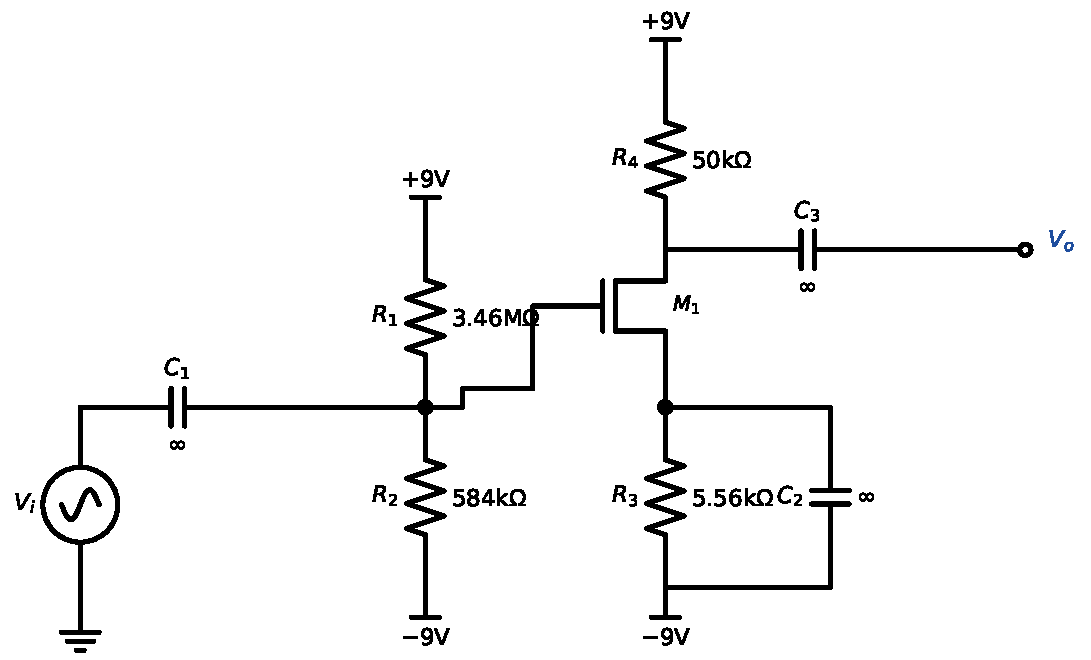
\includegraphics[width=0.85\linewidth,height=6cm,keepaspectratio]{p06_designed}\end{center}

\begin{ansbox}
$R_{1} = 3.46\,\mathrm{M}\Omega$,\quad $R_{2} = 584\,\mathrm{k}\Omega$,\quad $R_{3} = 5.56\,\mathrm{k}\Omega$,\quad $R_{4} = 50\,\mathrm{k}\Omega$
\end{ansbox}

\newpage
\subsection*{Solution 5E.7 \hfill Medium}
\begin{center}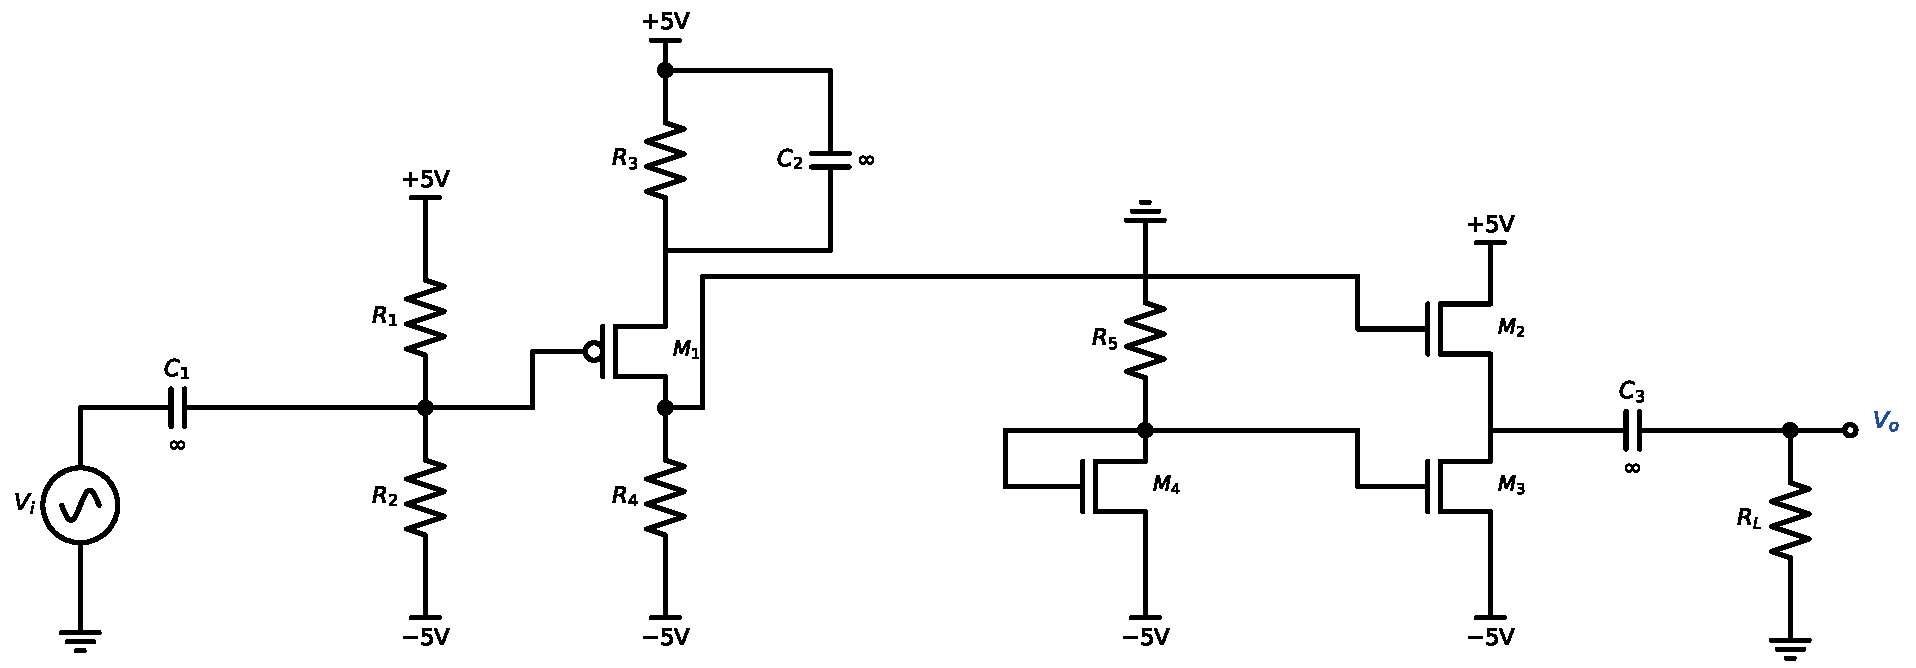
\includegraphics[width=0.9\linewidth,height=6cm,keepaspectratio]{p07_circuit}\end{center}
\solstep{1}{Plan}Follow the procedure of Sample Problem 5: size the output current sink for the load current, then the follower; budget the supply voltage around the drain swing; get $V_{ov1}$ from the gain ($|A_v| = g_mR = 2V_R/V_{ov}$), then the resistors; finally the gate divider from the input resistance. Distortion of a common-source stage: $HD_2 \approx \frac{\hat v_{gs}}{4V_{ov}}$ (from $i_D = \frac{k}{2}(V_{ov} + v_{gs})^2$).
\solstep{2}{Output stage: sink, reference and follower}The sink $M_3$ must deliver the whole peak load current: $I_{D3} \ge \frac{\hat V_o}{R_L} = \frac{1}{200\,\Omega} = 5\,\mathrm{m}\mathrm{A}$; use $I_{D3} = 10\,\mathrm{m}\mathrm{A}$ (given). Then $\frac{k_3}{2}V_{ov3}^2 = I_{D3} \Rightarrow V_{ov3} = \sqrt{\frac{2\cdot10\,\mathrm{m}\mathrm{A}}{50\,\mathrm{m}\mathrm{A/V^2}}} = 0.6325$\,V.

$M_4$ is identical to $M_3$ and has the same $V_{GS}$, so $I_{D4} = I_{D3}$ and $V_{ov4} = V_{ov3}$.

\[R_5 = \frac{5 - |V_{t}| - V_{ov4}}{I_{D4}} = \frac{5 - 2 - 0.6325}{10\,\mathrm{m}\mathrm{A}} = \mathbf{237\,\Omega}\]

The follower $M_2$ carries the same current, $I_{D2} = I_{D3}$, so $V_{ov2} = 0.6325$\,V, $g_{m2} = k_2V_{ov2} = 31.6\,\mathrm{m}\mathrm{A/V}$, $1/g_{m2} = 31.6\,\Omega$ and (the sink $M_3$ is a current source, $Z = \infty$) \[A_{v2} = \frac{R_L}{1/g_{m2} + R_L} = \frac{200\,\Omega}{31.6\,\Omega + 200\,\Omega} = 0.8635\]So the drain of $M_1$ must swing $\hat V_d = \hat V_o/A_{v2} = 1.158$\,V and $|A_{v1}| = |A_v|/A_{v2} = 23.16$.
\solstep{3}{Common-source stage}Voltage budget of the $V_{DD} + V_{SS} = 10$\,V branch through $R_3$, $M_1$, $R_4$. At the lowest drain voltage of $M_1$ the follower and the sink must both stay active (the drain of $M_1$ sits one $|V_{GS2}|$ away from the output, which needs $V_{ov3}$ of room above the rail): \[V_{R4} \ge V_{ov3} + V_{ov2} + |V_{t2}| + \hat V_d = 0.632 + 0.632 + 2 + 1.16 = 4.423\,\mathrm{V}\]$M_1$ must stay active at the other extreme: $V_{R3} + V_{ov1} + \hat V_d + V_{R4} \le 10$, and with $V_{ov1} = 2V_{R4}/|A_{v1}|$ (below): \[V_{R4}\left(1 + \frac{2}{|A_{v1}|}\right) \le 10 - V_{R3} - \hat V_d \Rightarrow V_{R4} \le 7.679\,\mathrm{V}\]$V_{R3} = 0.5$\,V (its minimum) and $V_{R4} = 4.5$\,V (the next multiple of $0.5$\,V above the lower bound).

Gain of the common-source stage ($R_3$ is bypassed, the follower's gate loads nothing): \[|A_{v1}| = g_{m1}R_4 = k_1V_{ov1}\frac{V_{R4}}{\frac{k_1}{2}V_{ov1}^2} = \frac{2V_{R4}}{V_{ov1}} \Rightarrow V_{ov1} = \frac{2\cdot4.5}{23.16} = 0.3886\,\mathrm{V}\]$I_{D1} = \frac{k_1}{2}V_{ov1}^2 = 75.5\,\mu \mathrm{A}$, $R_4 = \frac{V_{R4}}{I_{D1}} = \mathbf{59.6\,\mathrm{k}\Omega}$, $R_3 = \frac{V_{R3}}{I_{D1}} = \mathbf{6.62\,\mathrm{k}\Omega}$.

Gate divider: the resistor on the source side of $M_1$ carries $V_{R1} = V_{R3} + |V_{t1}| + V_{ov1} = 1.889$\,V, the other one $V_{R2} = 10 - 1.889 = 8.111$\,V. Both carry the same current ($I_G = 0$): $R_{1} = 1.889X$, $R_{2} = 8.111X$, and the input resistance is their parallel combination: \[R_1\|R_2 = \frac{1.889\cdot8.111}{10}X \ge 100\,\mathrm{k}\Omega \Rightarrow X = 65.3\,\mathrm{k}\Omega:\quad \mathbf{R_1 = 123\,\mathrm{k}\Omega},\ \mathbf{R_2 = 530\,\mathrm{k}\Omega}\]
\solstep{4}{Check by analysis}DC analysis of the finished circuit (as in sets 5A/5B):\begin{center}\renewcommand{\arraystretch}{1.35}
\begin{tabular}{cccc}
\toprule
 & $I_D$ & $V_{ov}$ & $|V_{DS}|$ \\
\midrule
$M_{1}$ & $75.5\,\mu \mathrm{A}$ & $0.389$\,V & $5$\,V \\
$M_{4}$ & $10\,\mathrm{m}\mathrm{A}$ & $0.632$\,V & $2.632$\,V \\
$M_{2}$ & $10\,\mathrm{m}\mathrm{A}$ & $0.632$\,V & $8.132$\,V \\
$M_{3}$ & $10\,\mathrm{m}\mathrm{A}$ & $0.632$\,V & $1.868$\,V \\
\bottomrule
\end{tabular}\end{center}
\begin{itemize}[leftmargin=*,itemsep=2pt]
\item $V_{SD1} = V_{S1} - V_{D1} = 4.5 - (-0.5) = 5\,\mathrm{V}$ $\ge V_{ov1} = 0.389$\,V $\Rightarrow$ $M_{1}$ is active \checkmark
\item $M_{4}$ is diode-connected: $V_{DS4} = V_{GS4} > V_{ov4}$, always active \checkmark
\item $V_{DS2} = 5 - V_{S2} = 5 - (-3.132) = 8.13\,\mathrm{V}$ $\ge V_{ov2} = 0.632$\,V $\Rightarrow$ $M_{2}$ is active \checkmark
\item $V_{DS3} = V_{S2} - (-5) = -3.132 - (-5) = 1.87\,\mathrm{V}$ $\ge V_{ov3} = 0.632$\,V $\Rightarrow$ $M_{3}$ is active \checkmark
\item Gain (exact small-signal analysis of the finished circuit): $|A_v| = 20$ \checkmark
\item Input resistance $R_1\|R_2 = 100\,\mathrm{k}\Omega \ge 100\,\mathrm{k}\Omega$ \checkmark
\item Output swing before clipping: $M_1$ leaves saturation at $\hat V_o = 3.98$\,V; $M_3$ leaves saturation at $\hat V_o = 1.24$\,V; $M_2$ leaves saturation at $\hat V_o = 7.5$\,V; $M_3$ cannot sink more current (current clipping) at $\hat V_o = 2$\,V. The smallest is $1.24$\,V $\ge 1$\,V \checkmark
\item THD $\approx HD_2 = \frac{\hat v_{gs1}}{4V_{ov1}} = \frac{1/20}{4\cdot0.389} = 3.2\,\%$ $\le 10\,\%$ \checkmark
\end{itemize}

\begin{center}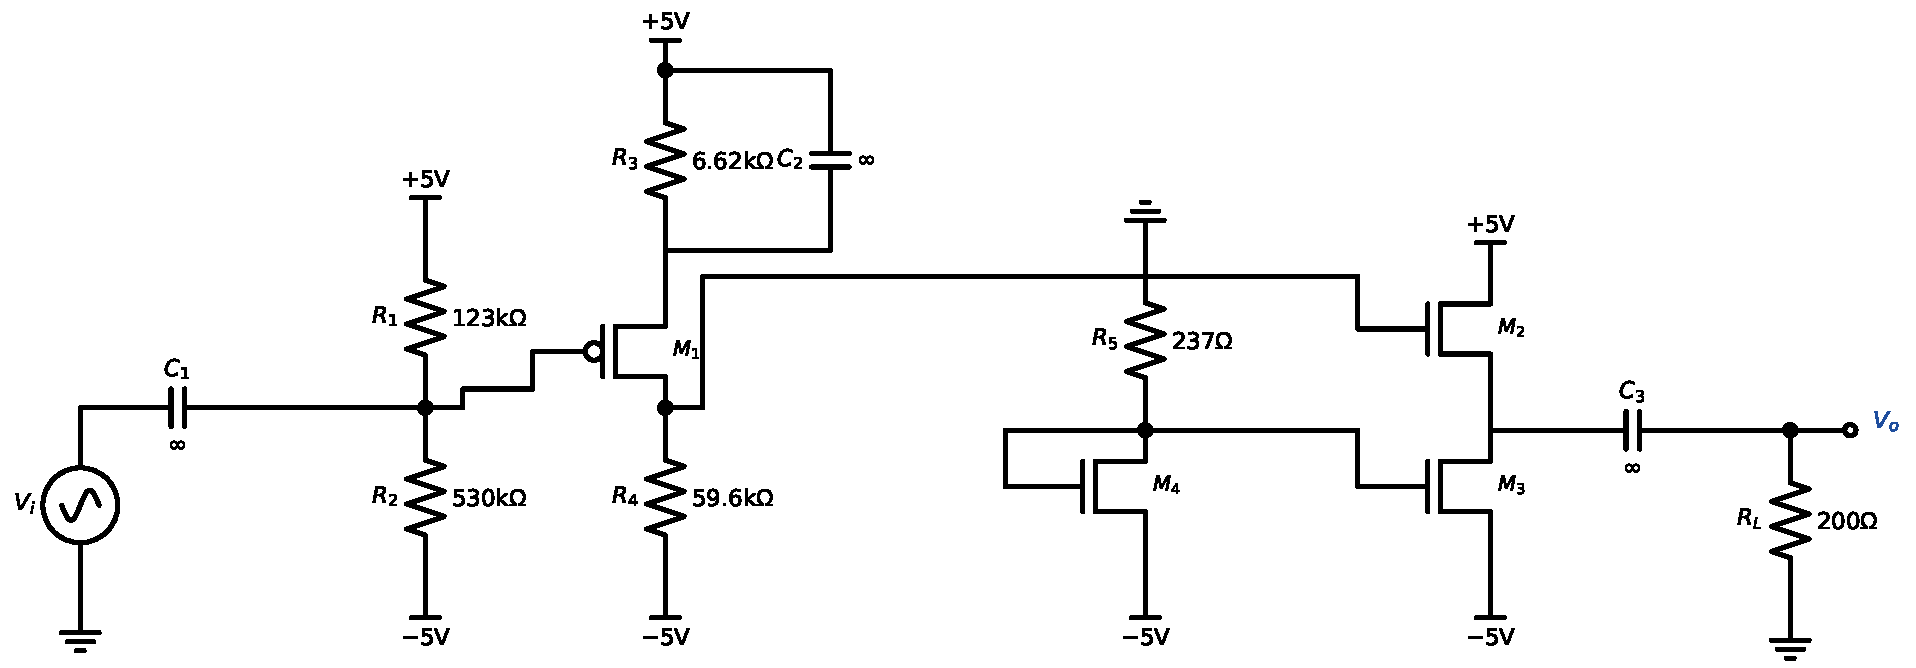
\includegraphics[width=0.85\linewidth,height=6cm,keepaspectratio]{p07_designed}\end{center}

\begin{ansbox}
$R_{1} = 123\,\mathrm{k}\Omega$,\quad $R_{2} = 530\,\mathrm{k}\Omega$,\quad $R_{3} = 6.62\,\mathrm{k}\Omega$,\quad $R_{4} = 59.6\,\mathrm{k}\Omega$,\quad $R_{5} = 237\,\Omega$
\end{ansbox}

\newpage
\subsection*{Solution 5E.8 \hfill Medium}
\begin{center}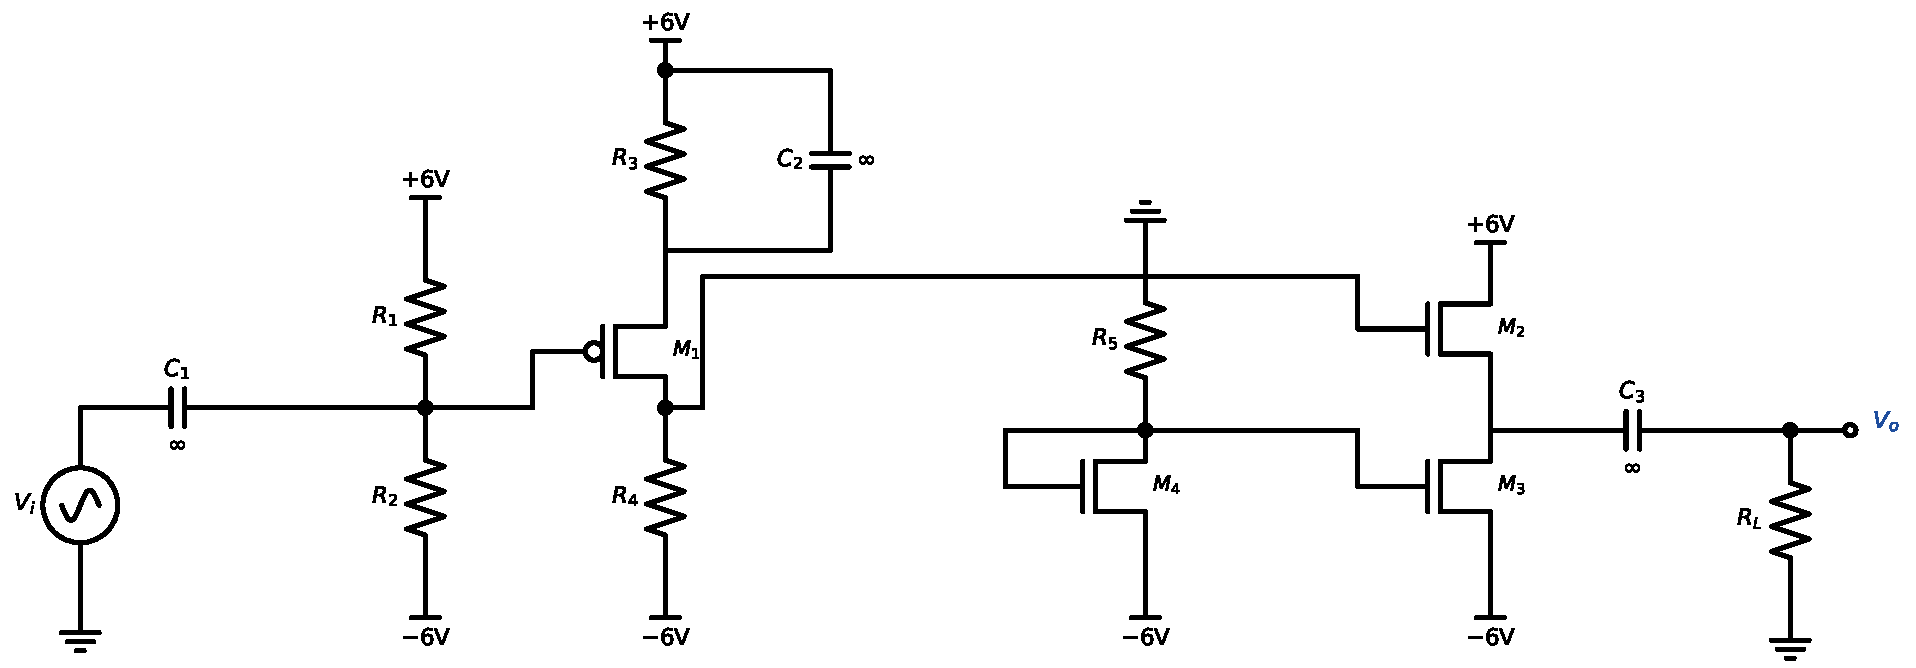
\includegraphics[width=0.9\linewidth,height=6cm,keepaspectratio]{p08_circuit}\end{center}
\solstep{1}{Plan}Follow the procedure of Sample Problem 5: size the output current sink for the load current, then the follower; budget the supply voltage around the drain swing; get $V_{ov1}$ from the gain ($|A_v| = g_mR = 2V_R/V_{ov}$), then the resistors; finally the gate divider from the input resistance. Distortion of a common-source stage: $HD_2 \approx \frac{\hat v_{gs}}{4V_{ov}}$ (from $i_D = \frac{k}{2}(V_{ov} + v_{gs})^2$).
\solstep{2}{Output stage: sink, reference and follower}The sink $M_3$ must deliver the whole peak load current: $I_{D3} \ge \frac{\hat V_o}{R_L} = \frac{2}{500\,\Omega} = 4\,\mathrm{m}\mathrm{A}$; use $I_{D3} = 5\,\mathrm{m}\mathrm{A}$ (given). Then $\frac{k_3}{2}V_{ov3}^2 = I_{D3} \Rightarrow V_{ov3} = \sqrt{\frac{2\cdot5\,\mathrm{m}\mathrm{A}}{50\,\mathrm{m}\mathrm{A/V^2}}} = 0.4472$\,V.

$M_4$ is identical to $M_3$ and has the same $V_{GS}$, so $I_{D4} = I_{D3}$ and $V_{ov4} = V_{ov3}$.

\[R_5 = \frac{6 - |V_{t}| - V_{ov4}}{I_{D4}} = \frac{6 - 2 - 0.4472}{5\,\mathrm{m}\mathrm{A}} = \mathbf{711\,\Omega}\]

The follower $M_2$ carries the same current, $I_{D2} = I_{D3}$, so $V_{ov2} = 0.4472$\,V, $g_{m2} = k_2V_{ov2} = 22.4\,\mathrm{m}\mathrm{A/V}$, $1/g_{m2} = 44.7\,\Omega$ and (the sink $M_3$ is a current source, $Z = \infty$) \[A_{v2} = \frac{R_L}{1/g_{m2} + R_L} = \frac{500\,\Omega}{44.7\,\Omega + 500\,\Omega} = 0.9179\]So the drain of $M_1$ must swing $\hat V_d = \hat V_o/A_{v2} = 2.179$\,V and $|A_{v1}| = |A_v|/A_{v2} = 32.68$.
\solstep{3}{Common-source stage}Voltage budget of the $V_{DD} + V_{SS} = 12$\,V branch through $R_3$, $M_1$, $R_4$. At the lowest drain voltage of $M_1$ the follower and the sink must both stay active (the drain of $M_1$ sits one $|V_{GS2}|$ away from the output, which needs $V_{ov3}$ of room above the rail): \[V_{R4} \ge V_{ov3} + V_{ov2} + |V_{t2}| + \hat V_d = 0.447 + 0.447 + 2 + 2.18 = 5.073\,\mathrm{V}\]$M_1$ must stay active at the other extreme: $V_{R3} + V_{ov1} + \hat V_d + V_{R4} \le 12$, and with $V_{ov1} = 2V_{R4}/|A_{v1}|$ (below): \[V_{R4}\left(1 + \frac{2}{|A_{v1}|}\right) \le 12 - V_{R3} - \hat V_d \Rightarrow V_{R4} \le 8.784\,\mathrm{V}\]$V_{R3} = 0.5$\,V (its minimum) and $V_{R4} = 5.5$\,V (the next multiple of $0.5$\,V above the lower bound).

Gain of the common-source stage ($R_3$ is bypassed, the follower's gate loads nothing): \[|A_{v1}| = g_{m1}R_4 = k_1V_{ov1}\frac{V_{R4}}{\frac{k_1}{2}V_{ov1}^2} = \frac{2V_{R4}}{V_{ov1}} \Rightarrow V_{ov1} = \frac{2\cdot5.5}{32.68} = 0.3366\,\mathrm{V}\]$I_{D1} = \frac{k_1}{2}V_{ov1}^2 = 56.6\,\mu \mathrm{A}$, $R_4 = \frac{V_{R4}}{I_{D1}} = \mathbf{97.1\,\mathrm{k}\Omega}$, $R_3 = \frac{V_{R3}}{I_{D1}} = \mathbf{8.83\,\mathrm{k}\Omega}$.

Gate divider: the resistor on the source side of $M_1$ carries $V_{R1} = V_{R3} + |V_{t1}| + V_{ov1} = 1.837$\,V, the other one $V_{R2} = 12 - 1.837 = 10.16$\,V. Both carry the same current ($I_G = 0$): $R_{1} = 1.837X$, $R_{2} = 10.16X$, and the input resistance is their parallel combination: \[R_1\|R_2 = \frac{1.837\cdot10.16}{12}X \ge 200\,\mathrm{k}\Omega \Rightarrow X = 129\,\mathrm{k}\Omega:\quad \mathbf{R_1 = 236\,\mathrm{k}\Omega},\ \mathbf{R_2 = 1.31\,\mathrm{M}\Omega}\]
\solstep{4}{Check by analysis}DC analysis of the finished circuit (as in sets 5A/5B):\begin{center}\renewcommand{\arraystretch}{1.35}
\begin{tabular}{cccc}
\toprule
 & $I_D$ & $V_{ov}$ & $|V_{DS}|$ \\
\midrule
$M_{1}$ & $56.6\,\mu \mathrm{A}$ & $0.337$\,V & $6$\,V \\
$M_{4}$ & $5\,\mathrm{m}\mathrm{A}$ & $0.447$\,V & $2.447$\,V \\
$M_{2}$ & $5\,\mathrm{m}\mathrm{A}$ & $0.447$\,V & $8.947$\,V \\
$M_{3}$ & $5\,\mathrm{m}\mathrm{A}$ & $0.447$\,V & $3.053$\,V \\
\bottomrule
\end{tabular}\end{center}
\begin{itemize}[leftmargin=*,itemsep=2pt]
\item $V_{SD1} = V_{S1} - V_{D1} = 5.5 - (-0.5) = 6\,\mathrm{V}$ $\ge V_{ov1} = 0.337$\,V $\Rightarrow$ $M_{1}$ is active \checkmark
\item $M_{4}$ is diode-connected: $V_{DS4} = V_{GS4} > V_{ov4}$, always active \checkmark
\item $V_{DS2} = 6 - V_{S2} = 6 - (-2.947) = 8.95\,\mathrm{V}$ $\ge V_{ov2} = 0.447$\,V $\Rightarrow$ $M_{2}$ is active \checkmark
\item $V_{DS3} = V_{S2} - (-6) = -2.947 - (-6) = 3.05\,\mathrm{V}$ $\ge V_{ov3} = 0.447$\,V $\Rightarrow$ $M_{3}$ is active \checkmark
\item Gain (exact small-signal analysis of the finished circuit): $|A_v| = 30$ \checkmark
\item Input resistance $R_1\|R_2 = 200\,\mathrm{k}\Omega \ge 200\,\mathrm{k}\Omega$ \checkmark
\item Output swing before clipping: $M_1$ leaves saturation at $\hat V_o = 5.2$\,V; $M_3$ leaves saturation at $\hat V_o = 2.61$\,V; $M_2$ leaves saturation at $\hat V_o = 8.5$\,V; $M_3$ cannot sink more current (current clipping) at $\hat V_o = 2.5$\,V. The smallest is $2.5$\,V $\ge 2$\,V \checkmark
\item THD $\approx HD_2 = \frac{\hat v_{gs1}}{4V_{ov1}} = \frac{2/30}{4\cdot0.337} = 5\,\%$ $\le 10\,\%$ \checkmark
\end{itemize}

\begin{center}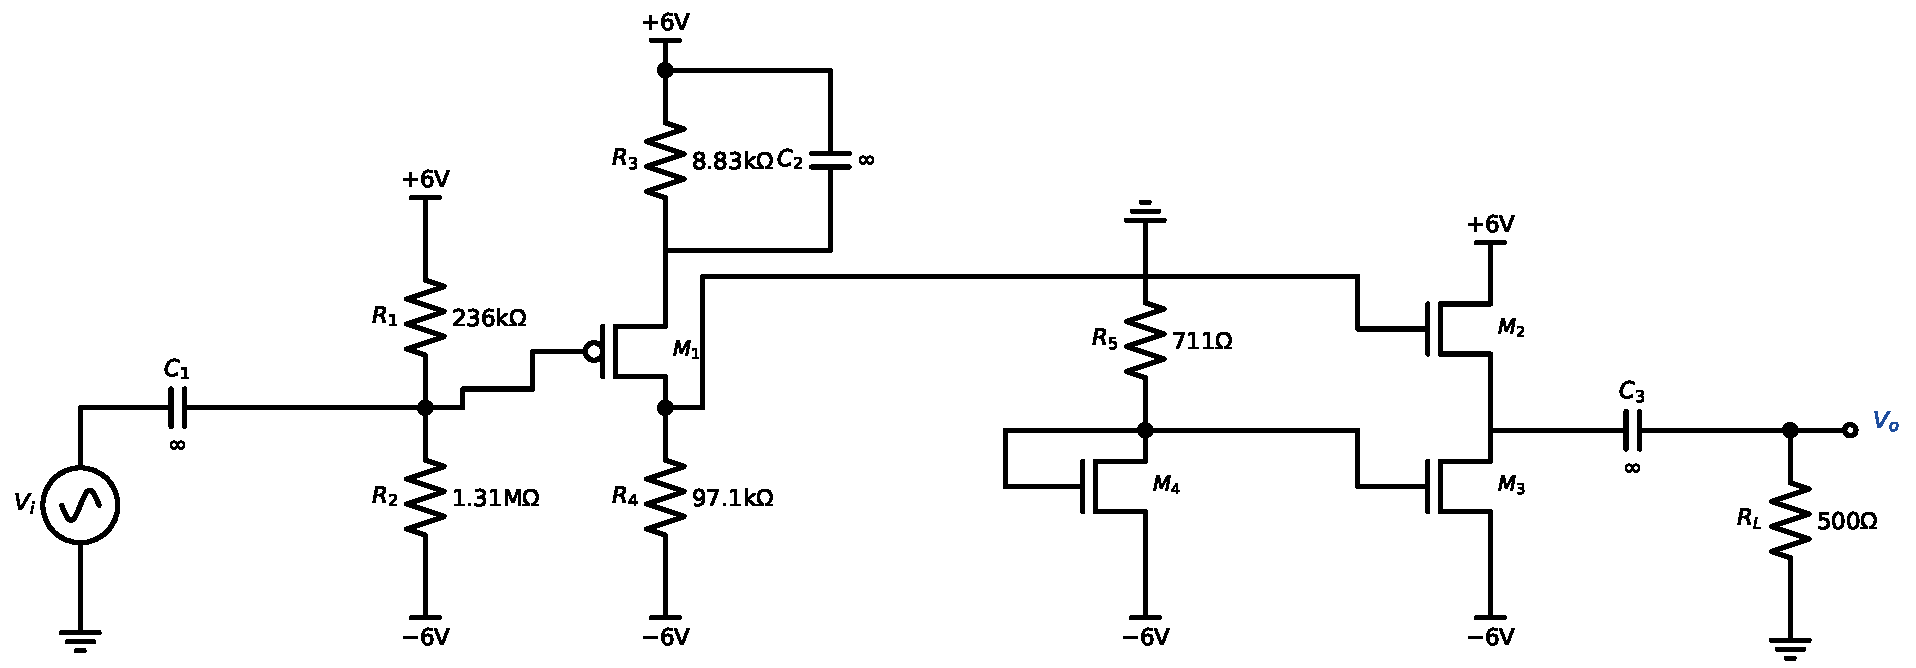
\includegraphics[width=0.85\linewidth,height=6cm,keepaspectratio]{p08_designed}\end{center}

\begin{ansbox}
$R_{1} = 236\,\mathrm{k}\Omega$,\quad $R_{2} = 1.31\,\mathrm{M}\Omega$,\quad $R_{3} = 8.83\,\mathrm{k}\Omega$,\quad $R_{4} = 97.1\,\mathrm{k}\Omega$,\quad $R_{5} = 711\,\Omega$
\end{ansbox}

\newpage
\subsection*{Solution 5E.9 \hfill Medium}
\begin{center}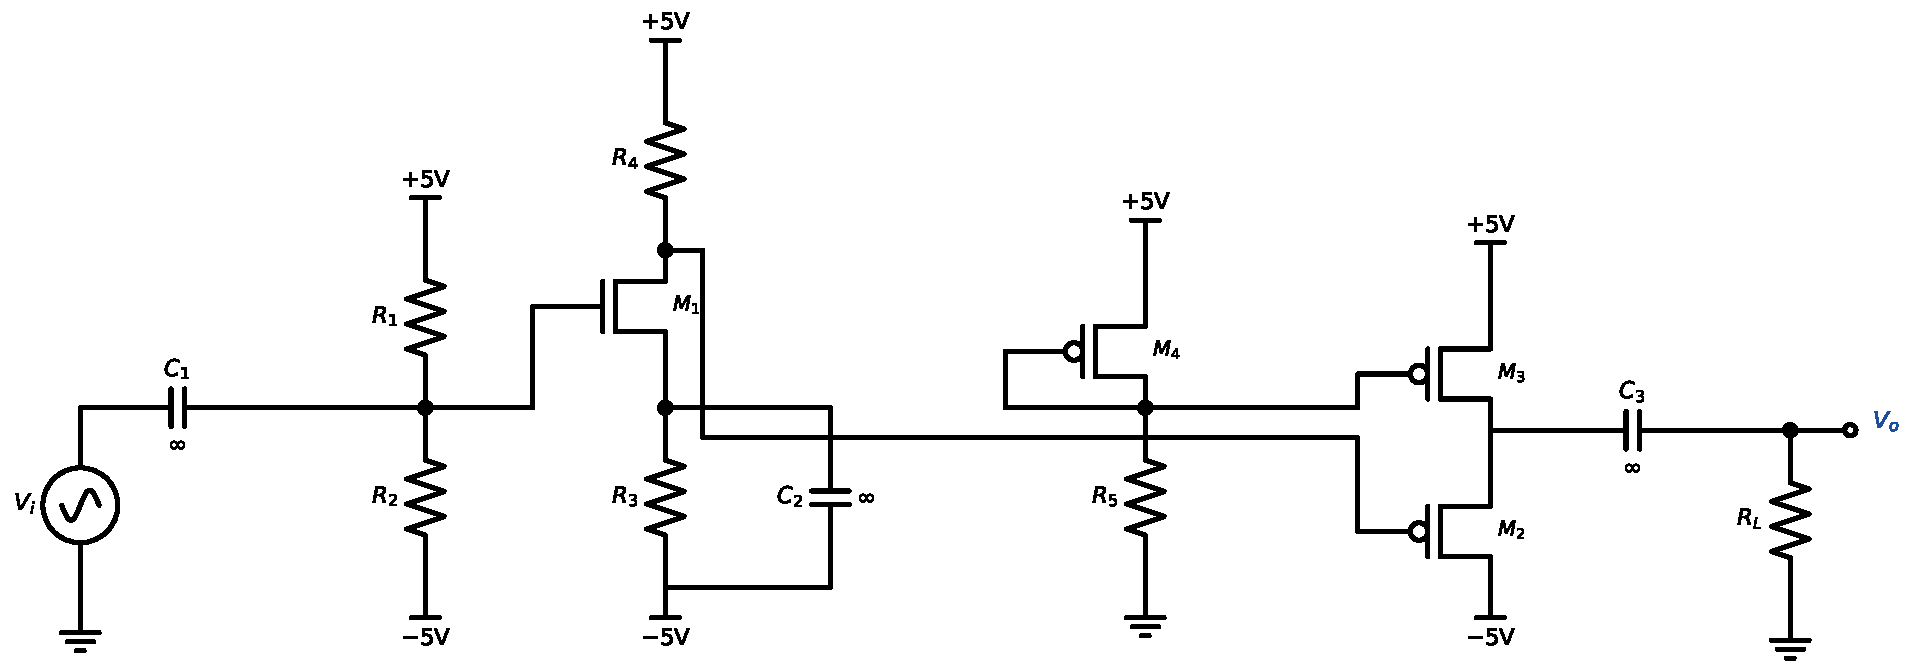
\includegraphics[width=0.9\linewidth,height=6cm,keepaspectratio]{p09_circuit}\end{center}
\solstep{1}{Plan}Follow the procedure of Sample Problem 5: size the output current sink for the load current, then the follower; budget the supply voltage around the drain swing; get $V_{ov1}$ from the gain ($|A_v| = g_mR = 2V_R/V_{ov}$), then the resistors; finally the gate divider from the input resistance. Distortion of a common-source stage: $HD_2 \approx \frac{\hat v_{gs}}{4V_{ov}}$ (from $i_D = \frac{k}{2}(V_{ov} + v_{gs})^2$).
\solstep{2}{Output stage: sink, reference and follower}The sink $M_3$ must deliver the whole peak load current: $I_{D3} \ge \frac{\hat V_o}{R_L} = \frac{1.5}{100\,\Omega} = 15\,\mathrm{m}\mathrm{A}$; use $I_{D3} = 20\,\mathrm{m}\mathrm{A}$ (given). Then $\frac{k_3}{2}V_{ov3}^2 = I_{D3} \Rightarrow V_{ov3} = \sqrt{\frac{2\cdot20\,\mathrm{m}\mathrm{A}}{40\,\mathrm{m}\mathrm{A/V^2}}} = 1$\,V.

$M_4$ is identical to $M_3$ and has the same $V_{GS}$, so $I_{D4} = I_{D3}$ and $V_{ov4} = V_{ov3}$.

\[R_5 = \frac{5 - |V_{t}| - V_{ov4}}{I_{D4}} = \frac{5 - 1.5 - 1}{20\,\mathrm{m}\mathrm{A}} = \mathbf{125\,\Omega}\]

The follower $M_2$ carries the same current, $I_{D2} = I_{D3}$, so $V_{ov2} = 1$\,V, $g_{m2} = k_2V_{ov2} = 40\,\mathrm{m}\mathrm{A/V}$, $1/g_{m2} = 25\,\Omega$ and (the sink $M_3$ is a current source, $Z = \infty$) \[A_{v2} = \frac{R_L}{1/g_{m2} + R_L} = \frac{100\,\Omega}{25\,\Omega + 100\,\Omega} = 0.8\]So the drain of $M_1$ must swing $\hat V_d = \hat V_o/A_{v2} = 1.875$\,V and $|A_{v1}| = |A_v|/A_{v2} = 31.25$.
\solstep{3}{Common-source stage}Voltage budget of the $V_{DD} + V_{SS} = 10$\,V branch through $R_3$, $M_1$, $R_4$. At the highest drain voltage of $M_1$ the follower and the sink must both stay active (the drain of $M_1$ sits one $|V_{GS2}|$ away from the output, which needs $V_{ov3}$ of room above the rail): \[V_{R4} \ge V_{ov3} + V_{ov2} + |V_{t2}| + \hat V_d = 1 + 1 + 1.5 + 1.88 = 5.375\,\mathrm{V}\]$M_1$ must stay active at the other extreme: $V_{R3} + V_{ov1} + \hat V_d + V_{R4} \le 10$, and with $V_{ov1} = 2V_{R4}/|A_{v1}|$ (below): \[V_{R4}\left(1 + \frac{2}{|A_{v1}|}\right) \le 10 - V_{R3} - \hat V_d \Rightarrow V_{R4} \le 7.166\,\mathrm{V}\]$V_{R3} = 0.5$\,V (its minimum) and $V_{R4} = 5.5$\,V (the next multiple of $0.5$\,V above the lower bound).

Gain of the common-source stage ($R_3$ is bypassed, the follower's gate loads nothing): \[|A_{v1}| = g_{m1}R_4 = k_1V_{ov1}\frac{V_{R4}}{\frac{k_1}{2}V_{ov1}^2} = \frac{2V_{R4}}{V_{ov1}} \Rightarrow V_{ov1} = \frac{2\cdot5.5}{31.25} = 0.352\,\mathrm{V}\]$I_{D1} = \frac{k_1}{2}V_{ov1}^2 = 124\,\mu \mathrm{A}$, $R_4 = \frac{V_{R4}}{I_{D1}} = \mathbf{44.4\,\mathrm{k}\Omega}$, $R_3 = \frac{V_{R3}}{I_{D1}} = \mathbf{4.04\,\mathrm{k}\Omega}$.

Gate divider: the resistor on the source side of $M_1$ carries $V_{R2} = V_{R3} + |V_{t1}| + V_{ov1} = 1.852$\,V, the other one $V_{R1} = 10 - 1.852 = 8.148$\,V. Both carry the same current ($I_G = 0$): $R_{2} = 1.852X$, $R_{1} = 8.148X$, and the input resistance is their parallel combination: \[R_1\|R_2 = \frac{1.852\cdot8.148}{10}X \ge 50\,\mathrm{k}\Omega \Rightarrow X = 33.1\,\mathrm{k}\Omega:\quad \mathbf{R_1 = 270\,\mathrm{k}\Omega},\ \mathbf{R_2 = 61.4\,\mathrm{k}\Omega}\]
\solstep{4}{Check by analysis}DC analysis of the finished circuit (as in sets 5A/5B):\begin{center}\renewcommand{\arraystretch}{1.35}
\begin{tabular}{cccc}
\toprule
 & $I_D$ & $V_{ov}$ & $|V_{DS}|$ \\
\midrule
$M_{1}$ & $124\,\mu \mathrm{A}$ & $0.352$\,V & $4$\,V \\
$M_{4}$ & $20\,\mathrm{m}\mathrm{A}$ & $1$\,V & $2.5$\,V \\
$M_{3}$ & $20\,\mathrm{m}\mathrm{A}$ & $1$\,V & $3$\,V \\
$M_{2}$ & $20\,\mathrm{m}\mathrm{A}$ & $1$\,V & $7$\,V \\
\bottomrule
\end{tabular}\end{center}
\begin{itemize}[leftmargin=*,itemsep=2pt]
\item $V_{DS1} = V_{D1} - V_{S1} = -0.5 - (-4.5) = 4\,\mathrm{V}$ $\ge V_{ov1} = 0.352$\,V $\Rightarrow$ $M_{1}$ is active \checkmark
\item $M_{4}$ is diode-connected: $V_{SD4} = V_{SG4} > V_{ov4}$, always active \checkmark
\item $V_{SD3} = 5 - V_{D3} = 5 - 2 = 3\,\mathrm{V}$ $\ge V_{ov3} = 1$\,V $\Rightarrow$ $M_{3}$ is active \checkmark
\item $V_{SD2} = V_{D3} - (-5) = 2 - (-5) = 7\,\mathrm{V}$ $\ge V_{ov2} = 1$\,V $\Rightarrow$ $M_{2}$ is active \checkmark
\item Gain (exact small-signal analysis of the finished circuit): $|A_v| = 25$ \checkmark
\item Input resistance $R_1\|R_2 = 50\,\mathrm{k}\Omega \ge 50\,\mathrm{k}\Omega$ \checkmark
\item Output swing before clipping: $M_1$ leaves saturation at $\hat V_o = 2.92$\,V; $M_3$ leaves saturation at $\hat V_o = 2$\,V; $M_2$ leaves saturation at $\hat V_o = 6$\,V; $M_3$ cannot sink more current (current clipping) at $\hat V_o = 2$\,V. The smallest is $2$\,V $\ge 1.5$\,V \checkmark
\item THD $\approx HD_2 = \frac{\hat v_{gs1}}{4V_{ov1}} = \frac{1.5/25}{4\cdot0.352} = 4.3\,\%$ $\le 10\,\%$ \checkmark
\end{itemize}

\begin{center}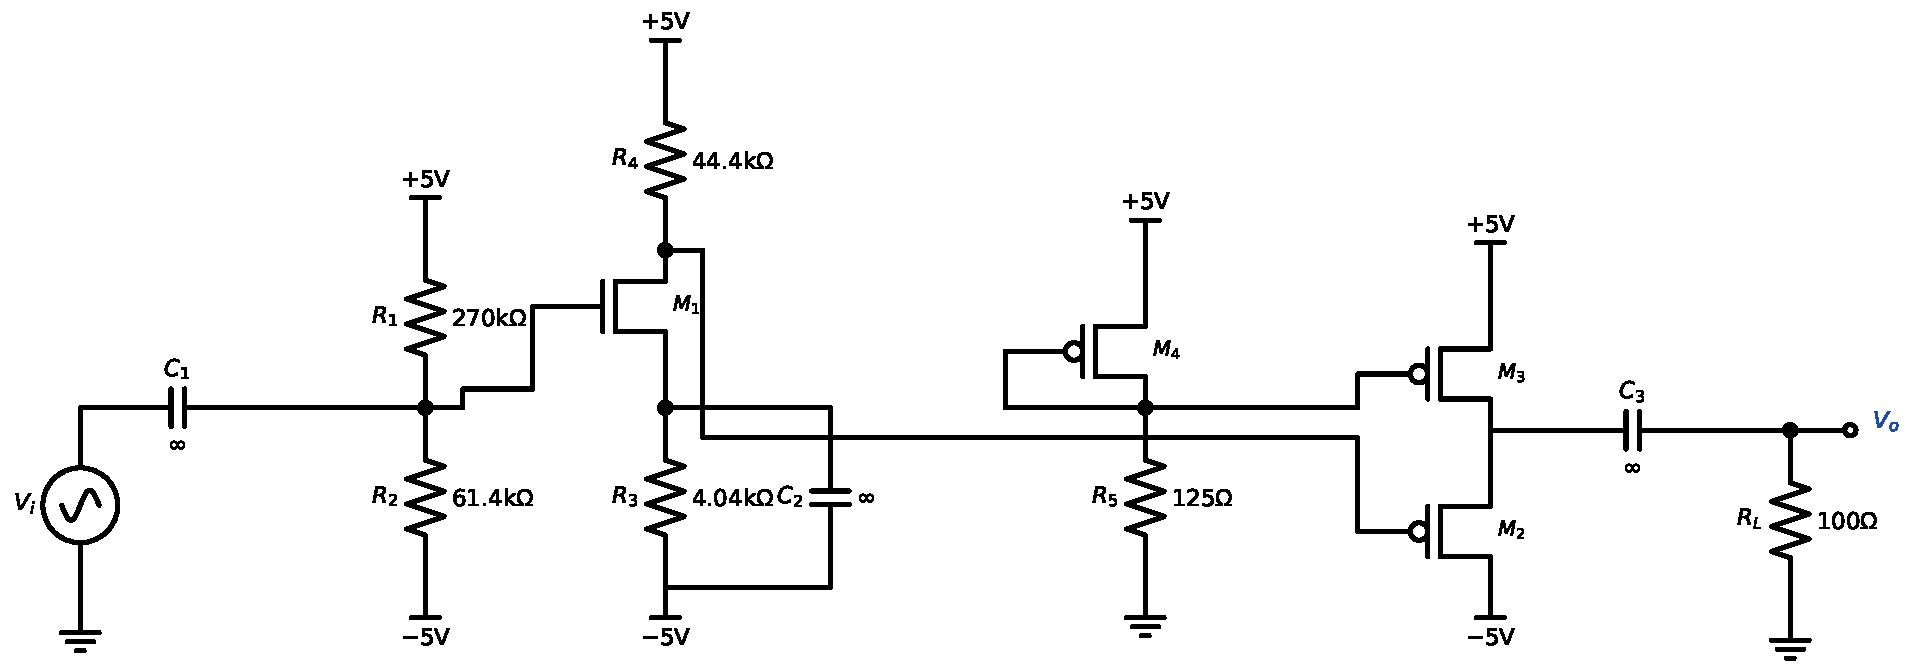
\includegraphics[width=0.85\linewidth,height=6cm,keepaspectratio]{p09_designed}\end{center}

\begin{ansbox}
$R_{1} = 270\,\mathrm{k}\Omega$,\quad $R_{2} = 61.4\,\mathrm{k}\Omega$,\quad $R_{3} = 4.04\,\mathrm{k}\Omega$,\quad $R_{4} = 44.4\,\mathrm{k}\Omega$,\quad $R_{5} = 125\,\Omega$
\end{ansbox}

\newpage
\subsection*{Solution 5E.10 \hfill Medium}
\begin{center}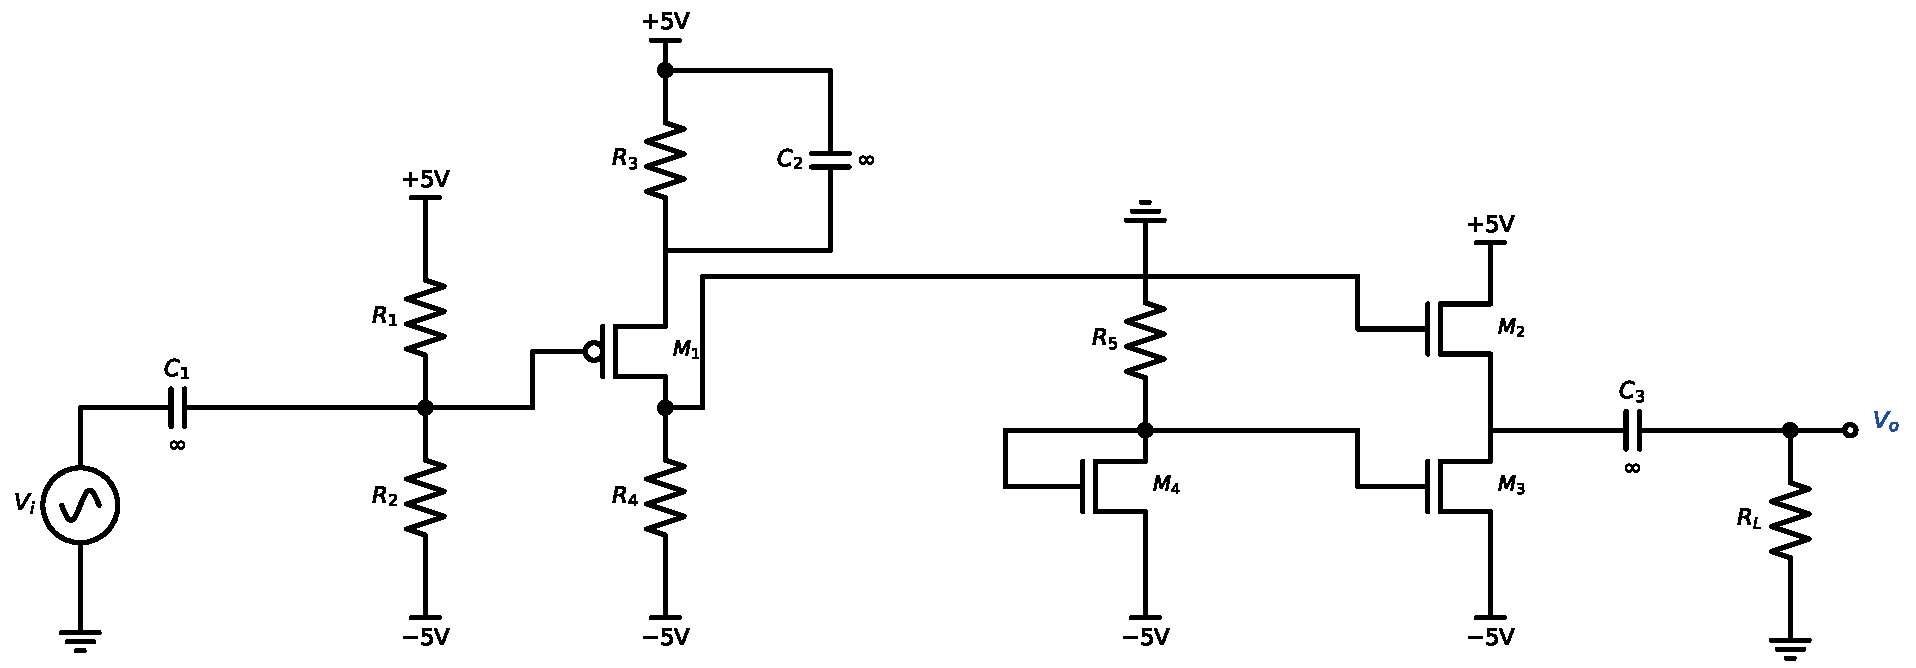
\includegraphics[width=0.9\linewidth,height=6cm,keepaspectratio]{p10_circuit}\end{center}
\solstep{1}{Plan}Follow the procedure of Sample Problem 5: size the output current sink for the load current, then the follower; budget the supply voltage around the drain swing; get $V_{ov1}$ from the gain ($|A_v| = g_mR = 2V_R/V_{ov}$), then the resistors; finally the gate divider from the input resistance. Distortion of a common-source stage: $HD_2 \approx \frac{\hat v_{gs}}{4V_{ov}}$ (from $i_D = \frac{k}{2}(V_{ov} + v_{gs})^2$).
\solstep{2}{Output stage: sink, reference and follower}The sink $M_3$ must deliver the whole peak load current: $I_{D3} \ge \frac{\hat V_o}{R_L} = \frac{1}{50\,\Omega} = 20\,\mathrm{m}\mathrm{A}$; use $I_{D3} = 25\,\mathrm{m}\mathrm{A}$ (given). Then $\frac{k_3}{2}V_{ov3}^2 = I_{D3} \Rightarrow V_{ov3} = \sqrt{\frac{2\cdot25\,\mathrm{m}\mathrm{A}}{50\,\mathrm{m}\mathrm{A/V^2}}} = 1$\,V.

$M_4$ is identical to $M_3$ and has the same $V_{GS}$, so $I_{D4} = I_{D3}$ and $V_{ov4} = V_{ov3}$.

\[R_5 = \frac{5 - |V_{t}| - V_{ov4}}{I_{D4}} = \frac{5 - 2 - 1}{25\,\mathrm{m}\mathrm{A}} = \mathbf{80\,\Omega}\]

The follower $M_2$ carries the same current, $I_{D2} = I_{D3}$, so $V_{ov2} = 1$\,V, $g_{m2} = k_2V_{ov2} = 50\,\mathrm{m}\mathrm{A/V}$, $1/g_{m2} = 20\,\Omega$ and (the sink $M_3$ is a current source, $Z = \infty$) \[A_{v2} = \frac{R_L}{1/g_{m2} + R_L} = \frac{50\,\Omega}{20\,\Omega + 50\,\Omega} = 0.7143\]So the drain of $M_1$ must swing $\hat V_d = \hat V_o/A_{v2} = 1.4$\,V and $|A_{v1}| = |A_v|/A_{v2} = 21$.
\solstep{3}{Common-source stage}Voltage budget of the $V_{DD} + V_{SS} = 10$\,V branch through $R_3$, $M_1$, $R_4$. At the lowest drain voltage of $M_1$ the follower and the sink must both stay active (the drain of $M_1$ sits one $|V_{GS2}|$ away from the output, which needs $V_{ov3}$ of room above the rail): \[V_{R4} \ge V_{ov3} + V_{ov2} + |V_{t2}| + \hat V_d = 1 + 1 + 2 + 1.4 = 5.4\,\mathrm{V}\]$M_1$ must stay active at the other extreme: $V_{R3} + V_{ov1} + \hat V_d + V_{R4} \le 10$, and with $V_{ov1} = 2V_{R4}/|A_{v1}|$ (below): \[V_{R4}\left(1 + \frac{2}{|A_{v1}|}\right) \le 10 - V_{R3} - \hat V_d \Rightarrow V_{R4} \le 7.396\,\mathrm{V}\]$V_{R3} = 0.5$\,V (its minimum) and $V_{R4} = 5.5$\,V (the next multiple of $0.5$\,V above the lower bound).

Gain of the common-source stage ($R_3$ is bypassed, the follower's gate loads nothing): \[|A_{v1}| = g_{m1}R_4 = k_1V_{ov1}\frac{V_{R4}}{\frac{k_1}{2}V_{ov1}^2} = \frac{2V_{R4}}{V_{ov1}} \Rightarrow V_{ov1} = \frac{2\cdot5.5}{21} = 0.5238\,\mathrm{V}\]$I_{D1} = \frac{k_1}{2}V_{ov1}^2 = 137\,\mu \mathrm{A}$, $R_4 = \frac{V_{R4}}{I_{D1}} = \mathbf{40.1\,\mathrm{k}\Omega}$, $R_3 = \frac{V_{R3}}{I_{D1}} = \mathbf{3.64\,\mathrm{k}\Omega}$.

Gate divider: the resistor on the source side of $M_1$ carries $V_{R1} = V_{R3} + |V_{t1}| + V_{ov1} = 2.024$\,V, the other one $V_{R2} = 10 - 2.024 = 7.976$\,V. Both carry the same current ($I_G = 0$): $R_{1} = 2.024X$, $R_{2} = 7.976X$, and the input resistance is their parallel combination: \[R_1\|R_2 = \frac{2.024\cdot7.976}{10}X \ge 100\,\mathrm{k}\Omega \Rightarrow X = 61.9\,\mathrm{k}\Omega:\quad \mathbf{R_1 = 125\,\mathrm{k}\Omega},\ \mathbf{R_2 = 494\,\mathrm{k}\Omega}\]
\solstep{4}{Check by analysis}DC analysis of the finished circuit (as in sets 5A/5B):\begin{center}\renewcommand{\arraystretch}{1.35}
\begin{tabular}{cccc}
\toprule
 & $I_D$ & $V_{ov}$ & $|V_{DS}|$ \\
\midrule
$M_{1}$ & $137\,\mu \mathrm{A}$ & $0.524$\,V & $4$\,V \\
$M_{4}$ & $25\,\mathrm{m}\mathrm{A}$ & $1$\,V & $3$\,V \\
$M_{2}$ & $25\,\mathrm{m}\mathrm{A}$ & $1$\,V & $7.5$\,V \\
$M_{3}$ & $25\,\mathrm{m}\mathrm{A}$ & $1$\,V & $2.5$\,V \\
\bottomrule
\end{tabular}\end{center}
\begin{itemize}[leftmargin=*,itemsep=2pt]
\item $V_{SD1} = V_{S1} - V_{D1} = 4.5 - 0.5 = 4\,\mathrm{V}$ $\ge V_{ov1} = 0.524$\,V $\Rightarrow$ $M_{1}$ is active \checkmark
\item $M_{4}$ is diode-connected: $V_{DS4} = V_{GS4} > V_{ov4}$, always active \checkmark
\item $V_{DS2} = 5 - V_{S2} = 5 - (-2.5) = 7.5\,\mathrm{V}$ $\ge V_{ov2} = 1$\,V $\Rightarrow$ $M_{2}$ is active \checkmark
\item $V_{DS3} = V_{S2} - (-5) = -2.5 - (-5) = 2.5\,\mathrm{V}$ $\ge V_{ov3} = 1$\,V $\Rightarrow$ $M_{3}$ is active \checkmark
\item Gain (exact small-signal analysis of the finished circuit): $|A_v| = 15$ \checkmark
\item Input resistance $R_1\|R_2 = 100\,\mathrm{k}\Omega \ge 100\,\mathrm{k}\Omega$ \checkmark
\item Output swing before clipping: $M_1$ leaves saturation at $\hat V_o = 2.48$\,V; $M_3$ leaves saturation at $\hat V_o = 1.5$\,V; $M_2$ leaves saturation at $\hat V_o = 6.5$\,V; $M_3$ cannot sink more current (current clipping) at $\hat V_o = 1.25$\,V. The smallest is $1.25$\,V $\ge 1$\,V \checkmark
\item THD $\approx HD_2 = \frac{\hat v_{gs1}}{4V_{ov1}} = \frac{1/15}{4\cdot0.524} = 3.2\,\%$ $\le 10\,\%$ \checkmark
\end{itemize}

\begin{center}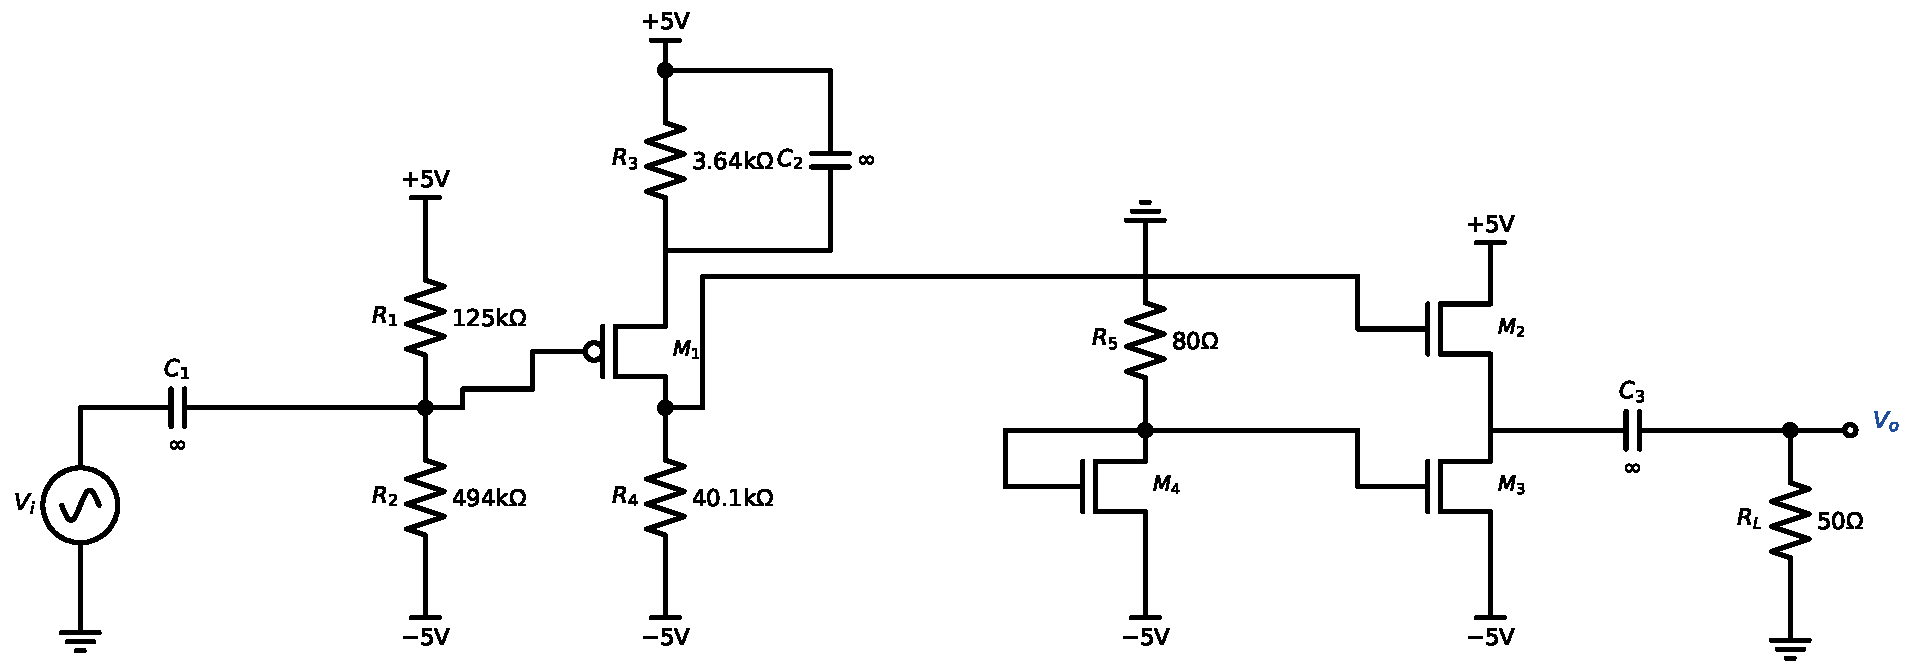
\includegraphics[width=0.85\linewidth,height=6cm,keepaspectratio]{p10_designed}\end{center}

\begin{ansbox}
$R_{1} = 125\,\mathrm{k}\Omega$,\quad $R_{2} = 494\,\mathrm{k}\Omega$,\quad $R_{3} = 3.64\,\mathrm{k}\Omega$,\quad $R_{4} = 40.1\,\mathrm{k}\Omega$,\quad $R_{5} = 80\,\Omega$
\end{ansbox}

\newpage
\subsection*{Solution 5E.11 \hfill Medium}
\begin{center}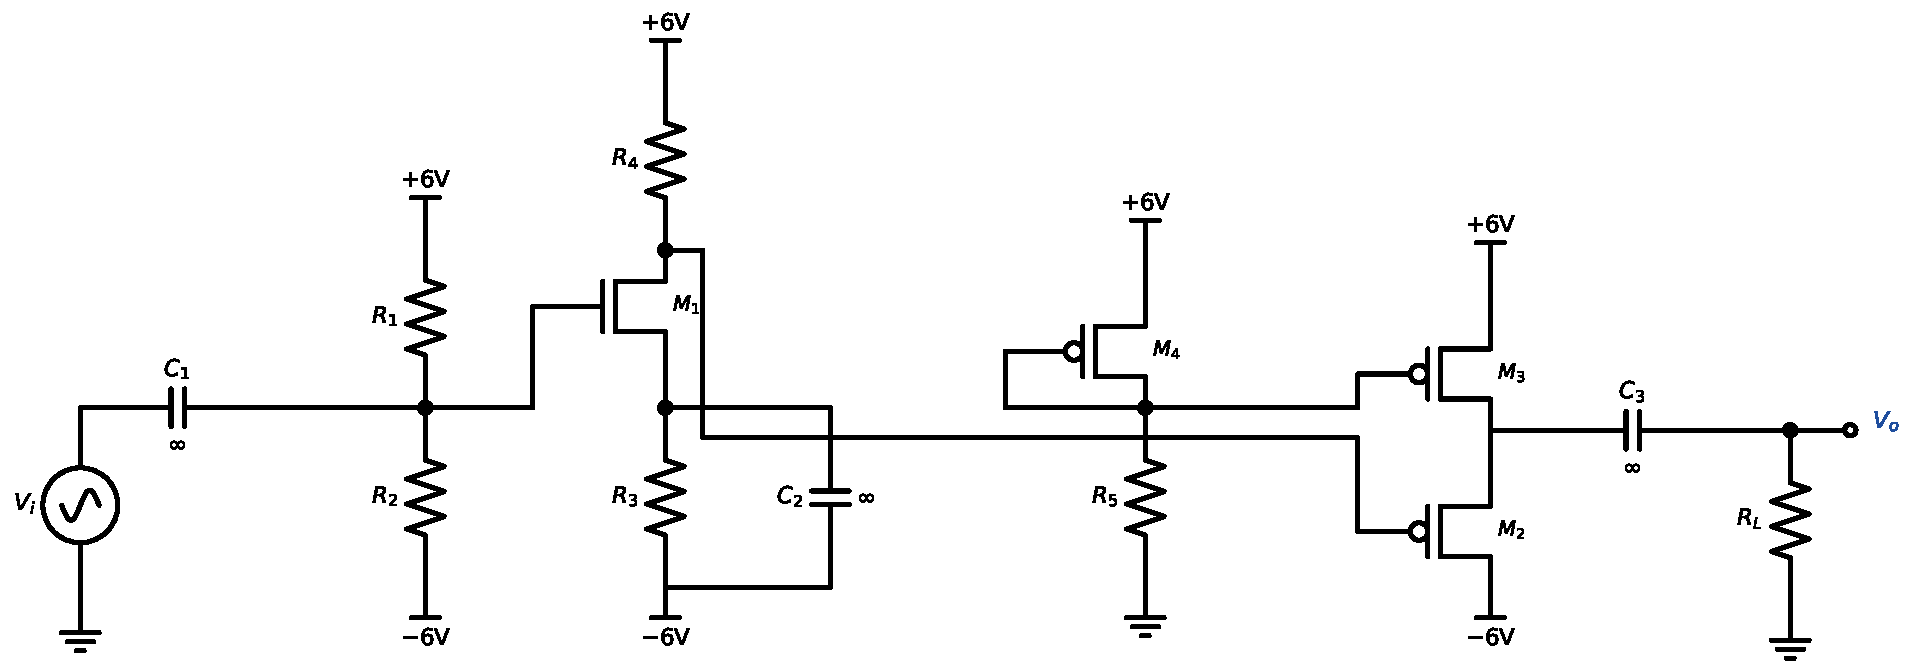
\includegraphics[width=0.9\linewidth,height=6cm,keepaspectratio]{p11_circuit}\end{center}
\solstep{1}{Plan}Follow the procedure of Sample Problem 5: size the output current sink for the load current, then the follower; budget the supply voltage around the drain swing; get $V_{ov1}$ from the gain ($|A_v| = g_mR = 2V_R/V_{ov}$), then the resistors; finally the gate divider from the input resistance. Distortion of a common-source stage: $HD_2 \approx \frac{\hat v_{gs}}{4V_{ov}}$ (from $i_D = \frac{k}{2}(V_{ov} + v_{gs})^2$).
\solstep{2}{Output stage: sink, reference and follower}The sink $M_3$ must deliver the whole peak load current: $I_{D3} \ge \frac{\hat V_o}{R_L} = \frac{2}{200\,\Omega} = 10\,\mathrm{m}\mathrm{A}$; use $I_{D3} = 12\,\mathrm{m}\mathrm{A}$ (given). Then $\frac{k_3}{2}V_{ov3}^2 = I_{D3} \Rightarrow V_{ov3} = \sqrt{\frac{2\cdot12\,\mathrm{m}\mathrm{A}}{50\,\mathrm{m}\mathrm{A/V^2}}} = 0.6928$\,V.

$M_4$ is identical to $M_3$ and has the same $V_{GS}$, so $I_{D4} = I_{D3}$ and $V_{ov4} = V_{ov3}$.

\[R_5 = \frac{6 - |V_{t}| - V_{ov4}}{I_{D4}} = \frac{6 - 1.5 - 0.6928}{12\,\mathrm{m}\mathrm{A}} = \mathbf{317\,\Omega}\]

The follower $M_2$ carries the same current, $I_{D2} = I_{D3}$, so $V_{ov2} = 0.6928$\,V, $g_{m2} = k_2V_{ov2} = 34.6\,\mathrm{m}\mathrm{A/V}$, $1/g_{m2} = 28.9\,\Omega$ and (the sink $M_3$ is a current source, $Z = \infty$) \[A_{v2} = \frac{R_L}{1/g_{m2} + R_L} = \frac{200\,\Omega}{28.9\,\Omega + 200\,\Omega} = 0.8739\]So the drain of $M_1$ must swing $\hat V_d = \hat V_o/A_{v2} = 2.289$\,V and $|A_{v1}| = |A_v|/A_{v2} = 22.89$.
\solstep{3}{Common-source stage}Voltage budget of the $V_{DD} + V_{SS} = 12$\,V branch through $R_3$, $M_1$, $R_4$. At the highest drain voltage of $M_1$ the follower and the sink must both stay active (the drain of $M_1$ sits one $|V_{GS2}|$ away from the output, which needs $V_{ov3}$ of room above the rail): \[V_{R4} \ge V_{ov3} + V_{ov2} + |V_{t2}| + \hat V_d = 0.693 + 0.693 + 1.5 + 2.29 = 5.174\,\mathrm{V}\]$M_1$ must stay active at the other extreme: $V_{R3} + V_{ov1} + \hat V_d + V_{R4} \le 12$, and with $V_{ov1} = 2V_{R4}/|A_{v1}|$ (below): \[V_{R4}\left(1 + \frac{2}{|A_{v1}|}\right) \le 12 - V_{R3} - \hat V_d \Rightarrow V_{R4} \le 8.471\,\mathrm{V}\]$V_{R3} = 0.5$\,V (its minimum) and $V_{R4} = 5.5$\,V (the next multiple of $0.5$\,V above the lower bound).

Gain of the common-source stage ($R_3$ is bypassed, the follower's gate loads nothing): \[|A_{v1}| = g_{m1}R_4 = k_1V_{ov1}\frac{V_{R4}}{\frac{k_1}{2}V_{ov1}^2} = \frac{2V_{R4}}{V_{ov1}} \Rightarrow V_{ov1} = \frac{2\cdot5.5}{22.89} = 0.4806\,\mathrm{V}\]$I_{D1} = \frac{k_1}{2}V_{ov1}^2 = 116\,\mu \mathrm{A}$, $R_4 = \frac{V_{R4}}{I_{D1}} = \mathbf{47.6\,\mathrm{k}\Omega}$, $R_3 = \frac{V_{R3}}{I_{D1}} = \mathbf{4.33\,\mathrm{k}\Omega}$.

Gate divider: the resistor on the source side of $M_1$ carries $V_{R2} = V_{R3} + |V_{t1}| + V_{ov1} = 1.981$\,V, the other one $V_{R1} = 12 - 1.981 = 10.02$\,V. Both carry the same current ($I_G = 0$): $R_{2} = 1.981X$, $R_{1} = 10.02X$, and the input resistance is their parallel combination: \[R_1\|R_2 = \frac{1.981\cdot10.02}{12}X \ge 100\,\mathrm{k}\Omega \Rightarrow X = 60.5\,\mathrm{k}\Omega:\quad \mathbf{R_1 = 606\,\mathrm{k}\Omega},\ \mathbf{R_2 = 120\,\mathrm{k}\Omega}\]
\solstep{4}{Check by analysis}DC analysis of the finished circuit (as in sets 5A/5B):\begin{center}\renewcommand{\arraystretch}{1.35}
\begin{tabular}{cccc}
\toprule
 & $I_D$ & $V_{ov}$ & $|V_{DS}|$ \\
\midrule
$M_{1}$ & $116\,\mu \mathrm{A}$ & $0.481$\,V & $6$\,V \\
$M_{4}$ & $12\,\mathrm{m}\mathrm{A}$ & $0.693$\,V & $2.193$\,V \\
$M_{3}$ & $12\,\mathrm{m}\mathrm{A}$ & $0.693$\,V & $3.307$\,V \\
$M_{2}$ & $12\,\mathrm{m}\mathrm{A}$ & $0.693$\,V & $8.693$\,V \\
\bottomrule
\end{tabular}\end{center}
\begin{itemize}[leftmargin=*,itemsep=2pt]
\item $V_{DS1} = V_{D1} - V_{S1} = 0.5 - (-5.5) = 6\,\mathrm{V}$ $\ge V_{ov1} = 0.481$\,V $\Rightarrow$ $M_{1}$ is active \checkmark
\item $M_{4}$ is diode-connected: $V_{SD4} = V_{SG4} > V_{ov4}$, always active \checkmark
\item $V_{SD3} = 6 - V_{D3} = 6 - 2.693 = 3.31\,\mathrm{V}$ $\ge V_{ov3} = 0.693$\,V $\Rightarrow$ $M_{3}$ is active \checkmark
\item $V_{SD2} = V_{D3} - (-6) = 2.693 - (-6) = 8.69\,\mathrm{V}$ $\ge V_{ov2} = 0.693$\,V $\Rightarrow$ $M_{2}$ is active \checkmark
\item Gain (exact small-signal analysis of the finished circuit): $|A_v| = 20$ \checkmark
\item Input resistance $R_1\|R_2 = 100\,\mathrm{k}\Omega \ge 100\,\mathrm{k}\Omega$ \checkmark
\item Output swing before clipping: $M_1$ leaves saturation at $\hat V_o = 4.82$\,V; $M_3$ leaves saturation at $\hat V_o = 2.61$\,V; $M_2$ leaves saturation at $\hat V_o = 8$\,V; $M_3$ cannot sink more current (current clipping) at $\hat V_o = 2.4$\,V. The smallest is $2.4$\,V $\ge 2$\,V \checkmark
\item THD $\approx HD_2 = \frac{\hat v_{gs1}}{4V_{ov1}} = \frac{2/20}{4\cdot0.481} = 5.2\,\%$ $\le 10\,\%$ \checkmark
\end{itemize}

\begin{center}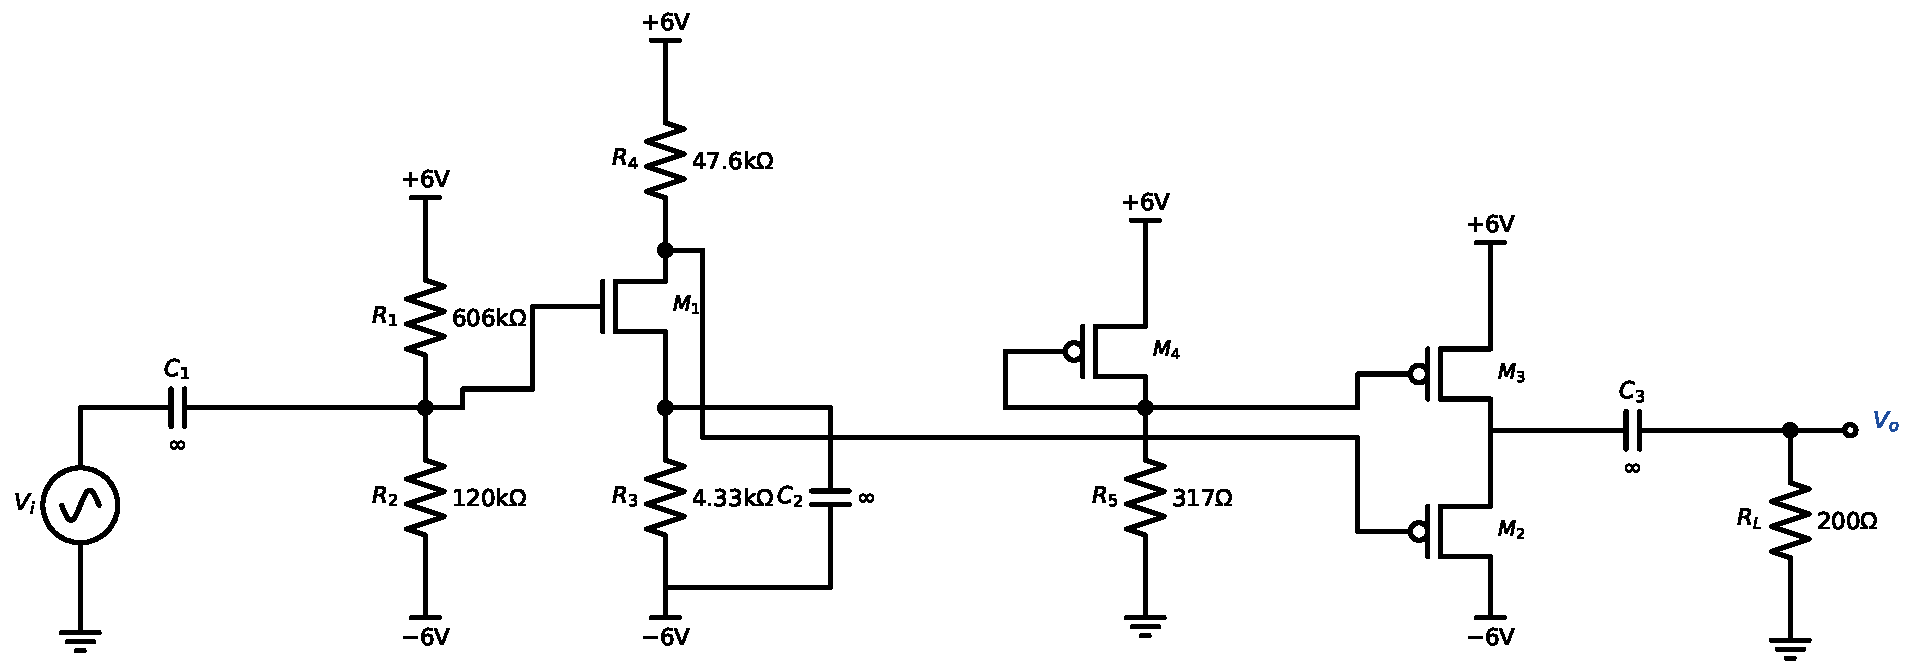
\includegraphics[width=0.85\linewidth,height=6cm,keepaspectratio]{p11_designed}\end{center}

\begin{ansbox}
$R_{1} = 606\,\mathrm{k}\Omega$,\quad $R_{2} = 120\,\mathrm{k}\Omega$,\quad $R_{3} = 4.33\,\mathrm{k}\Omega$,\quad $R_{4} = 47.6\,\mathrm{k}\Omega$,\quad $R_{5} = 317\,\Omega$
\end{ansbox}

\newpage
\subsection*{Solution 5E.12 \hfill Medium}
\begin{center}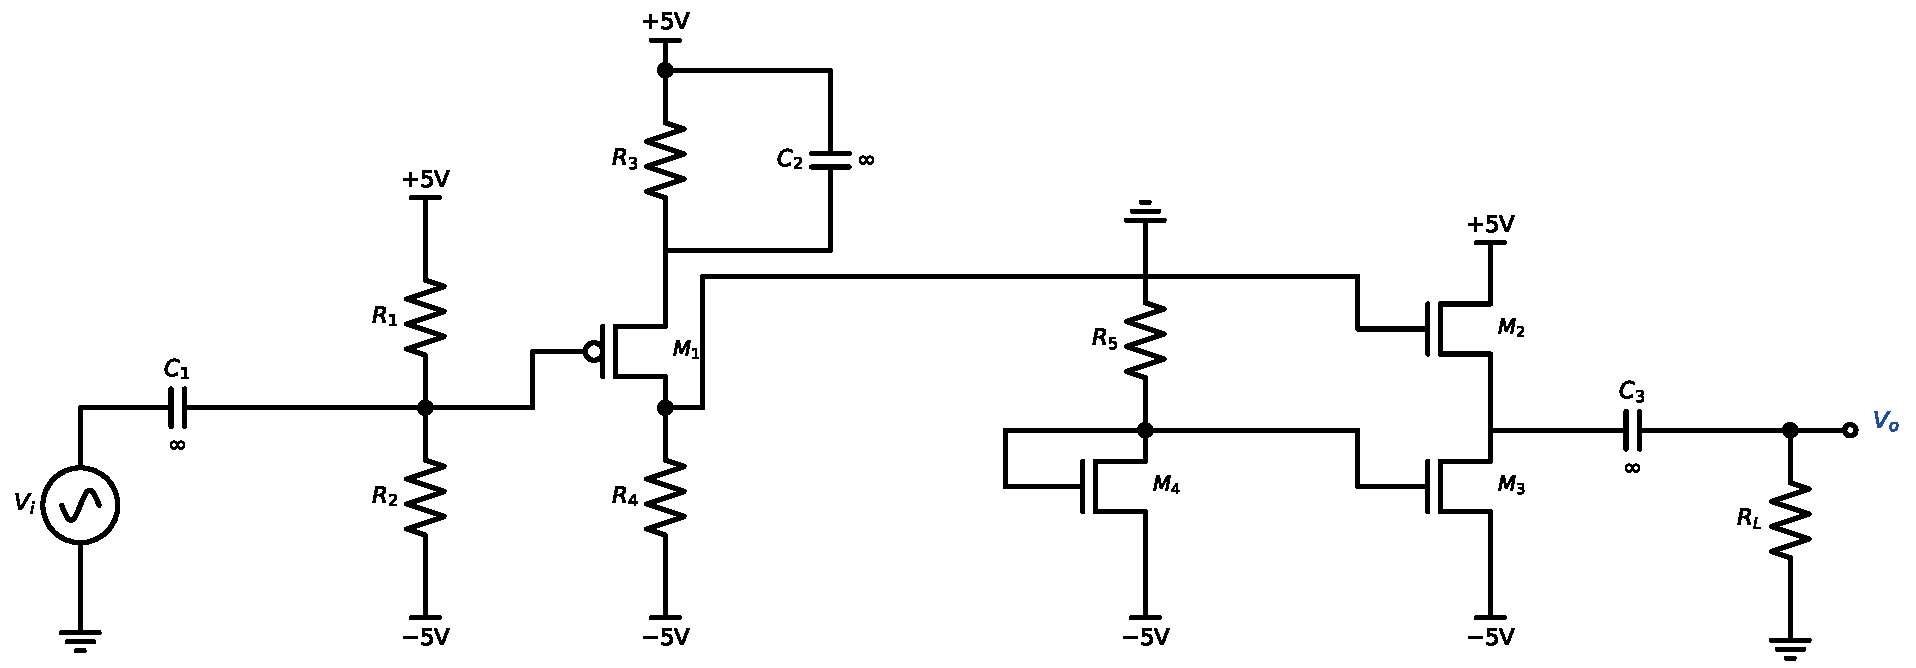
\includegraphics[width=0.9\linewidth,height=6cm,keepaspectratio]{p12_circuit}\end{center}
\solstep{1}{Plan}Follow the procedure of Sample Problem 5: size the output current sink for the load current, then the follower; budget the supply voltage around the drain swing; get $V_{ov1}$ from the gain ($|A_v| = g_mR = 2V_R/V_{ov}$), then the resistors; finally the gate divider from the input resistance. Distortion of a common-source stage: $HD_2 \approx \frac{\hat v_{gs}}{4V_{ov}}$ (from $i_D = \frac{k}{2}(V_{ov} + v_{gs})^2$).
\solstep{2}{Output stage: sink, reference and follower}The sink $M_3$ must deliver the whole peak load current: $I_{D3} \ge \frac{\hat V_o}{R_L} = \frac{1.5}{100\,\Omega} = 15\,\mathrm{m}\mathrm{A}$; use $I_{D3} = 20\,\mathrm{m}\mathrm{A}$ (given). Then $\frac{k_3}{2}V_{ov3}^2 = I_{D3} \Rightarrow V_{ov3} = \sqrt{\frac{2\cdot20\,\mathrm{m}\mathrm{A}}{50\,\mathrm{m}\mathrm{A/V^2}}} = 0.8944$\,V.

$M_4$ has the same $V_{GS}$ as $M_3$ but $k_4 = 0.2\,k_3$, so $I_{D4} = 0.2\,I_{D3} = 4\,\mathrm{m}\mathrm{A}$ (same $V_{ov}$).

\[R_5 = \frac{5 - |V_{t}| - V_{ov4}}{I_{D4}} = \frac{5 - 2 - 0.8944}{4\,\mathrm{m}\mathrm{A}} = \mathbf{526\,\Omega}\]

The follower $M_2$ carries the same current, $I_{D2} = I_{D3}$, so $V_{ov2} = 0.8944$\,V, $g_{m2} = k_2V_{ov2} = 44.7\,\mathrm{m}\mathrm{A/V}$, $1/g_{m2} = 22.4\,\Omega$ and (the sink $M_3$ is a current source, $Z = \infty$) \[A_{v2} = \frac{R_L}{1/g_{m2} + R_L} = \frac{100\,\Omega}{22.4\,\Omega + 100\,\Omega} = 0.8173\]So the drain of $M_1$ must swing $\hat V_d = \hat V_o/A_{v2} = 1.835$\,V and $|A_{v1}| = |A_v|/A_{v2} = 36.71$.
\solstep{3}{Common-source stage}Voltage budget of the $V_{DD} + V_{SS} = 10$\,V branch through $R_3$, $M_1$, $R_4$. At the lowest drain voltage of $M_1$ the follower and the sink must both stay active (the drain of $M_1$ sits one $|V_{GS2}|$ away from the output, which needs $V_{ov3}$ of room above the rail): \[V_{R4} \ge V_{ov3} + V_{ov2} + |V_{t2}| + \hat V_d = 0.894 + 0.894 + 2 + 1.84 = 5.624\,\mathrm{V}\]$M_1$ must stay active at the other extreme: $V_{R3} + V_{ov1} + \hat V_d + V_{R4} \le 10$, and with $V_{ov1} = 2V_{R4}/|A_{v1}|$ (below): \[V_{R4}\left(1 + \frac{2}{|A_{v1}|}\right) \le 10 - V_{R3} - \hat V_d \Rightarrow V_{R4} \le 7.269\,\mathrm{V}\]$V_{R3} = 0.5$\,V (its minimum) and $V_{R4} = 6$\,V (the next multiple of $0.5$\,V above the lower bound).

Gain of the common-source stage ($R_3$ is bypassed, the follower's gate loads nothing): \[|A_{v1}| = g_{m1}R_4 = k_1V_{ov1}\frac{V_{R4}}{\frac{k_1}{2}V_{ov1}^2} = \frac{2V_{R4}}{V_{ov1}} \Rightarrow V_{ov1} = \frac{2\cdot6}{36.71} = 0.3269\,\mathrm{V}\]$I_{D1} = \frac{k_1}{2}V_{ov1}^2 = 53.4\,\mu \mathrm{A}$, $R_4 = \frac{V_{R4}}{I_{D1}} = \mathbf{112\,\mathrm{k}\Omega}$, $R_3 = \frac{V_{R3}}{I_{D1}} = \mathbf{9.36\,\mathrm{k}\Omega}$.

Gate divider: the resistor on the source side of $M_1$ carries $V_{R1} = V_{R3} + |V_{t1}| + V_{ov1} = 1.827$\,V, the other one $V_{R2} = 10 - 1.827 = 8.173$\,V. Both carry the same current ($I_G = 0$): $R_{1} = 1.827X$, $R_{2} = 8.173X$, and the input resistance is their parallel combination: \[R_1\|R_2 = \frac{1.827\cdot8.173}{10}X \ge 100\,\mathrm{k}\Omega \Rightarrow X = 67\,\mathrm{k}\Omega:\quad \mathbf{R_1 = 122\,\mathrm{k}\Omega},\ \mathbf{R_2 = 547\,\mathrm{k}\Omega}\]
\solstep{4}{Check by analysis}DC analysis of the finished circuit (as in sets 5A/5B):\begin{center}\renewcommand{\arraystretch}{1.35}
\begin{tabular}{cccc}
\toprule
 & $I_D$ & $V_{ov}$ & $|V_{DS}|$ \\
\midrule
$M_{1}$ & $53.4\,\mu \mathrm{A}$ & $0.327$\,V & $3.5$\,V \\
$M_{4}$ & $4\,\mathrm{m}\mathrm{A}$ & $0.894$\,V & $2.894$\,V \\
$M_{2}$ & $20\,\mathrm{m}\mathrm{A}$ & $0.894$\,V & $6.894$\,V \\
$M_{3}$ & $20\,\mathrm{m}\mathrm{A}$ & $0.894$\,V & $3.106$\,V \\
\bottomrule
\end{tabular}\end{center}
\begin{itemize}[leftmargin=*,itemsep=2pt]
\item $V_{SD1} = V_{S1} - V_{D1} = 4.5 - 1 = 3.5\,\mathrm{V}$ $\ge V_{ov1} = 0.327$\,V $\Rightarrow$ $M_{1}$ is active \checkmark
\item $M_{4}$ is diode-connected: $V_{DS4} = V_{GS4} > V_{ov4}$, always active \checkmark
\item $V_{DS2} = 5 - V_{S2} = 5 - (-1.894) = 6.89\,\mathrm{V}$ $\ge V_{ov2} = 0.894$\,V $\Rightarrow$ $M_{2}$ is active \checkmark
\item $V_{DS3} = V_{S2} - (-5) = -1.894 - (-5) = 3.11\,\mathrm{V}$ $\ge V_{ov3} = 0.894$\,V $\Rightarrow$ $M_{3}$ is active \checkmark
\item Gain (exact small-signal analysis of the finished circuit): $|A_v| = 30$ \checkmark
\item Input resistance $R_1\|R_2 = 100\,\mathrm{k}\Omega \ge 100\,\mathrm{k}\Omega$ \checkmark
\item Output swing before clipping: $M_1$ leaves saturation at $\hat V_o = 2.59$\,V; $M_3$ leaves saturation at $\hat V_o = 2.21$\,V; $M_2$ leaves saturation at $\hat V_o = 6$\,V; $M_3$ cannot sink more current (current clipping) at $\hat V_o = 2$\,V. The smallest is $2$\,V $\ge 1.5$\,V \checkmark
\item THD $\approx HD_2 = \frac{\hat v_{gs1}}{4V_{ov1}} = \frac{1.5/30}{4\cdot0.327} = 3.8\,\%$ $\le 10\,\%$ \checkmark
\end{itemize}

\begin{center}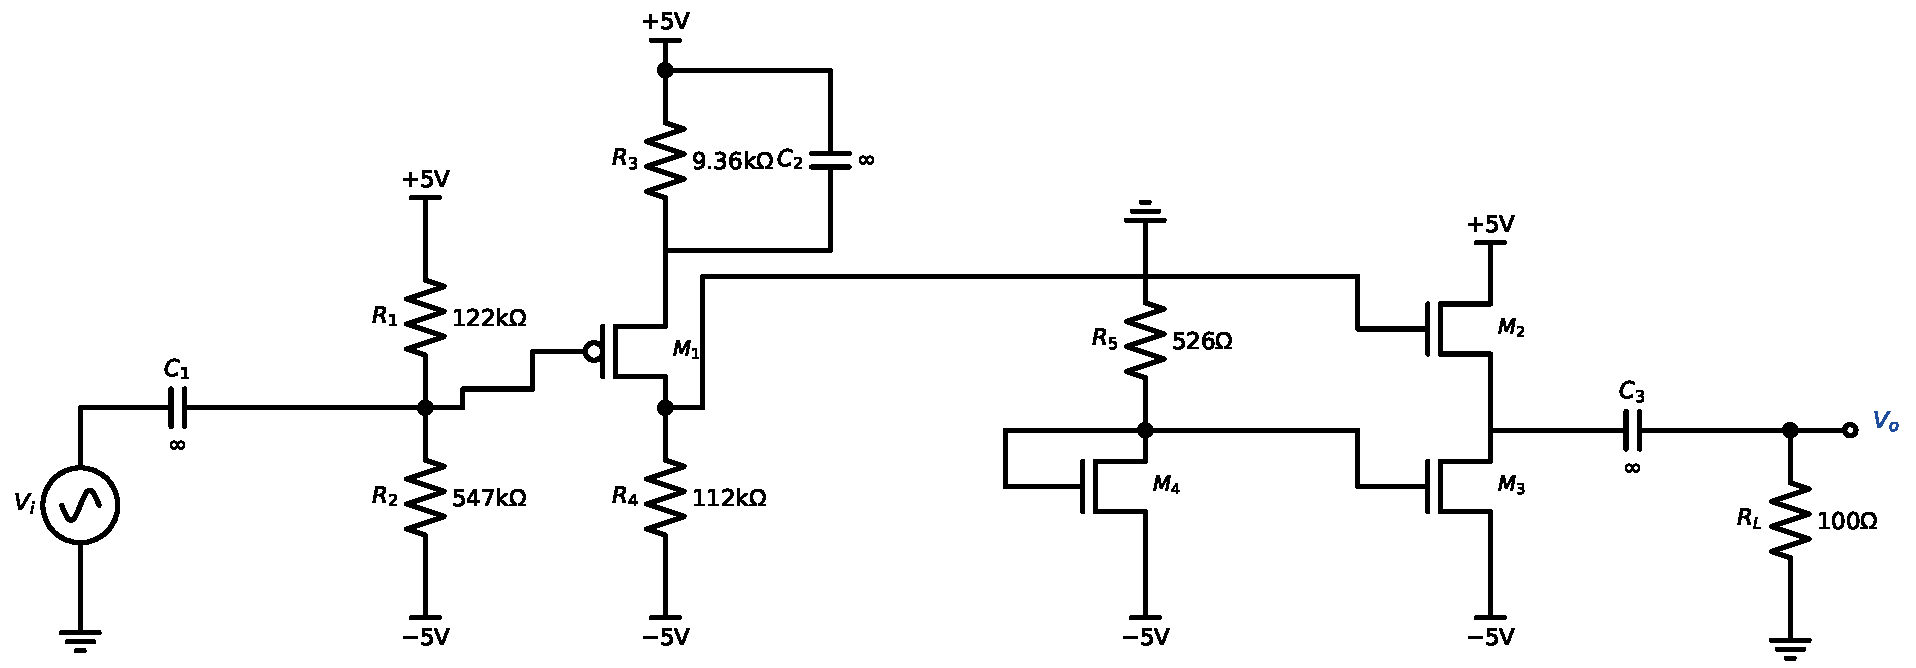
\includegraphics[width=0.85\linewidth,height=6cm,keepaspectratio]{p12_designed}\end{center}

\begin{ansbox}
$R_{1} = 122\,\mathrm{k}\Omega$,\quad $R_{2} = 547\,\mathrm{k}\Omega$,\quad $R_{3} = 9.36\,\mathrm{k}\Omega$,\quad $R_{4} = 112\,\mathrm{k}\Omega$,\quad $R_{5} = 526\,\Omega$
\end{ansbox}

\newpage
\subsection*{Solution 5E.13 \hfill Hard}
\begin{center}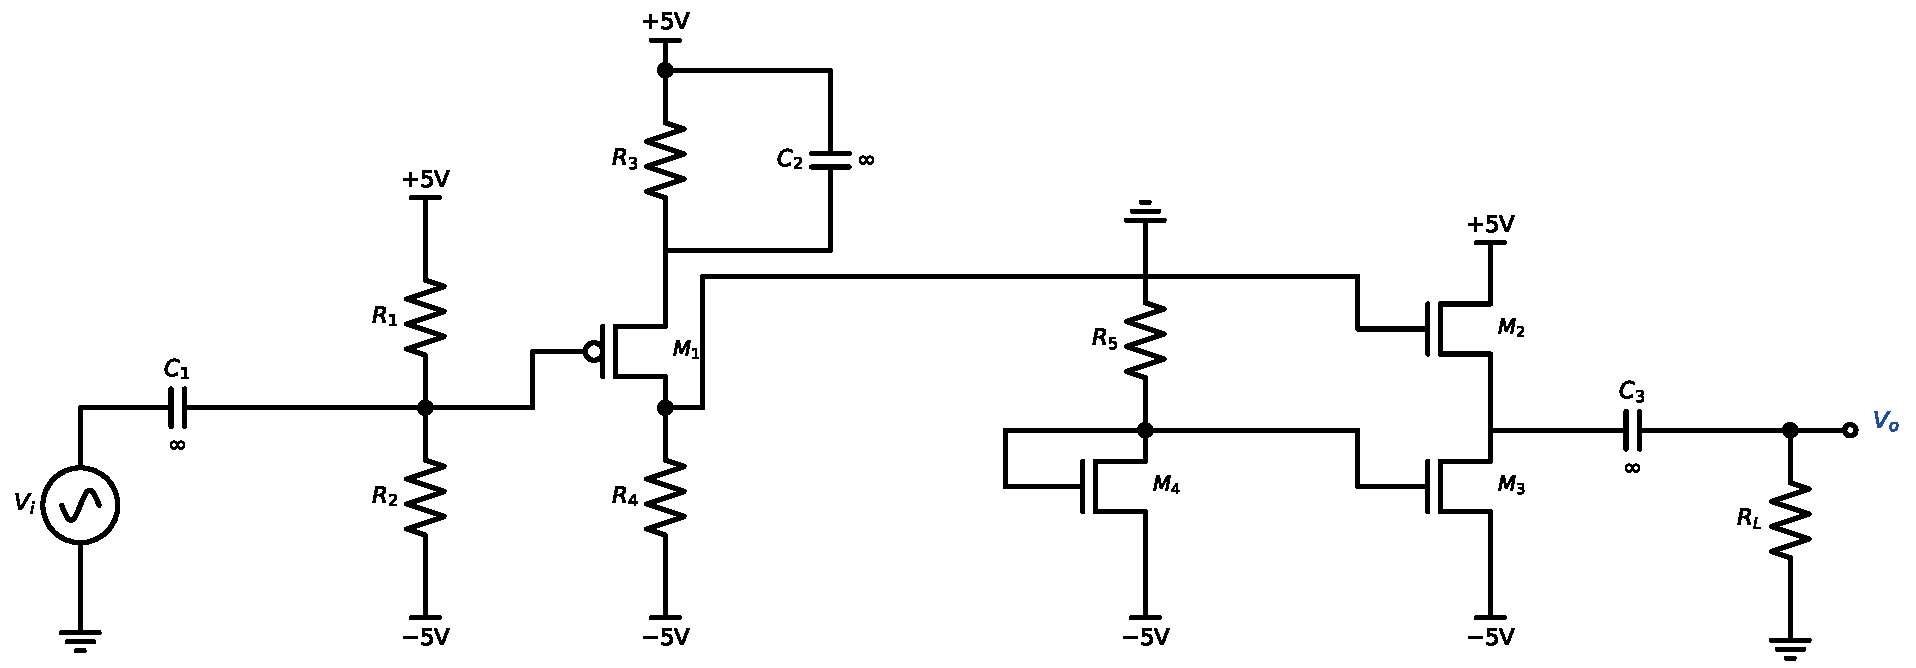
\includegraphics[width=0.9\linewidth,height=6cm,keepaspectratio]{p13_circuit}\end{center}
\solstep{1}{Plan}Follow the procedure of Sample Problem 5: size the output current sink for the load current, then the follower; budget the supply voltage around the drain swing; get $V_{ov1}$ from the gain ($|A_v| = g_mR = 2V_R/V_{ov}$), then the resistors; finally the gate divider from the input resistance. Distortion of a common-source stage: $HD_2 \approx \frac{\hat v_{gs}}{4V_{ov}}$ (from $i_D = \frac{k}{2}(V_{ov} + v_{gs})^2$).
\solstep{2}{Output stage: sink, reference and follower}The sink $M_3$ must deliver the whole peak load current: $I_{D3} \ge \frac{\hat V_o}{R_L} = \frac{2}{100\,\Omega} = 20\,\mathrm{m}\mathrm{A}$; use $I_{D3} = 25\,\mathrm{m}\mathrm{A}$ (given). Then $\frac{k_3}{2}V_{ov3}^2 = I_{D3} \Rightarrow V_{ov3} = \sqrt{\frac{2\cdot25\,\mathrm{m}\mathrm{A}}{50\,\mathrm{m}\mathrm{A/V^2}}} = 1$\,V.

$M_4$ is identical to $M_3$ and has the same $V_{GS}$, so $I_{D4} = I_{D3}$ and $V_{ov4} = V_{ov3}$.

\[R_5 = \frac{5 - |V_{t}| - V_{ov4}}{I_{D4}} = \frac{5 - 2 - 1}{25\,\mathrm{m}\mathrm{A}} = \mathbf{80\,\Omega}\]

The follower $M_2$ carries the same current, $I_{D2} = I_{D3}$, so $V_{ov2} = 1$\,V, $g_{m2} = k_2V_{ov2} = 50\,\mathrm{m}\mathrm{A/V}$, $1/g_{m2} = 20\,\Omega$ and (the sink $M_3$ is a current source, $Z = \infty$) \[A_{v2} = \frac{R_L}{1/g_{m2} + R_L} = \frac{100\,\Omega}{20\,\Omega + 100\,\Omega} = 0.8333\]So the drain of $M_1$ must swing $\hat V_d = \hat V_o/A_{v2} = 2.4$\,V and $|A_{v1}| = |A_v|/A_{v2} = 48$.
\solstep{3}{Common-source stage}Voltage budget of the $V_{DD} + V_{SS} = 10$\,V branch through $R_3$, $M_1$, $R_4$. At the lowest drain voltage of $M_1$ the follower and the sink must both stay active (the drain of $M_1$ sits one $|V_{GS2}|$ away from the output, which needs $V_{ov3}$ of room above the rail): \[V_{R4} \ge V_{ov3} + V_{ov2} + |V_{t2}| + \hat V_d = 1 + 1 + 2 + 2.4 = 6.4\,\mathrm{V}\]$M_1$ must stay active at the other extreme: $V_{R3} + V_{ov1} + \hat V_d + V_{R4} \le 10$, and with $V_{ov1} = 2V_{R4}/|A_{v1}|$ (below): \[V_{R4}\left(1 + \frac{2}{|A_{v1}|}\right) \le 10 - V_{R3} - \hat V_d \Rightarrow V_{R4} \le 6.816\,\mathrm{V}\]$V_{R3} = 0.5$\,V (its minimum) and $V_{R4} = 6.5$\,V (the next multiple of $0.5$\,V above the lower bound).

Gain of the common-source stage ($R_3$ is bypassed, the follower's gate loads nothing): \[|A_{v1}| = g_{m1}R_4 = k_1V_{ov1}\frac{V_{R4}}{\frac{k_1}{2}V_{ov1}^2} = \frac{2V_{R4}}{V_{ov1}} \Rightarrow V_{ov1} = \frac{2\cdot6.5}{48} = 0.2708\,\mathrm{V}\]$I_{D1} = \frac{k_1}{2}V_{ov1}^2 = 36.7\,\mu \mathrm{A}$, $R_4 = \frac{V_{R4}}{I_{D1}} = \mathbf{177\,\mathrm{k}\Omega}$, $R_3 = \frac{V_{R3}}{I_{D1}} = \mathbf{13.6\,\mathrm{k}\Omega}$.

Gate divider: the resistor on the source side of $M_1$ carries $V_{R1} = V_{R3} + |V_{t1}| + V_{ov1} = 1.771$\,V, the other one $V_{R2} = 10 - 1.771 = 8.229$\,V. Both carry the same current ($I_G = 0$): $R_{1} = 1.771X$, $R_{2} = 8.229X$, and the input resistance is their parallel combination: \[R_1\|R_2 = \frac{1.771\cdot8.229}{10}X \ge 50\,\mathrm{k}\Omega \Rightarrow X = 34.3\,\mathrm{k}\Omega:\quad \mathbf{R_1 = 60.8\,\mathrm{k}\Omega},\ \mathbf{R_2 = 282\,\mathrm{k}\Omega}\]
\solstep{4}{Check by analysis}DC analysis of the finished circuit (as in sets 5A/5B):\begin{center}\renewcommand{\arraystretch}{1.35}
\begin{tabular}{cccc}
\toprule
 & $I_D$ & $V_{ov}$ & $|V_{DS}|$ \\
\midrule
$M_{1}$ & $36.7\,\mu \mathrm{A}$ & $0.271$\,V & $3$\,V \\
$M_{4}$ & $25\,\mathrm{m}\mathrm{A}$ & $1$\,V & $3$\,V \\
$M_{2}$ & $25\,\mathrm{m}\mathrm{A}$ & $1$\,V & $6.5$\,V \\
$M_{3}$ & $25\,\mathrm{m}\mathrm{A}$ & $1$\,V & $3.5$\,V \\
\bottomrule
\end{tabular}\end{center}
\begin{itemize}[leftmargin=*,itemsep=2pt]
\item $V_{SD1} = V_{S1} - V_{D1} = 4.5 - 1.5 = 3\,\mathrm{V}$ $\ge V_{ov1} = 0.271$\,V $\Rightarrow$ $M_{1}$ is active \checkmark
\item $M_{4}$ is diode-connected: $V_{DS4} = V_{GS4} > V_{ov4}$, always active \checkmark
\item $V_{DS2} = 5 - V_{S2} = 5 - (-1.5) = 6.5\,\mathrm{V}$ $\ge V_{ov2} = 1$\,V $\Rightarrow$ $M_{2}$ is active \checkmark
\item $V_{DS3} = V_{S2} - (-5) = -1.5 - (-5) = 3.5\,\mathrm{V}$ $\ge V_{ov3} = 1$\,V $\Rightarrow$ $M_{3}$ is active \checkmark
\item Gain (exact small-signal analysis of the finished circuit): $|A_v| = 40$ \checkmark
\item Input resistance $R_1\|R_2 = 50\,\mathrm{k}\Omega \ge 50\,\mathrm{k}\Omega$ \checkmark
\item Output swing before clipping: $M_1$ leaves saturation at $\hat V_o = 2.27$\,V; $M_3$ leaves saturation at $\hat V_o = 2.5$\,V; $M_2$ leaves saturation at $\hat V_o = 5.5$\,V; $M_3$ cannot sink more current (current clipping) at $\hat V_o = 2.5$\,V. The smallest is $2.27$\,V $\ge 2$\,V \checkmark
\item THD $\approx HD_2 = \frac{\hat v_{gs1}}{4V_{ov1}} = \frac{2/40}{4\cdot0.271} = 4.6\,\%$ $\le 10\,\%$ \checkmark
\end{itemize}

\begin{center}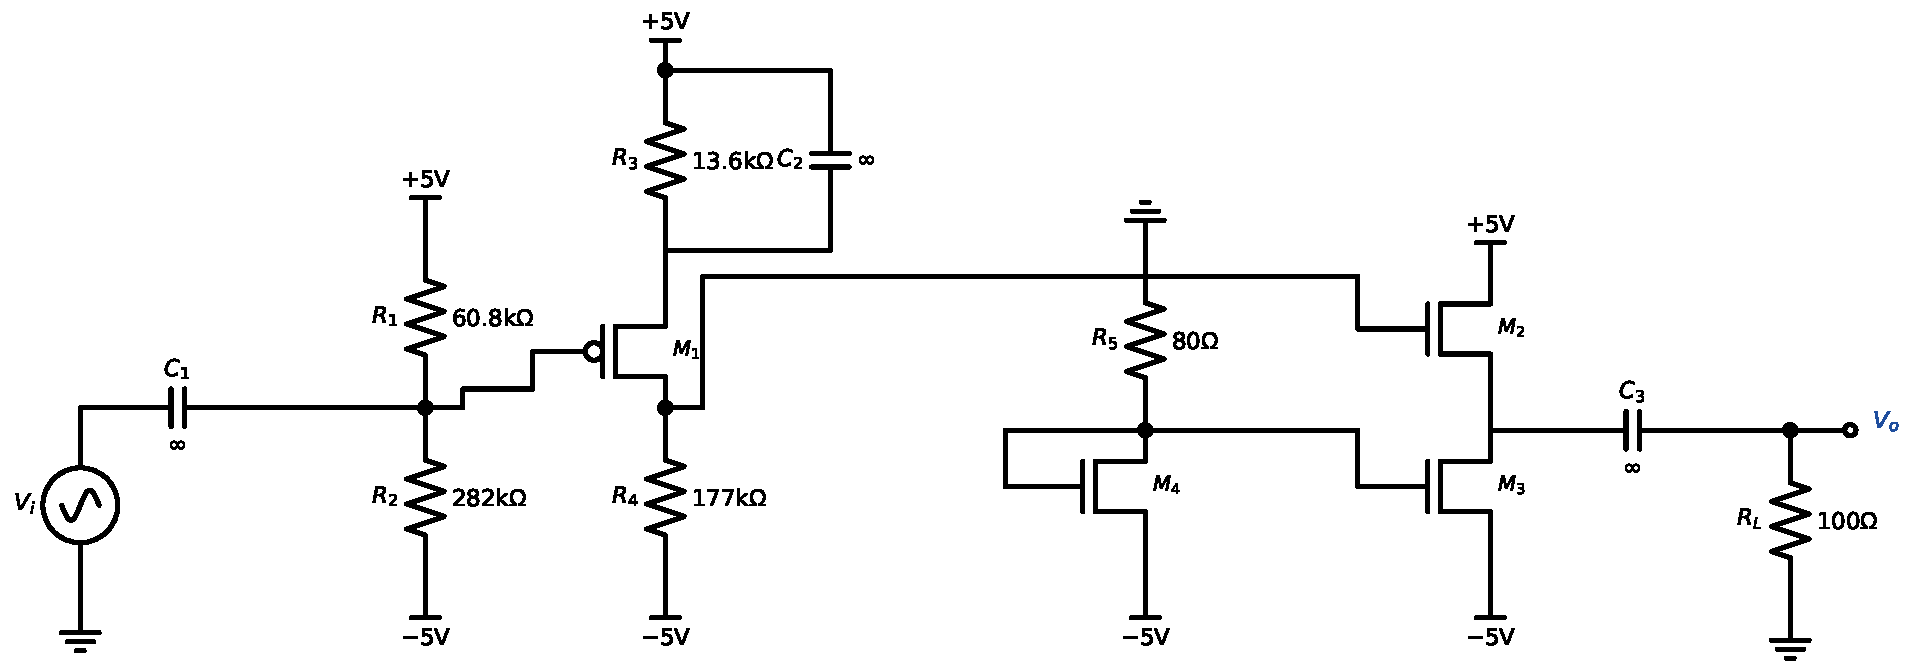
\includegraphics[width=0.85\linewidth,height=6cm,keepaspectratio]{p13_designed}\end{center}

\begin{ansbox}
$R_{1} = 60.8\,\mathrm{k}\Omega$,\quad $R_{2} = 282\,\mathrm{k}\Omega$,\quad $R_{3} = 13.6\,\mathrm{k}\Omega$,\quad $R_{4} = 177\,\mathrm{k}\Omega$,\quad $R_{5} = 80\,\Omega$
\end{ansbox}

\newpage
\subsection*{Solution 5E.14 \hfill Hard}
\begin{center}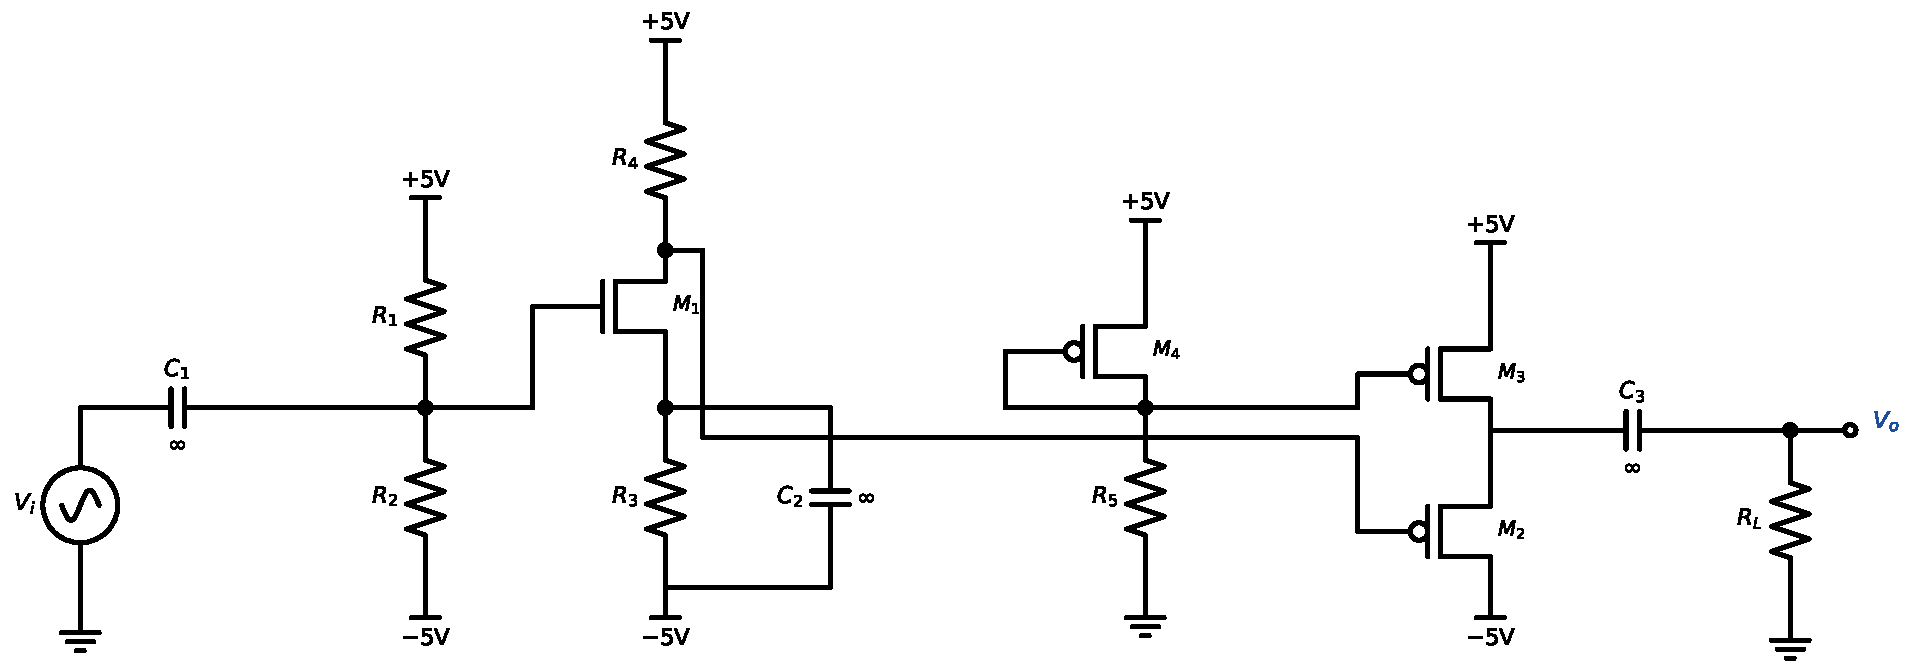
\includegraphics[width=0.9\linewidth,height=6cm,keepaspectratio]{p14_circuit}\end{center}
\solstep{1}{Plan}Follow the procedure of Sample Problem 5: size the output current sink for the load current, then the follower; budget the supply voltage around the drain swing; get $V_{ov1}$ from the gain ($|A_v| = g_mR = 2V_R/V_{ov}$), then the resistors; finally the gate divider from the input resistance. Distortion of a common-source stage: $HD_2 \approx \frac{\hat v_{gs}}{4V_{ov}}$ (from $i_D = \frac{k}{2}(V_{ov} + v_{gs})^2$).
\solstep{2}{Output stage: sink, reference and follower}The sink $M_3$ must deliver the whole peak load current: $I_{D3} \ge \frac{\hat V_o}{R_L} = \frac{2}{100\,\Omega} = 20\,\mathrm{m}\mathrm{A}$; use $I_{D3} = 25\,\mathrm{m}\mathrm{A}$ (given). Then $\frac{k_3}{2}V_{ov3}^2 = I_{D3} \Rightarrow V_{ov3} = \sqrt{\frac{2\cdot25\,\mathrm{m}\mathrm{A}}{50\,\mathrm{m}\mathrm{A/V^2}}} = 1$\,V.

$M_4$ is identical to $M_3$ and has the same $V_{GS}$, so $I_{D4} = I_{D3}$ and $V_{ov4} = V_{ov3}$.

\[R_5 = \frac{5 - |V_{t}| - V_{ov4}}{I_{D4}} = \frac{5 - 2 - 1}{25\,\mathrm{m}\mathrm{A}} = \mathbf{80\,\Omega}\]

The follower $M_2$ carries the same current, $I_{D2} = I_{D3}$, so $V_{ov2} = 1$\,V, $g_{m2} = k_2V_{ov2} = 50\,\mathrm{m}\mathrm{A/V}$, $1/g_{m2} = 20\,\Omega$ and (the sink $M_3$ is a current source, $Z = \infty$) \[A_{v2} = \frac{R_L}{1/g_{m2} + R_L} = \frac{100\,\Omega}{20\,\Omega + 100\,\Omega} = 0.8333\]So the drain of $M_1$ must swing $\hat V_d = \hat V_o/A_{v2} = 2.4$\,V and $|A_{v1}| = |A_v|/A_{v2} = 48$.
\solstep{3}{Common-source stage}Voltage budget of the $V_{DD} + V_{SS} = 10$\,V branch through $R_3$, $M_1$, $R_4$. At the highest drain voltage of $M_1$ the follower and the sink must both stay active (the drain of $M_1$ sits one $|V_{GS2}|$ away from the output, which needs $V_{ov3}$ of room above the rail): \[V_{R4} \ge V_{ov3} + V_{ov2} + |V_{t2}| + \hat V_d = 1 + 1 + 2 + 2.4 = 6.4\,\mathrm{V}\]$M_1$ must stay active at the other extreme: $V_{R3} + V_{ov1} + \hat V_d + V_{R4} \le 10$, and with $V_{ov1} = 2V_{R4}/|A_{v1}|$ (below): \[V_{R4}\left(1 + \frac{2}{|A_{v1}|}\right) \le 10 - V_{R3} - \hat V_d \Rightarrow V_{R4} \le 6.816\,\mathrm{V}\]$V_{R3} = 0.5$\,V (its minimum) and $V_{R4} = 6.5$\,V (the next multiple of $0.5$\,V above the lower bound).

Gain of the common-source stage ($R_3$ is bypassed, the follower's gate loads nothing): \[|A_{v1}| = g_{m1}R_4 = k_1V_{ov1}\frac{V_{R4}}{\frac{k_1}{2}V_{ov1}^2} = \frac{2V_{R4}}{V_{ov1}} \Rightarrow V_{ov1} = \frac{2\cdot6.5}{48} = 0.2708\,\mathrm{V}\]$I_{D1} = \frac{k_1}{2}V_{ov1}^2 = 36.7\,\mu \mathrm{A}$, $R_4 = \frac{V_{R4}}{I_{D1}} = \mathbf{177\,\mathrm{k}\Omega}$, $R_3 = \frac{V_{R3}}{I_{D1}} = \mathbf{13.6\,\mathrm{k}\Omega}$.

Gate divider: the resistor on the source side of $M_1$ carries $V_{R2} = V_{R3} + |V_{t1}| + V_{ov1} = 1.771$\,V, the other one $V_{R1} = 10 - 1.771 = 8.229$\,V. Both carry the same current ($I_G = 0$): $R_{2} = 1.771X$, $R_{1} = 8.229X$, and the input resistance is their parallel combination: \[R_1\|R_2 = \frac{1.771\cdot8.229}{10}X \ge 50\,\mathrm{k}\Omega \Rightarrow X = 34.3\,\mathrm{k}\Omega:\quad \mathbf{R_1 = 282\,\mathrm{k}\Omega},\ \mathbf{R_2 = 60.8\,\mathrm{k}\Omega}\]
\solstep{4}{Check by analysis}DC analysis of the finished circuit (as in sets 5A/5B):\begin{center}\renewcommand{\arraystretch}{1.35}
\begin{tabular}{cccc}
\toprule
 & $I_D$ & $V_{ov}$ & $|V_{DS}|$ \\
\midrule
$M_{1}$ & $36.7\,\mu \mathrm{A}$ & $0.271$\,V & $3$\,V \\
$M_{4}$ & $25\,\mathrm{m}\mathrm{A}$ & $1$\,V & $3$\,V \\
$M_{3}$ & $25\,\mathrm{m}\mathrm{A}$ & $1$\,V & $3.5$\,V \\
$M_{2}$ & $25\,\mathrm{m}\mathrm{A}$ & $1$\,V & $6.5$\,V \\
\bottomrule
\end{tabular}\end{center}
\begin{itemize}[leftmargin=*,itemsep=2pt]
\item $V_{DS1} = V_{D1} - V_{S1} = -1.5 - (-4.5) = 3\,\mathrm{V}$ $\ge V_{ov1} = 0.271$\,V $\Rightarrow$ $M_{1}$ is active \checkmark
\item $M_{4}$ is diode-connected: $V_{SD4} = V_{SG4} > V_{ov4}$, always active \checkmark
\item $V_{SD3} = 5 - V_{D3} = 5 - 1.5 = 3.5\,\mathrm{V}$ $\ge V_{ov3} = 1$\,V $\Rightarrow$ $M_{3}$ is active \checkmark
\item $V_{SD2} = V_{D3} - (-5) = 1.5 - (-5) = 6.5\,\mathrm{V}$ $\ge V_{ov2} = 1$\,V $\Rightarrow$ $M_{2}$ is active \checkmark
\item Gain (exact small-signal analysis of the finished circuit): $|A_v| = 40$ \checkmark
\item Input resistance $R_1\|R_2 = 50\,\mathrm{k}\Omega \ge 50\,\mathrm{k}\Omega$ \checkmark
\item Output swing before clipping: $M_1$ leaves saturation at $\hat V_o = 2.27$\,V; $M_3$ leaves saturation at $\hat V_o = 2.5$\,V; $M_2$ leaves saturation at $\hat V_o = 5.5$\,V; $M_3$ cannot sink more current (current clipping) at $\hat V_o = 2.5$\,V. The smallest is $2.27$\,V $\ge 2$\,V \checkmark
\item THD $\approx HD_2 = \frac{\hat v_{gs1}}{4V_{ov1}} = \frac{2/40}{4\cdot0.271} = 4.6\,\%$ $\le 10\,\%$ \checkmark
\end{itemize}

\begin{center}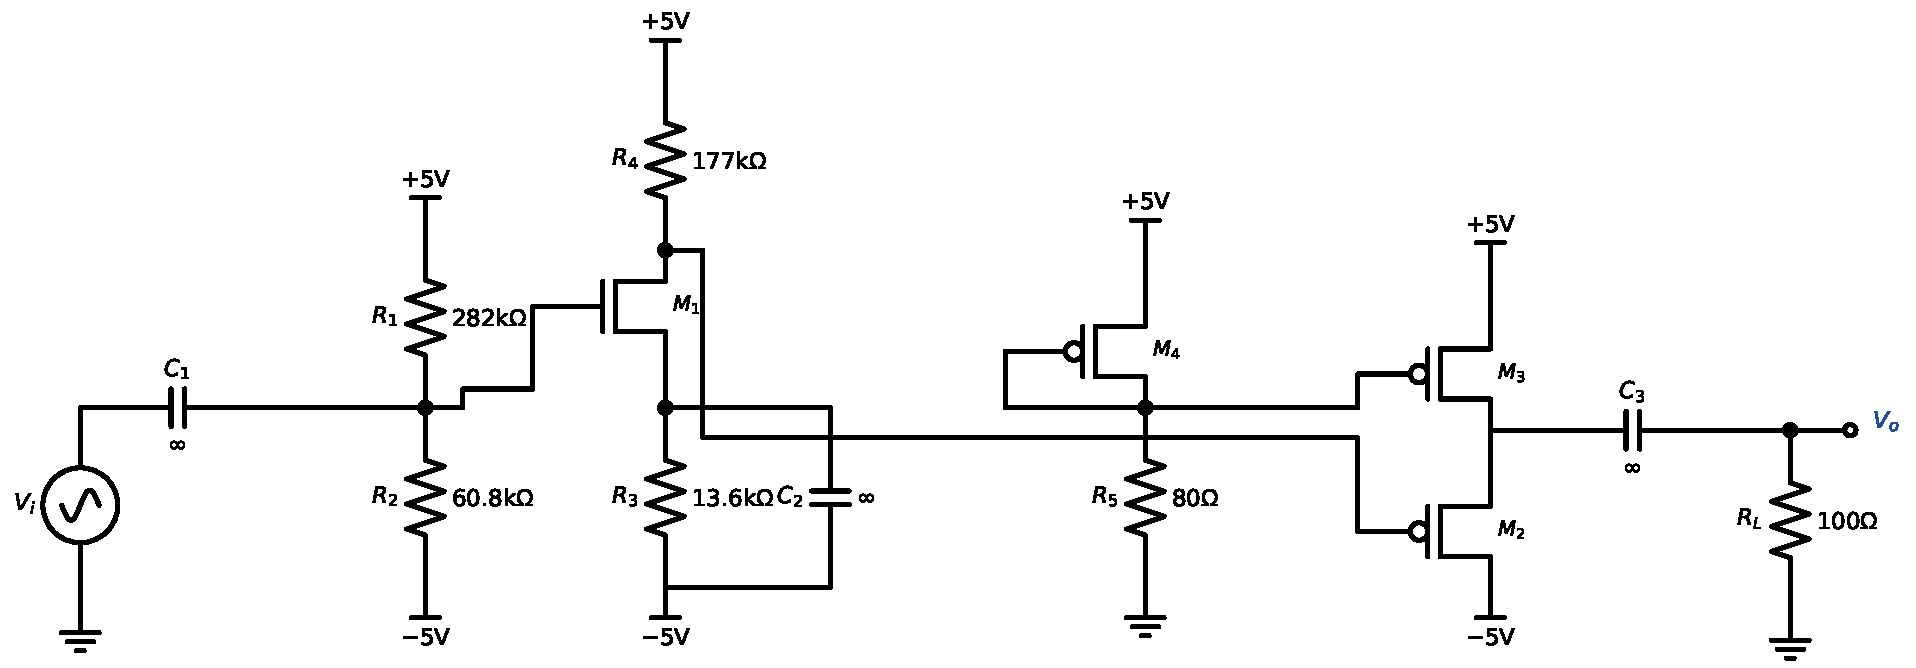
\includegraphics[width=0.85\linewidth,height=6cm,keepaspectratio]{p14_designed}\end{center}

\begin{ansbox}
$R_{1} = 282\,\mathrm{k}\Omega$,\quad $R_{2} = 60.8\,\mathrm{k}\Omega$,\quad $R_{3} = 13.6\,\mathrm{k}\Omega$,\quad $R_{4} = 177\,\mathrm{k}\Omega$,\quad $R_{5} = 80\,\Omega$
\end{ansbox}

\newpage
\subsection*{Solution 5E.15 \hfill Hard}
\begin{center}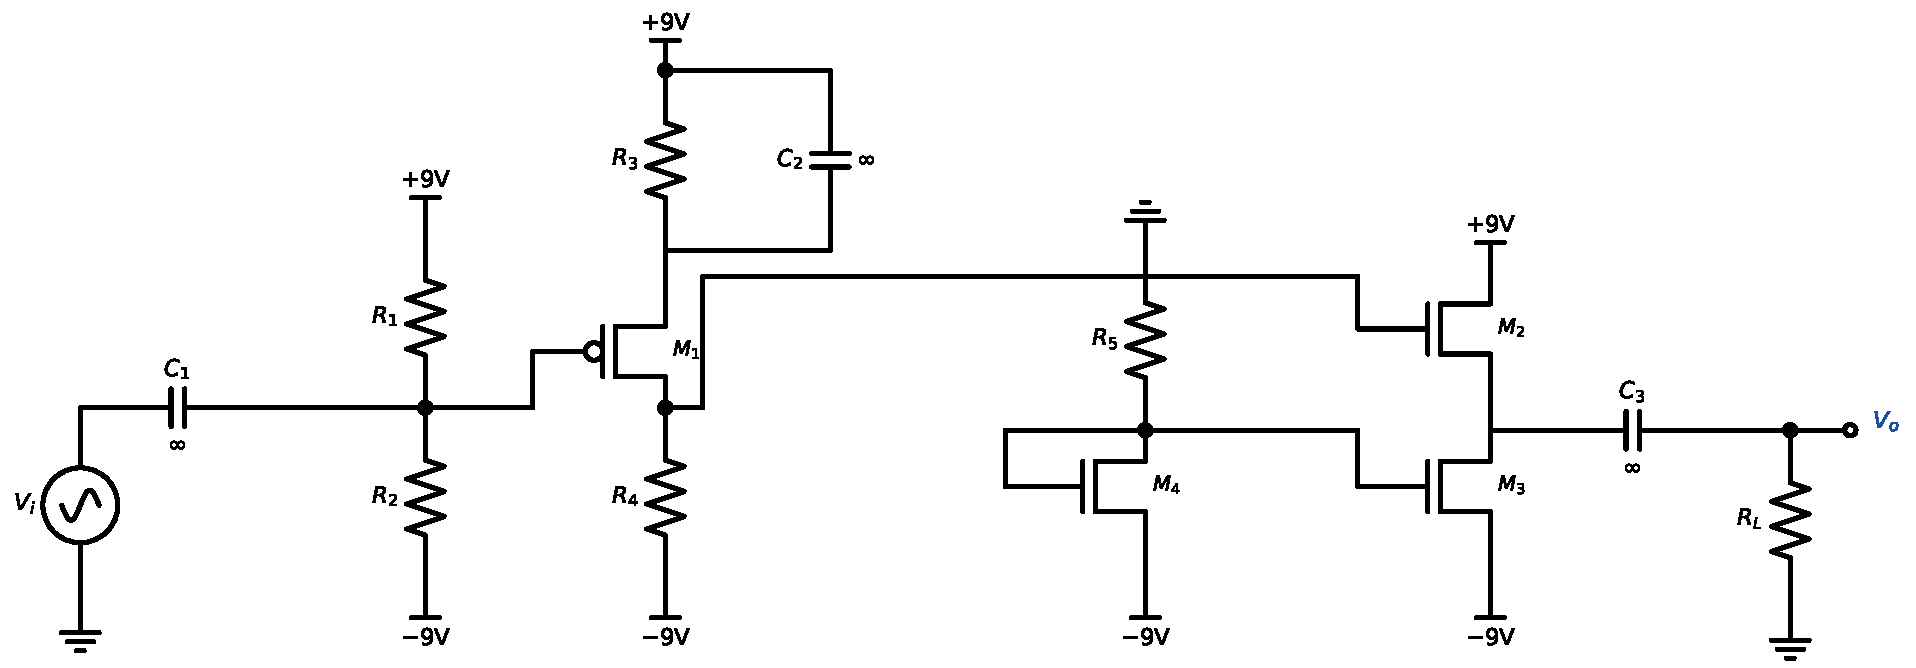
\includegraphics[width=0.9\linewidth,height=6cm,keepaspectratio]{p15_circuit}\end{center}
\solstep{1}{Plan}Follow the procedure of Sample Problem 5: size the output current sink for the load current, then the follower; budget the supply voltage around the drain swing; get $V_{ov1}$ from the gain ($|A_v| = g_mR = 2V_R/V_{ov}$), then the resistors; finally the gate divider from the input resistance. Distortion of a common-source stage: $HD_2 \approx \frac{\hat v_{gs}}{4V_{ov}}$ (from $i_D = \frac{k}{2}(V_{ov} + v_{gs})^2$).
\solstep{2}{Output stage: sink, reference and follower}The sink $M_3$ must deliver the whole peak load current: $I_{D3} \ge \frac{\hat V_o}{R_L} = \frac{4}{100\,\Omega} = 40\,\mathrm{m}\mathrm{A}$; use $I_{D3} = 45\,\mathrm{m}\mathrm{A}$ (given). Then $\frac{k_3}{2}V_{ov3}^2 = I_{D3} \Rightarrow V_{ov3} = \sqrt{\frac{2\cdot45\,\mathrm{m}\mathrm{A}}{50\,\mathrm{m}\mathrm{A/V^2}}} = 1.342$\,V.

$M_4$ is identical to $M_3$ and has the same $V_{GS}$, so $I_{D4} = I_{D3}$ and $V_{ov4} = V_{ov3}$.

\[R_5 = \frac{9 - |V_{t}| - V_{ov4}}{I_{D4}} = \frac{9 - 2 - 1.342}{45\,\mathrm{m}\mathrm{A}} = \mathbf{126\,\Omega}\]

The follower $M_2$ carries the same current, $I_{D2} = I_{D3}$, so $V_{ov2} = 1.342$\,V, $g_{m2} = k_2V_{ov2} = 67.1\,\mathrm{m}\mathrm{A/V}$, $1/g_{m2} = 14.9\,\Omega$ and (the sink $M_3$ is a current source, $Z = \infty$) \[A_{v2} = \frac{R_L}{1/g_{m2} + R_L} = \frac{100\,\Omega}{14.9\,\Omega + 100\,\Omega} = 0.8703\]So the drain of $M_1$ must swing $\hat V_d = \hat V_o/A_{v2} = 4.596$\,V and $|A_{v1}| = |A_v|/A_{v2} = 57.45$.
\solstep{3}{Common-source stage}Voltage budget of the $V_{DD} + V_{SS} = 18$\,V branch through $R_3$, $M_1$, $R_4$. At the lowest drain voltage of $M_1$ the follower and the sink must both stay active (the drain of $M_1$ sits one $|V_{GS2}|$ away from the output, which needs $V_{ov3}$ of room above the rail): \[V_{R4} \ge V_{ov3} + V_{ov2} + |V_{t2}| + \hat V_d = 1.34 + 1.34 + 2 + 4.6 = 9.28\,\mathrm{V}\]$M_1$ must stay active at the other extreme: $V_{R3} + V_{ov1} + \hat V_d + V_{R4} \le 18$, and with $V_{ov1} = 2V_{R4}/|A_{v1}|$ (below): \[V_{R4}\left(1 + \frac{2}{|A_{v1}|}\right) \le 18 - V_{R3} - \hat V_d \Rightarrow V_{R4} \le 11.99\,\mathrm{V}\]$V_{R3} = 1$\,V (its minimum) and $V_{R4} = 9.5$\,V (the next multiple of $0.5$\,V above the lower bound).

Gain of the common-source stage ($R_3$ is bypassed, the follower's gate loads nothing): \[|A_{v1}| = g_{m1}R_4 = k_1V_{ov1}\frac{V_{R4}}{\frac{k_1}{2}V_{ov1}^2} = \frac{2V_{R4}}{V_{ov1}} \Rightarrow V_{ov1} = \frac{2\cdot9.5}{57.45} = 0.3307\,\mathrm{V}\]$I_{D1} = \frac{k_1}{2}V_{ov1}^2 = 54.7\,\mu \mathrm{A}$, $R_4 = \frac{V_{R4}}{I_{D1}} = \mathbf{174\,\mathrm{k}\Omega}$, $R_3 = \frac{V_{R3}}{I_{D1}} = \mathbf{18.3\,\mathrm{k}\Omega}$.

Gate divider: the resistor on the source side of $M_1$ carries $V_{R1} = V_{R3} + |V_{t1}| + V_{ov1} = 2.331$\,V, the other one $V_{R2} = 18 - 2.331 = 15.67$\,V. Both carry the same current ($I_G = 0$): $R_{1} = 2.331X$, $R_{2} = 15.67X$, and the input resistance is their parallel combination: \[R_1\|R_2 = \frac{2.331\cdot15.67}{18}X \ge 100\,\mathrm{k}\Omega \Rightarrow X = 49.3\,\mathrm{k}\Omega:\quad \mathbf{R_1 = 115\,\mathrm{k}\Omega},\ \mathbf{R_2 = 772\,\mathrm{k}\Omega}\]
\solstep{4}{Check by analysis}DC analysis of the finished circuit (as in sets 5A/5B):\begin{center}\renewcommand{\arraystretch}{1.35}
\begin{tabular}{cccc}
\toprule
 & $I_D$ & $V_{ov}$ & $|V_{DS}|$ \\
\midrule
$M_{1}$ & $54.7\,\mu \mathrm{A}$ & $0.331$\,V & $7.5$\,V \\
$M_{4}$ & $45\,\mathrm{m}\mathrm{A}$ & $1.34$\,V & $3.342$\,V \\
$M_{2}$ & $45\,\mathrm{m}\mathrm{A}$ & $1.34$\,V & $11.84$\,V \\
$M_{3}$ & $45\,\mathrm{m}\mathrm{A}$ & $1.34$\,V & $6.158$\,V \\
\bottomrule
\end{tabular}\end{center}
\begin{itemize}[leftmargin=*,itemsep=2pt]
\item $V_{SD1} = V_{S1} - V_{D1} = 8 - 0.5 = 7.5\,\mathrm{V}$ $\ge V_{ov1} = 0.331$\,V $\Rightarrow$ $M_{1}$ is active \checkmark
\item $M_{4}$ is diode-connected: $V_{DS4} = V_{GS4} > V_{ov4}$, always active \checkmark
\item $V_{DS2} = 9 - V_{S2} = 9 - (-2.842) = 11.8\,\mathrm{V}$ $\ge V_{ov2} = 1.34$\,V $\Rightarrow$ $M_{2}$ is active \checkmark
\item $V_{DS3} = V_{S2} - (-9) = -2.842 - (-9) = 6.16\,\mathrm{V}$ $\ge V_{ov3} = 1.34$\,V $\Rightarrow$ $M_{3}$ is active \checkmark
\item Gain (exact small-signal analysis of the finished circuit): $|A_v| = 50$ \checkmark
\item Input resistance $R_1\|R_2 = 100\,\mathrm{k}\Omega \ge 100\,\mathrm{k}\Omega$ \checkmark
\item Output swing before clipping: $M_1$ leaves saturation at $\hat V_o = 6.24$\,V; $M_3$ leaves saturation at $\hat V_o = 4.82$\,V; $M_2$ leaves saturation at $\hat V_o = 10.5$\,V; $M_3$ cannot sink more current (current clipping) at $\hat V_o = 4.5$\,V. The smallest is $4.5$\,V $\ge 4$\,V \checkmark
\item THD $\approx HD_2 = \frac{\hat v_{gs1}}{4V_{ov1}} = \frac{4/50}{4\cdot0.331} = 6\,\%$ $\le 10\,\%$ \checkmark
\end{itemize}

\begin{center}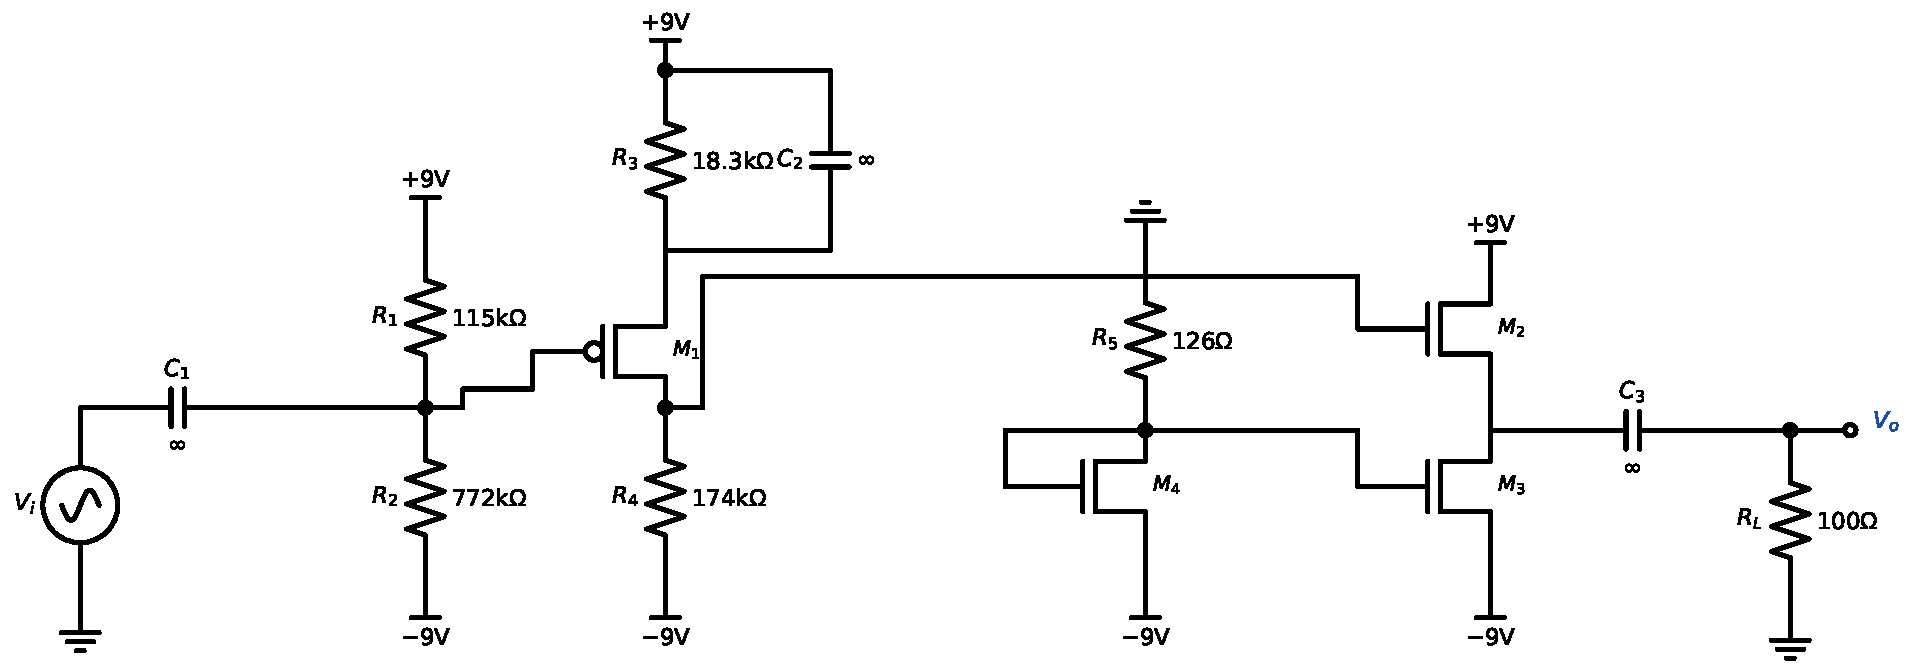
\includegraphics[width=0.85\linewidth,height=6cm,keepaspectratio]{p15_designed}\end{center}

\begin{ansbox}
$R_{1} = 115\,\mathrm{k}\Omega$,\quad $R_{2} = 772\,\mathrm{k}\Omega$,\quad $R_{3} = 18.3\,\mathrm{k}\Omega$,\quad $R_{4} = 174\,\mathrm{k}\Omega$,\quad $R_{5} = 126\,\Omega$
\end{ansbox}

\newpage
\subsection*{Solution 5E.16 \hfill Hard}
\begin{center}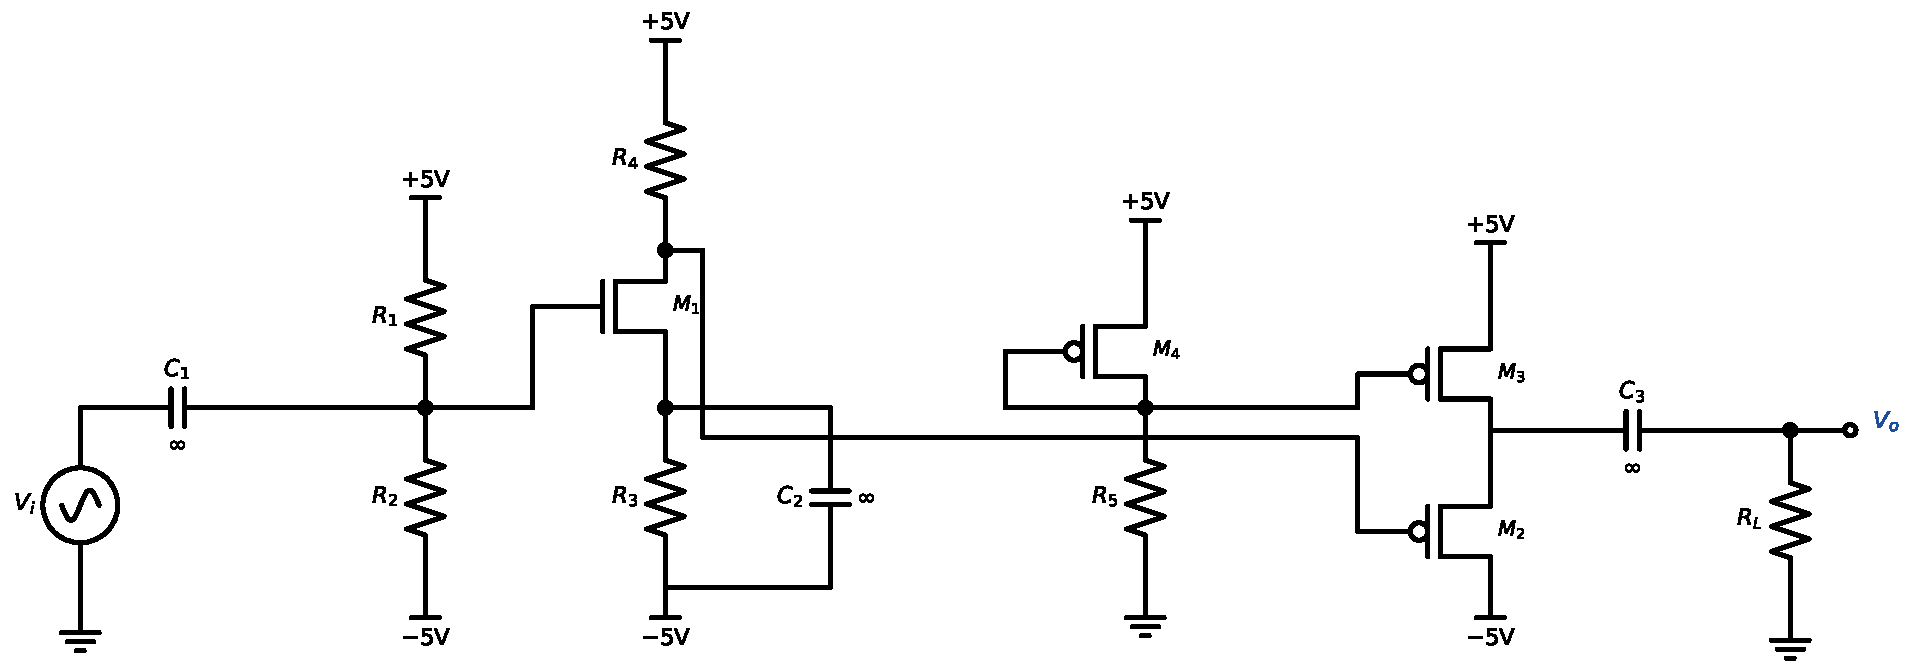
\includegraphics[width=0.9\linewidth,height=6cm,keepaspectratio]{p16_circuit}\end{center}
\solstep{1}{Plan}Follow the procedure of Sample Problem 5: size the output current sink for the load current, then the follower; budget the supply voltage around the drain swing; get $V_{ov1}$ from the gain ($|A_v| = g_mR = 2V_R/V_{ov}$), then the resistors; finally the gate divider from the input resistance. Distortion of a common-source stage: $HD_2 \approx \frac{\hat v_{gs}}{4V_{ov}}$ (from $i_D = \frac{k}{2}(V_{ov} + v_{gs})^2$).
\solstep{2}{Output stage: sink, reference and follower}The sink $M_3$ must deliver the whole peak load current: $I_{D3} \ge \frac{\hat V_o}{R_L} = \frac{1.5}{50\,\Omega} = 30\,\mathrm{m}\mathrm{A}$; use $I_{D3} = 35\,\mathrm{m}\mathrm{A}$ (given). Then $\frac{k_3}{2}V_{ov3}^2 = I_{D3} \Rightarrow V_{ov3} = \sqrt{\frac{2\cdot35\,\mathrm{m}\mathrm{A}}{60\,\mathrm{m}\mathrm{A/V^2}}} = 1.08$\,V.

$M_4$ has the same $V_{GS}$ as $M_3$ but $k_4 = 0.25\,k_3$, so $I_{D4} = 0.25\,I_{D3} = 8.75\,\mathrm{m}\mathrm{A}$ (same $V_{ov}$).

\[R_5 = \frac{5 - |V_{t}| - V_{ov4}}{I_{D4}} = \frac{5 - 1.2 - 1.08}{8.75\,\mathrm{m}\mathrm{A}} = \mathbf{311\,\Omega}\]

The follower $M_2$ carries the same current, $I_{D2} = I_{D3}$, so $V_{ov2} = 1.08$\,V, $g_{m2} = k_2V_{ov2} = 64.8\,\mathrm{m}\mathrm{A/V}$, $1/g_{m2} = 15.4\,\Omega$ and (the sink $M_3$ is a current source, $Z = \infty$) \[A_{v2} = \frac{R_L}{1/g_{m2} + R_L} = \frac{50\,\Omega}{15.4\,\Omega + 50\,\Omega} = 0.7642\]So the drain of $M_1$ must swing $\hat V_d = \hat V_o/A_{v2} = 1.963$\,V and $|A_{v1}| = |A_v|/A_{v2} = 39.26$.
\solstep{3}{Common-source stage}Voltage budget of the $V_{DD} + V_{SS} = 10$\,V branch through $R_3$, $M_1$, $R_4$. At the highest drain voltage of $M_1$ the follower and the sink must both stay active (the drain of $M_1$ sits one $|V_{GS2}|$ away from the output, which needs $V_{ov3}$ of room above the rail): \[V_{R4} \ge V_{ov3} + V_{ov2} + |V_{t2}| + \hat V_d = 1.08 + 1.08 + 1.2 + 1.96 = 5.323\,\mathrm{V}\]$M_1$ must stay active at the other extreme: $V_{R3} + V_{ov1} + \hat V_d + V_{R4} \le 10$, and with $V_{ov1} = 2V_{R4}/|A_{v1}|$ (below): \[V_{R4}\left(1 + \frac{2}{|A_{v1}|}\right) \le 10 - V_{R3} - \hat V_d \Rightarrow V_{R4} \le 7.172\,\mathrm{V}\]$V_{R3} = 0.5$\,V (its minimum) and $V_{R4} = 5.5$\,V (the next multiple of $0.5$\,V above the lower bound).

Gain of the common-source stage ($R_3$ is bypassed, the follower's gate loads nothing): \[|A_{v1}| = g_{m1}R_4 = k_1V_{ov1}\frac{V_{R4}}{\frac{k_1}{2}V_{ov1}^2} = \frac{2V_{R4}}{V_{ov1}} \Rightarrow V_{ov1} = \frac{2\cdot5.5}{39.26} = 0.2802\,\mathrm{V}\]$I_{D1} = \frac{k_1}{2}V_{ov1}^2 = 78.5\,\mu \mathrm{A}$, $R_4 = \frac{V_{R4}}{I_{D1}} = \mathbf{70.1\,\mathrm{k}\Omega}$, $R_3 = \frac{V_{R3}}{I_{D1}} = \mathbf{6.37\,\mathrm{k}\Omega}$.

Gate divider: the resistor on the source side of $M_1$ carries $V_{R2} = V_{R3} + |V_{t1}| + V_{ov1} = 1.58$\,V, the other one $V_{R1} = 10 - 1.58 = 8.42$\,V. Both carry the same current ($I_G = 0$): $R_{2} = 1.58X$, $R_{1} = 8.42X$, and the input resistance is their parallel combination: \[R_1\|R_2 = \frac{1.58\cdot8.42}{10}X \ge 200\,\mathrm{k}\Omega \Rightarrow X = 150\,\mathrm{k}\Omega:\quad \mathbf{R_1 = 1.27\,\mathrm{M}\Omega},\ \mathbf{R_2 = 238\,\mathrm{k}\Omega}\]
\solstep{4}{Check by analysis}DC analysis of the finished circuit (as in sets 5A/5B):\begin{center}\renewcommand{\arraystretch}{1.35}
\begin{tabular}{cccc}
\toprule
 & $I_D$ & $V_{ov}$ & $|V_{DS}|$ \\
\midrule
$M_{1}$ & $78.5\,\mu \mathrm{A}$ & $0.28$\,V & $4$\,V \\
$M_{4}$ & $8.75\,\mathrm{m}\mathrm{A}$ & $1.08$\,V & $2.28$\,V \\
$M_{3}$ & $35\,\mathrm{m}\mathrm{A}$ & $1.08$\,V & $3.22$\,V \\
$M_{2}$ & $35\,\mathrm{m}\mathrm{A}$ & $1.08$\,V & $6.78$\,V \\
\bottomrule
\end{tabular}\end{center}
\begin{itemize}[leftmargin=*,itemsep=2pt]
\item $V_{DS1} = V_{D1} - V_{S1} = -0.5 - (-4.5) = 4\,\mathrm{V}$ $\ge V_{ov1} = 0.28$\,V $\Rightarrow$ $M_{1}$ is active \checkmark
\item $M_{4}$ is diode-connected: $V_{SD4} = V_{SG4} > V_{ov4}$, always active \checkmark
\item $V_{SD3} = 5 - V_{D3} = 5 - 1.78 = 3.22\,\mathrm{V}$ $\ge V_{ov3} = 1.08$\,V $\Rightarrow$ $M_{3}$ is active \checkmark
\item $V_{SD2} = V_{D3} - (-5) = 1.78 - (-5) = 6.78\,\mathrm{V}$ $\ge V_{ov2} = 1.08$\,V $\Rightarrow$ $M_{2}$ is active \checkmark
\item Gain (exact small-signal analysis of the finished circuit): $|A_v| = 30$ \checkmark
\item Input resistance $R_1\|R_2 = 200\,\mathrm{k}\Omega \ge 200\,\mathrm{k}\Omega$ \checkmark
\item Output swing before clipping: $M_1$ leaves saturation at $\hat V_o = 2.84$\,V; $M_3$ leaves saturation at $\hat V_o = 2.14$\,V; $M_2$ leaves saturation at $\hat V_o = 5.7$\,V; $M_3$ cannot sink more current (current clipping) at $\hat V_o = 1.75$\,V. The smallest is $1.75$\,V $\ge 1.5$\,V \checkmark
\item THD $\approx HD_2 = \frac{\hat v_{gs1}}{4V_{ov1}} = \frac{1.5/30}{4\cdot0.28} = 4.5\,\%$ $\le 8\,\%$ \checkmark
\end{itemize}

\begin{center}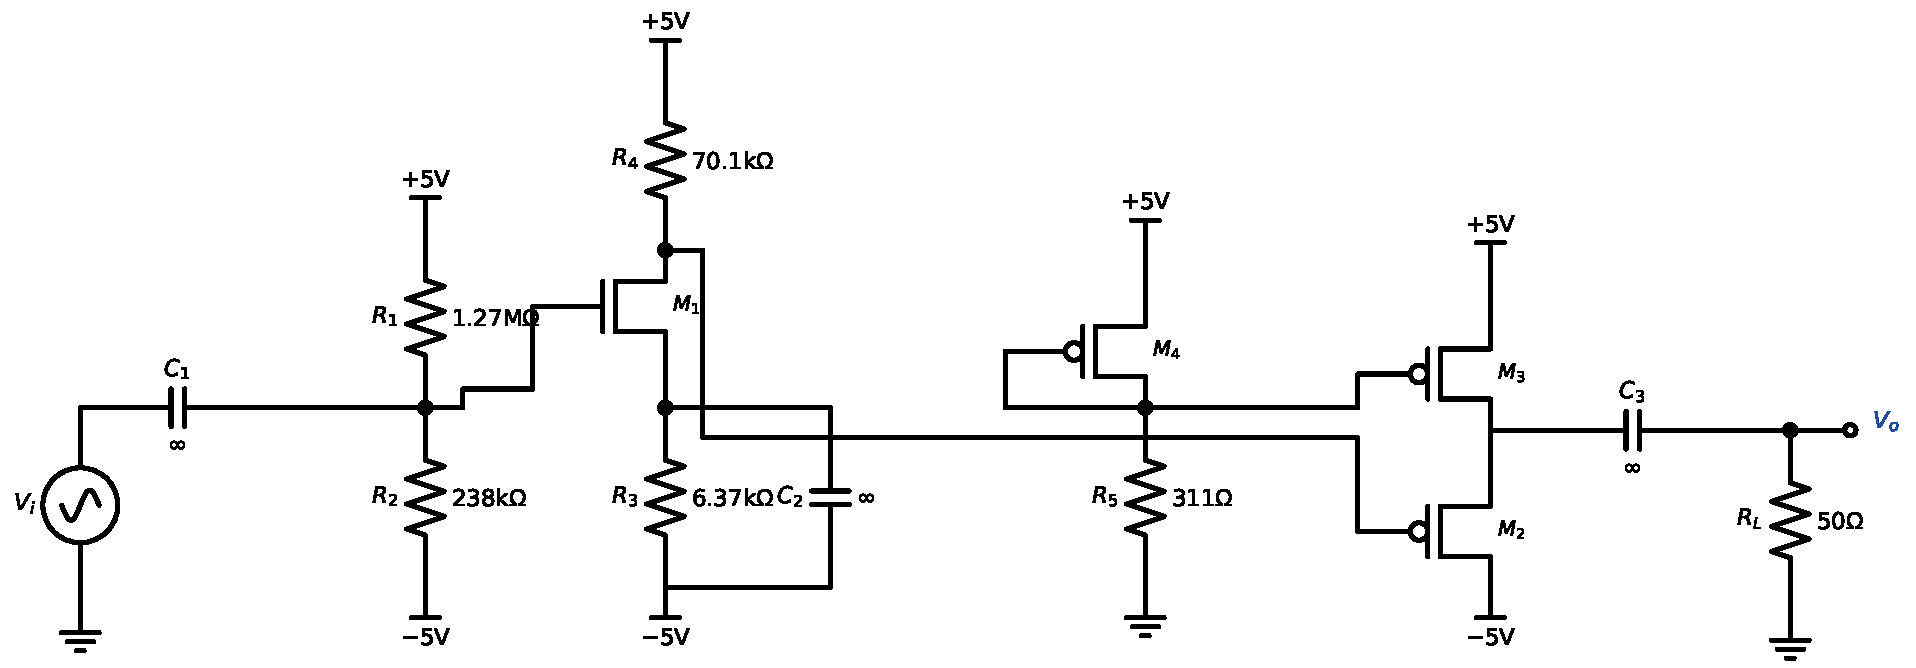
\includegraphics[width=0.85\linewidth,height=6cm,keepaspectratio]{p16_designed}\end{center}

\begin{ansbox}
$R_{1} = 1.27\,\mathrm{M}\Omega$,\quad $R_{2} = 238\,\mathrm{k}\Omega$,\quad $R_{3} = 6.37\,\mathrm{k}\Omega$,\quad $R_{4} = 70.1\,\mathrm{k}\Omega$,\quad $R_{5} = 311\,\Omega$
\end{ansbox}

\newpage
\subsection*{Solution 5E.17 \hfill Hard}
\begin{center}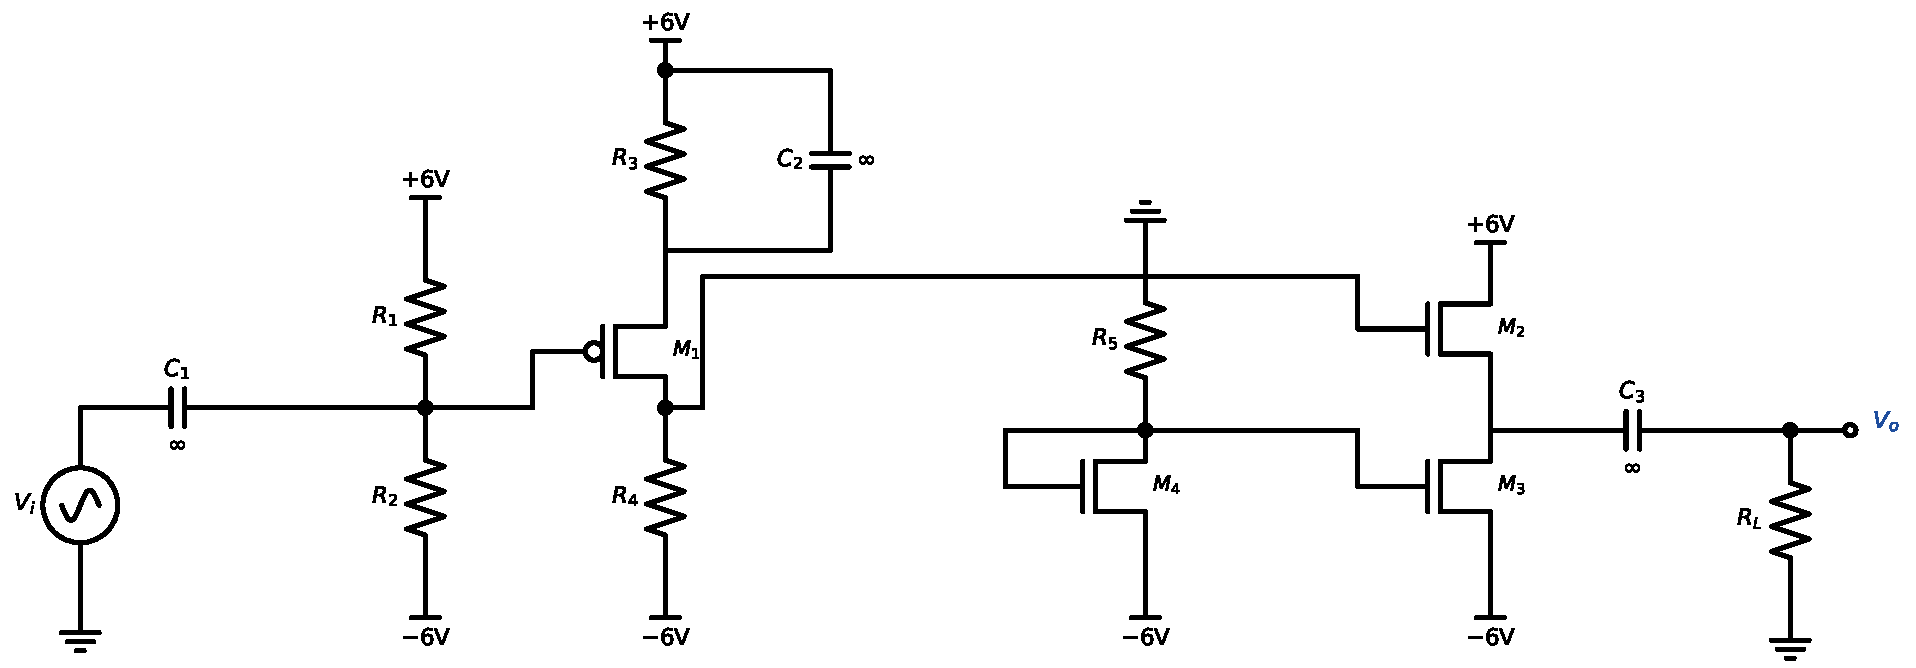
\includegraphics[width=0.9\linewidth,height=6cm,keepaspectratio]{p17_circuit}\end{center}
\solstep{1}{Plan}Follow the procedure of Sample Problem 5: size the output current sink for the load current, then the follower; budget the supply voltage around the drain swing; get $V_{ov1}$ from the gain ($|A_v| = g_mR = 2V_R/V_{ov}$), then the resistors; finally the gate divider from the input resistance. Distortion of a common-source stage: $HD_2 \approx \frac{\hat v_{gs}}{4V_{ov}}$ (from $i_D = \frac{k}{2}(V_{ov} + v_{gs})^2$).
\solstep{2}{Output stage: sink, reference and follower}The sink $M_3$ must deliver the whole peak load current: $I_{D3} \ge \frac{\hat V_o}{R_L} = \frac{2}{75\,\Omega} = 26.7\,\mathrm{m}\mathrm{A}$; use $I_{D3} = 30\,\mathrm{m}\mathrm{A}$ (given). Then $\frac{k_3}{2}V_{ov3}^2 = I_{D3} \Rightarrow V_{ov3} = \sqrt{\frac{2\cdot30\,\mathrm{m}\mathrm{A}}{50\,\mathrm{m}\mathrm{A/V^2}}} = 1.095$\,V.

$M_4$ has the same $V_{GS}$ as $M_3$ but $k_4 = 0.5\,k_3$, so $I_{D4} = 0.5\,I_{D3} = 15\,\mathrm{m}\mathrm{A}$ (same $V_{ov}$).

\[R_5 = \frac{6 - |V_{t}| - V_{ov4}}{I_{D4}} = \frac{6 - 2 - 1.095}{15\,\mathrm{m}\mathrm{A}} = \mathbf{194\,\Omega}\]

The follower $M_2$ carries the same current, $I_{D2} = I_{D3}$, so $V_{ov2} = 1.095$\,V, $g_{m2} = k_2V_{ov2} = 54.8\,\mathrm{m}\mathrm{A/V}$, $1/g_{m2} = 18.3\,\Omega$ and (the sink $M_3$ is a current source, $Z = \infty$) \[A_{v2} = \frac{R_L}{1/g_{m2} + R_L} = \frac{75\,\Omega}{18.3\,\Omega + 75\,\Omega} = 0.8042\]So the drain of $M_1$ must swing $\hat V_d = \hat V_o/A_{v2} = 2.487$\,V and $|A_{v1}| = |A_v|/A_{v2} = 74.61$.
\solstep{3}{Common-source stage}Voltage budget of the $V_{DD} + V_{SS} = 12$\,V branch through $R_3$, $M_1$, $R_4$. At the lowest drain voltage of $M_1$ the follower and the sink must both stay active (the drain of $M_1$ sits one $|V_{GS2}|$ away from the output, which needs $V_{ov3}$ of room above the rail): \[V_{R4} \ge V_{ov3} + V_{ov2} + |V_{t2}| + \hat V_d = 1.1 + 1.1 + 2 + 2.49 = 6.678\,\mathrm{V}\]$M_1$ must stay active at the other extreme: $V_{R3} + V_{ov1} + \hat V_d + V_{R4} \le 12$, and with $V_{ov1} = 2V_{R4}/|A_{v1}|$ (below): \[V_{R4}\left(1 + \frac{2}{|A_{v1}|}\right) \le 12 - V_{R3} - \hat V_d \Rightarrow V_{R4} \le 8.778\,\mathrm{V}\]$V_{R3} = 0.5$\,V (its minimum) and $V_{R4} = 7$\,V (the next multiple of $0.5$\,V above the lower bound).

Gain of the common-source stage ($R_3$ is bypassed, the follower's gate loads nothing): \[|A_{v1}| = g_{m1}R_4 = k_1V_{ov1}\frac{V_{R4}}{\frac{k_1}{2}V_{ov1}^2} = \frac{2V_{R4}}{V_{ov1}} \Rightarrow V_{ov1} = \frac{2\cdot7}{74.61} = 0.1877\,\mathrm{V}\]$I_{D1} = \frac{k_1}{2}V_{ov1}^2 = 17.6\,\mu \mathrm{A}$, $R_4 = \frac{V_{R4}}{I_{D1}} = \mathbf{398\,\mathrm{k}\Omega}$, $R_3 = \frac{V_{R3}}{I_{D1}} = \mathbf{28.4\,\mathrm{k}\Omega}$.

Gate divider: the resistor on the source side of $M_1$ carries $V_{R1} = V_{R3} + |V_{t1}| + V_{ov1} = 1.688$\,V, the other one $V_{R2} = 12 - 1.688 = 10.31$\,V. Both carry the same current ($I_G = 0$): $R_{1} = 1.688X$, $R_{2} = 10.31X$, and the input resistance is their parallel combination: \[R_1\|R_2 = \frac{1.688\cdot10.31}{12}X \ge 100\,\mathrm{k}\Omega \Rightarrow X = 69\,\mathrm{k}\Omega:\quad \mathbf{R_1 = 116\,\mathrm{k}\Omega},\ \mathbf{R_2 = 711\,\mathrm{k}\Omega}\]
\solstep{4}{Check by analysis}DC analysis of the finished circuit (as in sets 5A/5B):\begin{center}\renewcommand{\arraystretch}{1.35}
\begin{tabular}{cccc}
\toprule
 & $I_D$ & $V_{ov}$ & $|V_{DS}|$ \\
\midrule
$M_{1}$ & $17.6\,\mu \mathrm{A}$ & $0.188$\,V & $4.5$\,V \\
$M_{4}$ & $15\,\mathrm{m}\mathrm{A}$ & $1.1$\,V & $3.095$\,V \\
$M_{2}$ & $30\,\mathrm{m}\mathrm{A}$ & $1.1$\,V & $8.095$\,V \\
$M_{3}$ & $30\,\mathrm{m}\mathrm{A}$ & $1.1$\,V & $3.905$\,V \\
\bottomrule
\end{tabular}\end{center}
\begin{itemize}[leftmargin=*,itemsep=2pt]
\item $V_{SD1} = V_{S1} - V_{D1} = 5.5 - 1 = 4.5\,\mathrm{V}$ $\ge V_{ov1} = 0.188$\,V $\Rightarrow$ $M_{1}$ is active \checkmark
\item $M_{4}$ is diode-connected: $V_{DS4} = V_{GS4} > V_{ov4}$, always active \checkmark
\item $V_{DS2} = 6 - V_{S2} = 6 - (-2.095) = 8.1\,\mathrm{V}$ $\ge V_{ov2} = 1.1$\,V $\Rightarrow$ $M_{2}$ is active \checkmark
\item $V_{DS3} = V_{S2} - (-6) = -2.095 - (-6) = 3.9\,\mathrm{V}$ $\ge V_{ov3} = 1.1$\,V $\Rightarrow$ $M_{3}$ is active \checkmark
\item Gain (exact small-signal analysis of the finished circuit): $|A_v| = 60$ \checkmark
\item Input resistance $R_1\|R_2 = 100\,\mathrm{k}\Omega \ge 100\,\mathrm{k}\Omega$ \checkmark
\item Output swing before clipping: $M_1$ leaves saturation at $\hat V_o = 3.47$\,V; $M_3$ leaves saturation at $\hat V_o = 2.81$\,V; $M_2$ leaves saturation at $\hat V_o = 7$\,V; $M_3$ cannot sink more current (current clipping) at $\hat V_o = 2.25$\,V. The smallest is $2.25$\,V $\ge 2$\,V \checkmark
\item THD $\approx HD_2 = \frac{\hat v_{gs1}}{4V_{ov1}} = \frac{2/60}{4\cdot0.188} = 4.4\,\%$ $\le 10\,\%$ \checkmark
\end{itemize}

\begin{center}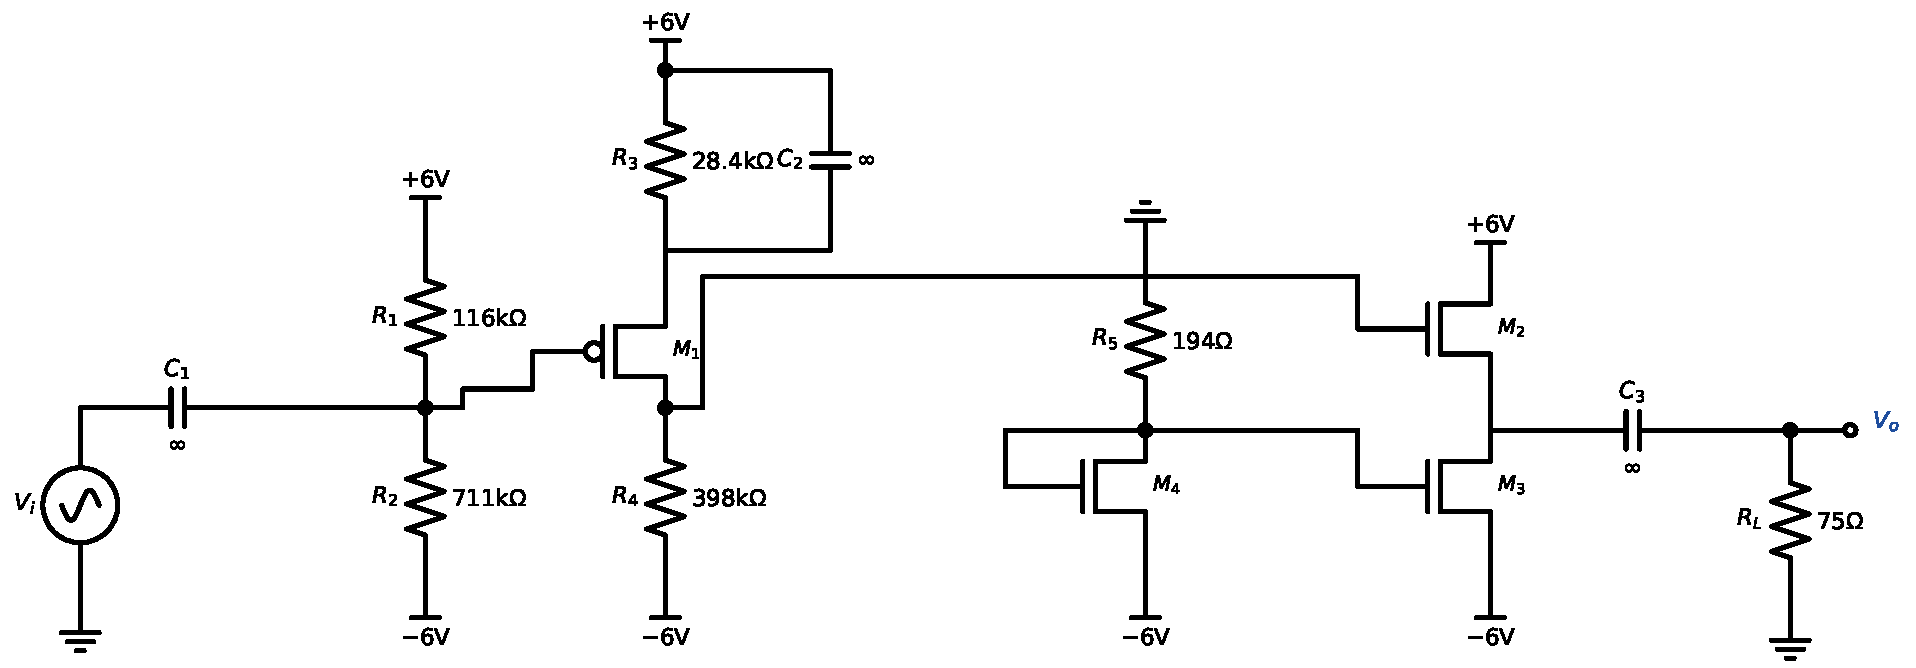
\includegraphics[width=0.85\linewidth,height=6cm,keepaspectratio]{p17_designed}\end{center}

\begin{ansbox}
$R_{1} = 116\,\mathrm{k}\Omega$,\quad $R_{2} = 711\,\mathrm{k}\Omega$,\quad $R_{3} = 28.4\,\mathrm{k}\Omega$,\quad $R_{4} = 398\,\mathrm{k}\Omega$,\quad $R_{5} = 194\,\Omega$
\end{ansbox}

\newpage
\subsection*{Solution 5E.18 \hfill Hard}
\begin{center}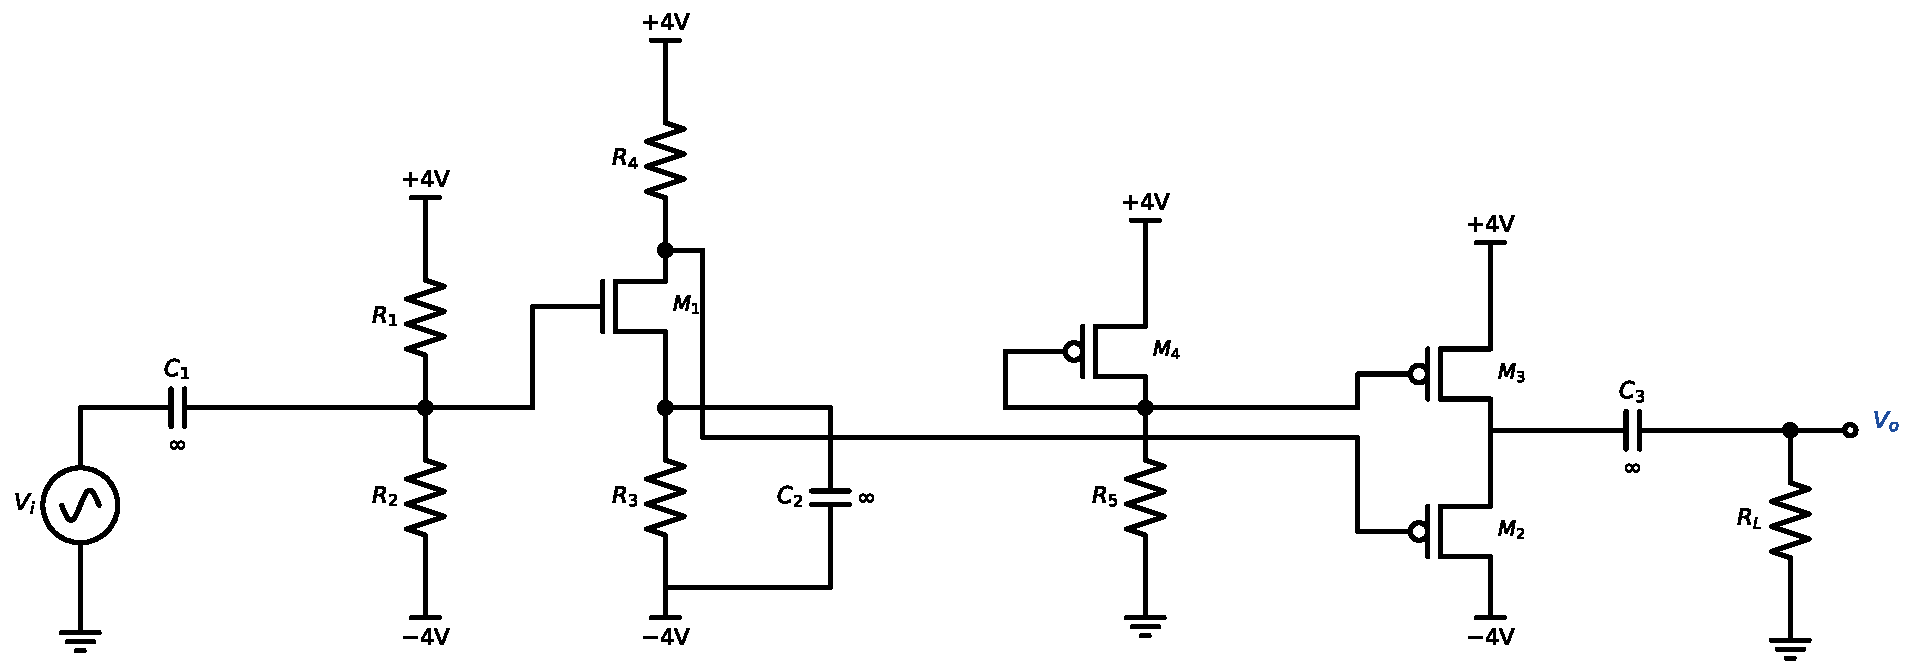
\includegraphics[width=0.9\linewidth,height=6cm,keepaspectratio]{p18_circuit}\end{center}
\solstep{1}{Plan}Follow the procedure of Sample Problem 5: size the output current sink for the load current, then the follower; budget the supply voltage around the drain swing; get $V_{ov1}$ from the gain ($|A_v| = g_mR = 2V_R/V_{ov}$), then the resistors; finally the gate divider from the input resistance. Distortion of a common-source stage: $HD_2 \approx \frac{\hat v_{gs}}{4V_{ov}}$ (from $i_D = \frac{k}{2}(V_{ov} + v_{gs})^2$).
\solstep{2}{Output stage: sink, reference and follower}The sink $M_3$ must deliver the whole peak load current: $I_{D3} \ge \frac{\hat V_o}{R_L} = \frac{1}{100\,\Omega} = 10\,\mathrm{m}\mathrm{A}$; use $I_{D3} = 12\,\mathrm{m}\mathrm{A}$ (given). Then $\frac{k_3}{2}V_{ov3}^2 = I_{D3} \Rightarrow V_{ov3} = \sqrt{\frac{2\cdot12\,\mathrm{m}\mathrm{A}}{50\,\mathrm{m}\mathrm{A/V^2}}} = 0.6928$\,V.

$M_4$ is identical to $M_3$ and has the same $V_{GS}$, so $I_{D4} = I_{D3}$ and $V_{ov4} = V_{ov3}$.

\[R_5 = \frac{4 - |V_{t}| - V_{ov4}}{I_{D4}} = \frac{4 - 1 - 0.6928}{12\,\mathrm{m}\mathrm{A}} = \mathbf{192\,\Omega}\]

The follower $M_2$ carries the same current, $I_{D2} = I_{D3}$, so $V_{ov2} = 0.6928$\,V, $g_{m2} = k_2V_{ov2} = 34.6\,\mathrm{m}\mathrm{A/V}$, $1/g_{m2} = 28.9\,\Omega$ and (the sink $M_3$ is a current source, $Z = \infty$) \[A_{v2} = \frac{R_L}{1/g_{m2} + R_L} = \frac{100\,\Omega}{28.9\,\Omega + 100\,\Omega} = 0.776\]So the drain of $M_1$ must swing $\hat V_d = \hat V_o/A_{v2} = 1.289$\,V and $|A_{v1}| = |A_v|/A_{v2} = 25.77$.
\solstep{3}{Common-source stage}Voltage budget of the $V_{DD} + V_{SS} = 8$\,V branch through $R_3$, $M_1$, $R_4$. At the highest drain voltage of $M_1$ the follower and the sink must both stay active (the drain of $M_1$ sits one $|V_{GS2}|$ away from the output, which needs $V_{ov3}$ of room above the rail): \[V_{R4} \ge V_{ov3} + V_{ov2} + |V_{t2}| + \hat V_d = 0.693 + 0.693 + 1 + 1.29 = 3.674\,\mathrm{V}\]$M_1$ must stay active at the other extreme: $V_{R3} + V_{ov1} + \hat V_d + V_{R4} \le 8$, and with $V_{ov1} = 2V_{R4}/|A_{v1}|$ (below): \[V_{R4}\left(1 + \frac{2}{|A_{v1}|}\right) \le 8 - V_{R3} - \hat V_d \Rightarrow V_{R4} \le 5.764\,\mathrm{V}\]$V_{R3} = 0.5$\,V (its minimum) and $V_{R4} = 4$\,V (the next multiple of $0.5$\,V above the lower bound).

Gain of the common-source stage ($R_3$ is bypassed, the follower's gate loads nothing): \[|A_{v1}| = g_{m1}R_4 = k_1V_{ov1}\frac{V_{R4}}{\frac{k_1}{2}V_{ov1}^2} = \frac{2V_{R4}}{V_{ov1}} \Rightarrow V_{ov1} = \frac{2\cdot4}{25.77} = 0.3104\,\mathrm{V}\]$I_{D1} = \frac{k_1}{2}V_{ov1}^2 = 48.2\,\mu \mathrm{A}$, $R_4 = \frac{V_{R4}}{I_{D1}} = \mathbf{83\,\mathrm{k}\Omega}$, $R_3 = \frac{V_{R3}}{I_{D1}} = \mathbf{10.4\,\mathrm{k}\Omega}$.

Gate divider: the resistor on the source side of $M_1$ carries $V_{R2} = V_{R3} + |V_{t1}| + V_{ov1} = 1.51$\,V, the other one $V_{R1} = 8 - 1.51 = 6.49$\,V. Both carry the same current ($I_G = 0$): $R_{2} = 1.51X$, $R_{1} = 6.49X$, and the input resistance is their parallel combination: \[R_1\|R_2 = \frac{1.51\cdot6.49}{8}X \ge 50\,\mathrm{k}\Omega \Rightarrow X = 40.8\,\mathrm{k}\Omega:\quad \mathbf{R_1 = 265\,\mathrm{k}\Omega},\ \mathbf{R_2 = 61.6\,\mathrm{k}\Omega}\]
\solstep{4}{Check by analysis}DC analysis of the finished circuit (as in sets 5A/5B):\begin{center}\renewcommand{\arraystretch}{1.35}
\begin{tabular}{cccc}
\toprule
 & $I_D$ & $V_{ov}$ & $|V_{DS}|$ \\
\midrule
$M_{1}$ & $48.2\,\mu \mathrm{A}$ & $0.31$\,V & $3.5$\,V \\
$M_{4}$ & $12\,\mathrm{m}\mathrm{A}$ & $0.693$\,V & $1.693$\,V \\
$M_{3}$ & $12\,\mathrm{m}\mathrm{A}$ & $0.693$\,V & $2.307$\,V \\
$M_{2}$ & $12\,\mathrm{m}\mathrm{A}$ & $0.693$\,V & $5.693$\,V \\
\bottomrule
\end{tabular}\end{center}
\begin{itemize}[leftmargin=*,itemsep=2pt]
\item $V_{DS1} = V_{D1} - V_{S1} = 4.501\times 10^{-15} - (-3.5) = 3.5\,\mathrm{V}$ $\ge V_{ov1} = 0.31$\,V $\Rightarrow$ $M_{1}$ is active \checkmark
\item $M_{4}$ is diode-connected: $V_{SD4} = V_{SG4} > V_{ov4}$, always active \checkmark
\item $V_{SD3} = 4 - V_{D3} = 4 - 1.693 = 2.31\,\mathrm{V}$ $\ge V_{ov3} = 0.693$\,V $\Rightarrow$ $M_{3}$ is active \checkmark
\item $V_{SD2} = V_{D3} - (-4) = 1.693 - (-4) = 5.69\,\mathrm{V}$ $\ge V_{ov2} = 0.693$\,V $\Rightarrow$ $M_{2}$ is active \checkmark
\item Gain (exact small-signal analysis of the finished circuit): $|A_v| = 20$ \checkmark
\item Input resistance $R_1\|R_2 = 50\,\mathrm{k}\Omega \ge 50\,\mathrm{k}\Omega$ \checkmark
\item Output swing before clipping: $M_1$ leaves saturation at $\hat V_o = 2.48$\,V; $M_3$ leaves saturation at $\hat V_o = 1.61$\,V; $M_2$ leaves saturation at $\hat V_o = 5$\,V; $M_3$ cannot sink more current (current clipping) at $\hat V_o = 1.2$\,V. The smallest is $1.2$\,V $\ge 1$\,V \checkmark
\item THD $\approx HD_2 = \frac{\hat v_{gs1}}{4V_{ov1}} = \frac{1/20}{4\cdot0.31} = 4\,\%$ $\le 10\,\%$ \checkmark
\end{itemize}

\begin{center}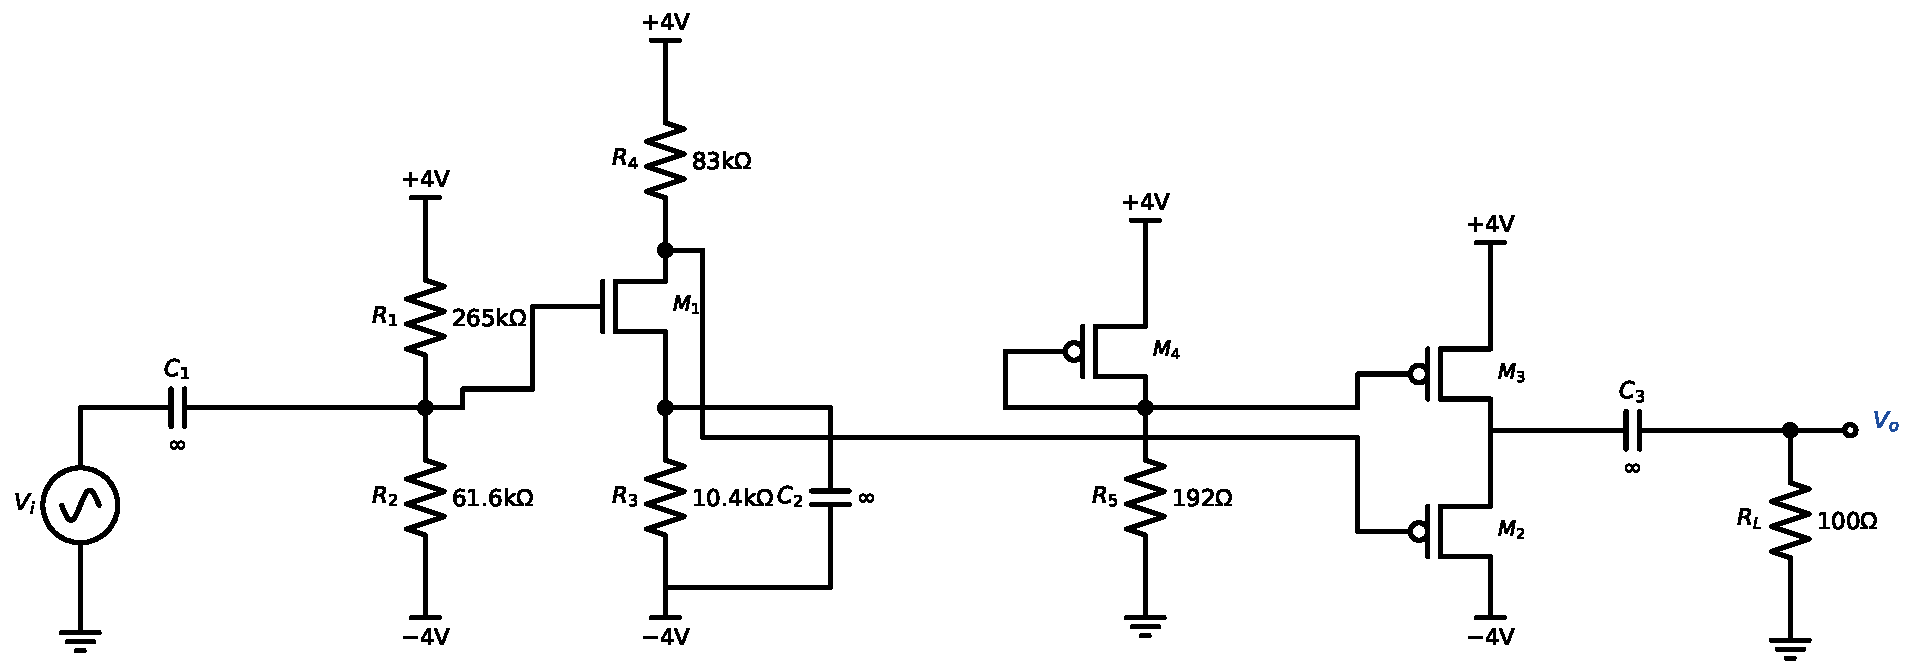
\includegraphics[width=0.85\linewidth,height=6cm,keepaspectratio]{p18_designed}\end{center}

\begin{ansbox}
$R_{1} = 265\,\mathrm{k}\Omega$,\quad $R_{2} = 61.6\,\mathrm{k}\Omega$,\quad $R_{3} = 10.4\,\mathrm{k}\Omega$,\quad $R_{4} = 83\,\mathrm{k}\Omega$,\quad $R_{5} = 192\,\Omega$
\end{ansbox}

\end{document}
